
% -------------------------------------------------------------------------------------------------
%      MDSG Latex Framework
%      ============================================================================================
%      File:                  main.tex
%      Author(s):             Michael Duerr
%      Version:               1
%      Creation Date:         30. Mai 2010
%      Creation Date:         30. Mai 2010
%
%      Notes:                 - This represents the document root of this template
%                             - Binding correction is 12mm. In case you change this value, you
%                               may also need to adapt the value of \bcorlength in mdsg.sty
%                             - Switch `babel' package options `english' and `ngerman' in case
%                               your thesis is in English
%                             - if you prefer to use utf8 encoding, uncomment the corresponding
%                               line `\usepackage[utf8]{inputenc}' and comment the line
%                               `\usepackage[latin1]{inputenc}'. To compile this example you also
%                               need to include the corresponding introduction example file i.e.
%                               `introduction-UTF8.tex' or `introduction-ISO8859-1.tex'
% -------------------------------------------------------------------------------------------------
%
\documentclass[bibliography=totoc,listof=totoc,index=totoc,twoside=true,BCOR=12mm,DIV=12]{scrbook}
%\KOMAoptions{draft=true}                         % uncomment if you want to visualise overful hbox
%\KOMAoptions{chapterprefix=true}                 % uncomment if you like "Chapter" in front of
                                                  % chapter number
%\KOMAoptions{appendixprefix=true}                % uncomment if you like "Appendix" in front of
                                                  % appendix number
%\KOMAoptions{...}                                % feel free to add additional KOMA options
%
% =================================================================================================
% set encoding
% -------------------------------------------------------------------------------------------------
%
\usepackage[utf8]{inputenc}                       % uncomment if you prefer utf8 encoding
%\usepackage[latin1]{inputenc}                    % uncomment if you prefer latin1 encoding
%
% =================================================================================================
% load mdsg style
% -------------------------------------------------------------------------------------------------
%
%\usepackage[diplom]{mdsg}                        % uncomment the corresponding option
%\usepackage[fopra]{mdsg}
%\usepackage[bachelor]{mdsg}
\usepackage[master]{mdsg}
%
% =================================================================================================
% initialize macros
% -------------------------------------------------------------------------------------------------
%
\lmutitle{Organisation von Bloom-Filtern \\zur effizienten k-nächste-Nachbarn-Suche \\in kontextzentrischen sozialen Netzen}                       % title: you can force a new line by
%\lmutitle{Titel \\ der \\ Arbeit}                % inserting `\\'. However, this will cause
                                                  % a hyperref warning!
\lmustudentone{Judith Greif}                    	 % first author's name
%\lmustudenttwo{Max2 Mustermann2}                 % second author's name
%\lmustudentthree{Max3 Mustermann3}               % third author's name
%\lmustudentfour{Max4 Mustermann4}                % fourth author's name

\lmuprofone{Prof. Dr. Claudia Linnhoff-Popien}    % first supervisor's name
%\lmuproftwo{Prof. Dr. Max Mustermann}             % second supervisor's name
                                                  % (uncomment if not needed)
%\lmuprofthree{Prof. Dr. Max2 Mustermann2}         % third supervisor's name
                                                  % (uncomment if not needed)
\lmuadvisorone{Mirco Schönfeld}                    % first advisor's name
\lmuadvisortwo{Dr. Martin Werner}                    % second advisor's name
                                                  % (uncomment if not needed)
%\lmuadvisorthree{Betreuer Name3}                  % third advisor's name
                                                  % (uncomment if not needed)
%\lmudraftdate{\today}                             % only for versioning during work!
                                                  % (uncomment for final version!)
\lmudeadline{26. Juli 2016}                      % deadline (day of submission)
%
% =================================================================================================
% package selection (add additional packages if needed)
% -------------------------------------------------------------------------------------------------
%
%\usepackage{layout}                              % see documentation of this package
\usepackage{cmap}                                 % to produce searchable PDF
\usepackage[T1]{fontenc}                          % split german words with umlaut
\usepackage{lmodern}
% \usepackage[ngerman, english]{babel}              % for german toc, ...
\usepackage[english,ngerman]{babel}
\usepackage{bibgerm}                              % for german bibliography index
\usepackage{tabularx}                             % more flexible table environment
\usepackage{booktabs}                             % high quality tables
\usepackage{rotating}                             % for generation of landscape tables
\usepackage{multirow}                             % for multirow cells inside tables
\usepackage{amssymb,amsmath}                      % powerful math package
\usepackage{hyperref}                             % for hyperlinks
\lmuhypersetup                                    % write some pdf properties
\usepackage{flafter}                              % force floats to appear after their reference
\usepackage{subfig}                               % to allow for side by side graphics (subfloats)
\usepackage{pdflscape}                            % enable rotation of landscape pages
\usepackage{hyphenat}                             % proper hyphenation for bla_bla to bla_-bla
\usepackage[all]{hypcap}                          % correct captions
\usepackage{url}                                  % nicer url style
\usepackage{enumitem}                             % for tight lists
\usepackage{textcomp}

\setcounter{tocdepth}{3}                          % sectioning depth in toc
\setcounter{secnumdepth}{3}                       % sectioning depth in text

\graphicspath{{./pictures/}}                      % put all graphics here
% -------------------------------------------------------------------------------------------------
%      MDSG Latex Framework
%      ============================================================================================
%      File:                  hyphenation.tex
%      Author(s):             Michael Duerr
%      Version:               1
%      Creation Date:         30. Mai 2010
%      Creation Date:         30. Mai 2010
%
%      Notes:                 - Instruction \hypenation cannot handle special characters like umlaute
%                               as well as  "a and \"a. Split such words in your text.
%
% -------------------------------------------------------------------------------------------------
%
\hyphenation{Ba-che-lor-ar-}
%\hyphenation{...}                           % further hyphenation examples
                               % this file holds words latex cannot split
%
% =================================================================================================
% start of document
% -------------------------------------------------------------------------------------------------
%
\begin{document}
    \setlist{noitemsep}                           % for tight lists
    \lmufront                                     % title pages
    \newpage
    \cleardoublepage
    \lmuaffirmation                               % affirmation (work is my own work)
    \newpage
    \cleardoubleemptypage
    \thispagestyle{empty}
    % -------------------------------------------------------------------------------------------------
%      MDSG Latex Framework
%      ============================================================================================
%      File:                  abstract.tex
%      Author(s):             Michael Duerr
%      Version:               1
%      Creation Date:         30. Mai 2010
%      Creation Date:         30. Mai 2010
%
%      Notes:                 - Place your abstract here
% -------------------------------------------------------------------------------------------------
%
\vspace*{2cm}

\begin{center}
    \textbf{Abstract}
\end{center}

\vspace*{1cm}

\noindent Ubiquitous computing und die Zunahme mobiler Endgeräte haben zu neuen Kommunikationsmustern im Internet geführt: Weg von adressbasiertem Routing und Ende-zu-Ende-Kommunikation hin zu \textit{Information-centric Networking}. Kontextzentrische soziale Netze sind ein Ansatz, dem Rechnung zu tragen. Kommunikation basiert darin nicht auf Online-Freundschaft, sondern allein auf Kontext-Ähnlichkeit. Das kontextzentrische soziale Netz AMBIENCE verwendet Bloom-Filter, um Nachrichten zu kodieren, speichern und anzufragen. Diese müssen so an einem Host organisiert werden, dass die \textit{k} nächsten Nachbarn zu einem Anfragefilter möglichst schnell und effizient gefunden werden. Die vorliegende Arbeit optimiert das mengentheoretische Problem der \textit{k}-nächsten-Nachbarn-Suche für dieses Szenario. Dazu wurde eine Indexstruktur für Bloom-Filter basierend auf einem B$^+$-Baum entwickelt. Die Bloom-Filter werden darin nach ihren Teil- und Obermengenbeziehungen organisiert, der \textit{BloomFilterTree}. Bei der \textit{k}-nächsten-Nachbarn-Suche wird nur der beste Pfad im Baum verfolgt und Teilbäume möglichst früh abgeschnitten. Kriterien für die Evaluation waren Ergebnisqualität, CPU-Zeit, Zeitkomplexität, Speicherbedarf und Aufbaukosten. Im verwendeten Versuchsaufbau ließen sich Zeitkomplexität und CPU-Zeit der \textit{k}-nächste-Nachbarn-Suche mit dem BloomFilterTree um bis zu 68\% bzw. 87\% reduzieren.                        % abstract
    \thispagestyle{empty}
    \frontmatter                                  % start roman numbering
    \tableofcontents                              % toc
    \mainmatter                                   % start alpha numbering
    
    %\DefineVerbatimEnvironment{Sinput}{Verbatim}{xleftmargin=2em}
    %\DefineVerbatimEnvironment{Soutput}{Verbatim}{xleftmargin=2em}
    %\DefineVerbatimEnvironment{Scode}{Verbatim}{xleftmargin=2em}
    %\fvset{listofparameters}={\setlength{\topsep}{Opt}}}
    %\renewenvironment{Schunk}{\vspace{\topsep}}{\vspace{\topsep}}
%
% =================================================================================================
% place your document text here (take care of encoding)
% -------------------------------------------------------------------------------------------------
%
    \chapter{Einleitung}\label{ch:einleitung}
%Einleitung
%Motivieren Sie ihre Arbeit. Warum ist diese Arbeit relevant, was erwartet die LeserInnen.
Referenzen bis jetzt: \cite{Agarwal2006}, \cite{Ahlgren2012}, \cite{Bayardo2007}, \cite{Broder2004}, \cite{Byers2002}, \cite{Duerr2010}, \cite{Hellerstein1994}, \cite{Lehman1986}, \cite{Nafe2005}, \cite{Qiao2014}, \cite{Ruppel2014}, \cite{Sarwat2012}, \cite{Schnell2013}, \cite{Schoenfeld2014}, \cite{Shiraki2009}, \cite{Werner2015}, \cite{Yang2002}, \cite{Zhang2012}, \cite{Zhu2004}, \cite{Jannink1995}.
\section{Problembeschreibung}\label{sec:problem}

%\subsection{Referenz auf anderen Text}
%Es ist auch möglich auf andere Stellen im Text z.B. Kapitel \ref{subsec:sources} zu verweisen.
%\subsection{Tabellen}
%Es gibt schöne Möglichkeiten Tabellen einzubinden wie z.B. Tabelle \ref{tab:CommonParameterSettings}.
%\begin{center}
%\begin{table}[htbp]
%{\small
%\begin{center}
%\begin{tabular}[center]{lrlc}
%\toprule
%Parameter & Value & (Unit) & Available for Chord \\
%\midrule
%Query timeout & 10 & seconds & $\surd$ \\
%Republish timeout & 300 & seconds & $\surd$ \\ % explain this value...
%Stabilize timeout & 5 & seconds & $\surd$ \\
%Fix fingers timeout & 30 & seconds & $\surd$ \\
%Message timeout & 1 & second & $\surd$ \\
%Connect timeout & 10 & seconds & $\surd$ \\
%Ping superpeer timeout & 5 & seconds & $\times$ \\
%Cost-Optimality estimation timeout & 20 & seconds & $\times$ \\
%Significance for change in number of superpeers & 10 & percent & $\times$ \\
%Significance for change in estimations  & 10 & percent & $\times$ \\
%Number of permanent superpeers & 32 & nodes & $\times$ \\
%Mean number of peers & 1000 & nodes & $\surd$ \\
%Mean number of lookups per hour & 60 & queries & $\surd$ \\
%Mean number of shared InfoProfiles per node & 20 & & $\surd$ \\
%Identifier space & 16 & bits & $\surd$ \\
%Direct insertion acknowledgment & true & bool & $\times$ \\
%Direct query responses & true & bool & $\times$ \\
%Force query resolution & true & bool & $\surd$  \\
%\bottomrule
%\end{tabular}
%\end{center}
%} % end of tiny
%\caption[Simulation parameter settings]{Common simulation parameter settings.\label{tab:CommonParameterSettings}}
%\end{table}
%\end{center}
%
%\subsection{Bilder}
%Man kann sehr einfach Bilder einbinden so wie z.B. in Abbildung \ref{fig:pic0}.
%\begin{figure}[hpbt]
%  \centering
%  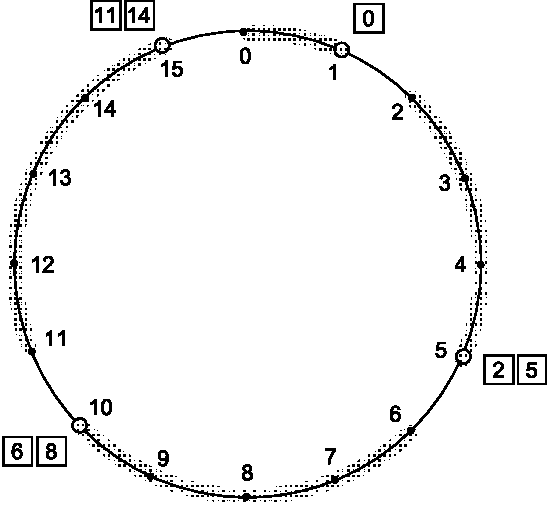
\includegraphics[width=0.4\textwidth]{pictures/pic0}\\
%  \caption[Example of a $4$-bit Chord identifier circle]{Example of a $4$-bit Chord identifier circle.
%  The responsibility ranges for each peer are accentuated in light gray}\label{fig:pic0}
%\end{figure}
%Es lassen sich auch mehrere Bilder nebeneinander platzieren wie z.B. in Abbildung
%\ref{fig:multipic} zu sehen ist.
%\begin{figure}[hpbt]
% \centering
%  %%----start of first subfigure----
%  \subfloat[FIFO size limited to 20 entries]{
%   \label{fig:multipic:a} %% label for first subfigure
%   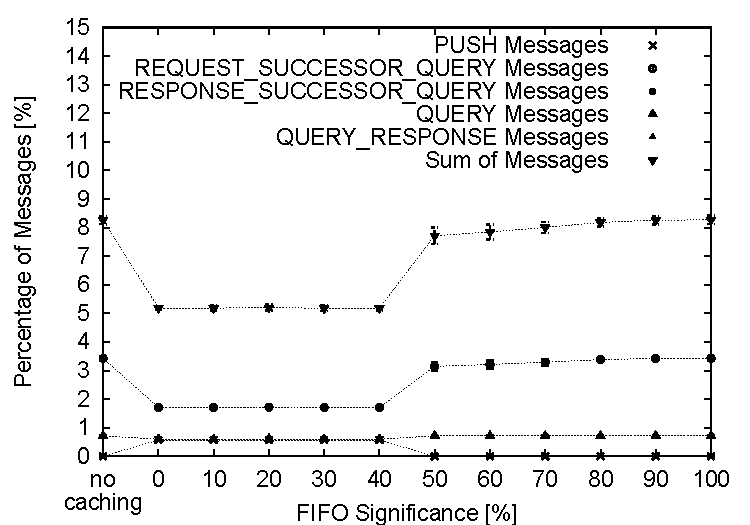
\includegraphics[width=0.48\linewidth]{pic1}}
%  \hspace{0.01\textwidth}
%  %%----start of second subfigure----
%  \subfloat[FIFO size limited to 30 entries]{
%   \label{fig:multipic:b} %% label for second subfigure
%   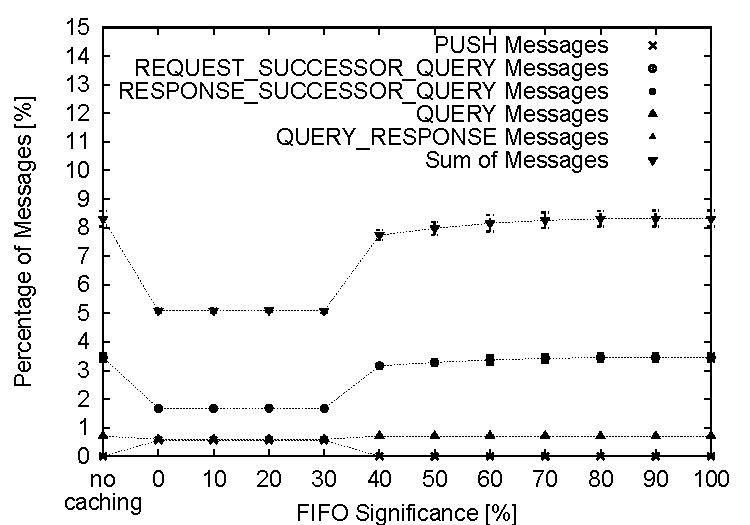
\includegraphics[width=0.48\linewidth]{pic2}}\\[0pt] % horizontal break
%  %%----start of third subfigure----
%  \subfloat[FIFO size limited to 40 entries]{
%   \label{fig:multipic:c} %% label for third subfigure
%   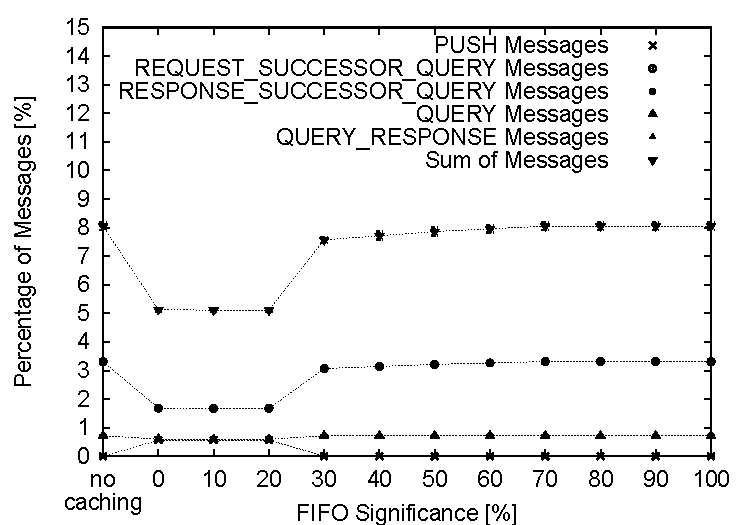
\includegraphics[width=0.48\linewidth]{pic3}}
%  \hspace{0.01\textwidth}
%  %%----start of fourth subfigure----
%  \subfloat[FIFO size limited to 50 entries]{
%   \label{fig:multipic:d} %% label for fourth subfigure
%   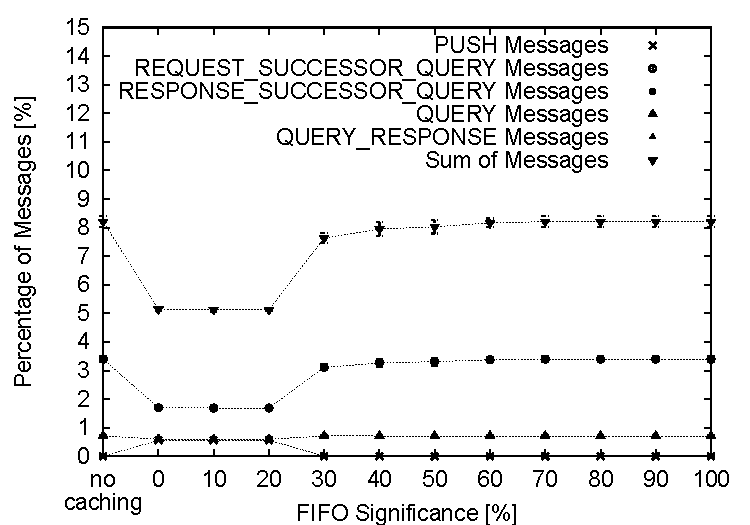
\includegraphics[width=0.48\linewidth]{pic4}}
% \caption[Observed message fractions and 95\% confidence intervals for Chord]{Observed message fractions and 95\% confidence intervals for Chord without the influence of churn. The FIFO capacity varies from 20 (\ref{fig:multipic:a}) -- 50 (\ref{fig:multipic:d}) entries (decadic steps).}
% \label{fig:multipic} %% label for entire figure
%\end{figure}
%
%\subsection{Programm Code}
%Eine elegante Möglichkeit, Programmtext einzubinden, lässt sich mit dem listings-Paket erreichen.
%Das \verb|HelloWorld| Programm aus Listing \ref{lst:hw} hat in Zeile \ref{line:hw3} übrigens einen Programmierfehler.
%\begin{lstlisting}[float=htp,caption=Hello World,label=lst:hw,language=Java, numbers=left, numberstyle=\tiny, stepnumber=2, numbersep=8pt, escapeinside={//@}{@//},backgroundcolor=\color{yellow},xleftmargin=3ex,xrightmargin=1ex]
%public class HelloWorld {
%    public static void main(String[] args) {
%        Syste.out.println("Hello, World"); //@\label{line:hw3}@//
%    }
%}
%\end{lstlisting}
    \chapter{Hintergrund}\label{ch:hintergrund}
Im Folgenden wird das Konzept des \textit{kontextzentrischen sozialen Netzes} erläutert, das dieser Arbeit zu Grunde liegt. Anschließend werden mengentheoretische und probabilistische Grundlagen und Verfahren sowie Daten- und Indexstrukturen dargestellt, die Eingang in diese Arbeit gefunden haben. Es wird erläutert, inwiefern sie für das soziale Online-Netz AMBIENCE relevant sind oder darin verwendet werden. 
\section{Kontextzentrische soziale Netze}\label{sec:kontext}
Mit Zunahme der mobilen Endgeräte und dem Erfolgszug des Smartphones lässt sich eine Tendenz beobachten, die von bestehenden sozialen Online-Netzwerken wenig abgebildet wird: Weg von adressbasiertem Routing und Ende-zu-Ende-Kommunikation hin zu \textit{context-awareness} und \textit{information-centric networking}. 

Der Begriff context-awareness wurde von Schilit et al. 1994 geprägt und bezeichnet die Nutzung von Kontextinformationen als Informationsquelle für Anwendungen und Netzwerke \cite{Schilit1994}. Information-centric networking (ICN) bezeichnet ein neuartiges Konzept für Netzwerke, die nicht auf Ende-zu-Ende- oder Sender/Empfänger-Kommunikation basieren, sondern auf den im Netzwerk vorhandenen Informationen \cite{Ahlgren2012}. 
Der Begriff \textit{Kontext} im Zusammenhang mit interaktiven Anwendungen wurde bereits in den 90er Jahren geprägt. Die klassische Definition von Dey und Abowd lautet: 
\begin{quote}
\textit{"`Context is any information that can be used to characterize the situation of an entity. An entity is a person, place, or object that is considered relevant to the interaction between a user and an application including the user and application themselves."'} \cite{Dey1999} 
\end{quote}
Diese Definition lässt sich für soziale Online-Netze eingrenzen auf 
\begin{quote}
\textit{"`[...] any information that can be used to infer aspects of the surroundings of an entity in a way, in which some applications may have interest. Surroundings include all information that could possibly impact the behaviour of the entity."'} \cite{Werner2015}
\end{quote}
Ein kontextzentrisches soziales Netz ist also ein soziales Online-Netz, das auf Kontext-Variablen wie Ort und Zeit als Informationsquellen basiert und in der Regel dezentral organisiert ist, z.B. durch eine Peer-to-Peer- statt einer Client/Server-Architektur. Kommunikation beruht darin allein auf Kontext-Ähnlichkeit, nicht auf Online-Freundschaft: 
\begin{quote}
\textit{"`A context-centric online social network is an online social network in which the edges of the social graph are defined from context information and context matching algorithms. An edge between two profiles exists for a fixed information object if and only if the two profiles share the relevant context as defined by the publisher."'} \cite{Werner2015}
\end{quote}
\paragraph*{AMBIENCE}
AMBIENCE ist ein soziales Online-Netzwerk, das 2015 als Prototyp implementiert wurde und sich an diesem neuen Paradigma orientiert. Die vorliegende Arbeit hat das Ziel, einen spezifischen Aspekt des Netzwerks zu optimieren, nämlich die Organisation der Nachrichten für \textit{k}-nächste-Nachbarn-Anfragen an einen Host. Nachrichten und Anfragen werden in AMBIENCE als Bloom-Filter kodiert. Bei einer Anfrage wird also ein Anfrage-Filter mit einer Menge von Bloom-Filtern verglichen, die an einem Host gespeichert sind. Aktuell werden die Filter dort einfach als unsortierte Liste gespeichert. Die Laufzeit für \textit{k}-nächste-Nachbarn-Anfragen an einen Host mit \textit{n} Filtern liegt damit in $O(n^2)$. Dieses Laufzeitverhalten gilt es zu optimieren, wenn das Netzwerk wachsen und über den Status eines Prototypen hinaus erfolgreich sein soll. 
\section{Bloom-Filter}\label{sec:bloom}
Ein Bloom-Filter ist eine probabilistische Datenstruktur zur Beschreibung von Mengen und wurde in der ursprünglichen Form 1970 von Burton H. Bloom eingeführt \cite{Bloom1970}. Er besteht aus einem Bit-Array der festen Länge \textit{m}, dessen Elemente zunächst alle auf 0 gesetzt sind. Das Einfügen von Informationsobjekten basiert auf der Berechnung einer festen Anzahl unabhängiger Hashfunktionen \textit{k}, die positive Werte kleiner als \textit{m} annehmen. Soll ein Objekt in den Filter eingefügt werden, werden seine Hashwerte berechnet und die entsprechenden Bits im Filter gesetzt \cite{Broder2004}. 

Die Hashwerte werden für Anfragen an den Filter verwendet. Ist ein Objekt im Filter enthalten, sind seine charakteristischen Bits gesetzt worden, d.h. man kann eine Anfrage nach seinen Hashwerten durchführen und mit großer Wahrscheinlichkeit ermitteln, ob es im Filter vorhanden ist. Sind ein oder mehrere Bits des Anfrageobjekts nicht gesetzt, ist es mit Sicherheit nicht im Filter vorhanden. Es gibt also keine falsch negativen Antworten. Allerdings kann es sein, dass ein Element nicht in den Filter eingefügt wurde, obwohl alle seine Bits gesetzt sind (falsch positive Antworten). Grund dafür ist die Kollisionseigenschaft von Hashfunktionen, die ein großes Universum von Objekten auf einen sehr viel kleineren Wertebereich, hier die Länge des Bloom-Filters, abbilden. Es kann somit zu Kollisionen zwischen unterschiedlichen Informationsobjekten bzw. ihren charakteristischen Hashwerten kommen. 

Die Falsch-Positiv-Rate eines Bloom-Filters ist abhängig von \textit{m}, \textit{k} und der Anzahl der eingefügten Elemente \textit{n}. Dieser Zusammenhang ist von zentraler Bedeutung, um die Vorteile von Bloom-Filtern richtig nutzen zu können. Die Falsch-Positiv-Rate lässt sich wie folgt bestimmen \cite{Broder2004}: 

Nach dem Einfügen aller Objekte in den Filter beträgt die Wahrscheinlichkeit dafür, dass ein beliebiges Bit den Wert 0 hat, 
\[\left(1 - \frac{1}{m}\right)^{kn}\approx e^{-kn/m}.\]
Unter der Voraussetzung optimaler, zufälliger Hashfunktionen darf man $p = e^{-kn/m}$ annehmen und erhält für die Falsch-Positiv-Rate
\[f = \left(1 - \left(1-\frac{1}{m}\right)^{kn}\right)^k\approx\left(1 - e^{-kn/m}\right)^k = (1-p)^k.\]

Das bedeutet: Die Falsch-Positiv-Rate eines Bloom-Filters steigt mit der Anzahl der eingefügten Objekte und der Anzahl der verwendeten Hashfunktionen, die zum Einfügen jedes Objekts verwendet werden, und sinkt mit steigender Größe des Daten-Arrays im Bloom-Filter. Offensichtlich sind also drei Performanz-Metriken im Bloom-Filter von Bedeutung, die mit Hilfe der Parameter \textit{m}, \textit{k} und \textit{f} beeinflusst werden können: Filtergröße, Geschwindigkeit und Falsch-Positiv-Rate.  

Abhängig vom Anwendungsfall kann der Anwender also entscheiden, welche Metrik(en) für den Bloom-Filter optimiert werden sollen. Werden Bloom-Filter zur Übermittlung von Nachrichten in einem Verteilten System genutzt, wird man womöglich eine höhere Falsch-Positiv-Rate zu Gunsten einer kleineren Nachrichtenlänge bzw. Filtergröße in Kauf nehmen \cite{Mitzenmacher2002}. In einem Datenbank-Managementsystem wird man hingegen versuchen, die Falsch-Positiv-Rate möglichst niedrig zu halten, da jeder Zugriff auf den Sekundärspeicher rechen- und zeitaufwändig ist. Es liegt also nahe, falsch positive Ergebnisse und damit überflüssige Plattenzugriffe möglichst zu vermeiden. Wieder andere Anwendungen müssen möglichst schnell Ergebnisse liefern wie z.B. der Abgleich mit einer schwarzen Liste von Webseiten. Wird eine Webseite auf Grund eines falsch positiven Ergebnisses versehentlich als bösartig eingestuft, obwohl sie keinen schädlichen Inhalt hat, ist dies sicherlich eher zu tolerieren als ein unverhältnismäßig hoher Zeitaufwand für den Abgleich. In diesem Fall würde man vermutlich eher die Filtergröße reduzieren, um rasch ein Suchergebnis zu erhalten, und eine erhöhte Falsch-Positiv-Rate in Kauf nehmen. 

Aus der Kollisionseigenschaft folgt auch, dass ein einmal eingefügtes Objekt nicht mehr aus einem Bloom-Filter entfernt werden kann. Das könnte offensichtlich zu falsch negativen Ergebnissen für andere Objekte führen. Abbildung \ref{fig:pic0} zeigt ein Beispiel für einen Bloom-Filter, in den die Objekte \textit{x}, \textit{y} und \textit{z} eingefügt wurden. Das Objekt \textit{w} ist nicht im Filter vorhanden\footnote{Bildnachweis: \url{https://commons.wikimedia.org/wiki/File:Bloom_filter.svg} (17.07.2016).}.
\begin{figure}[hpbt]
  \centering
  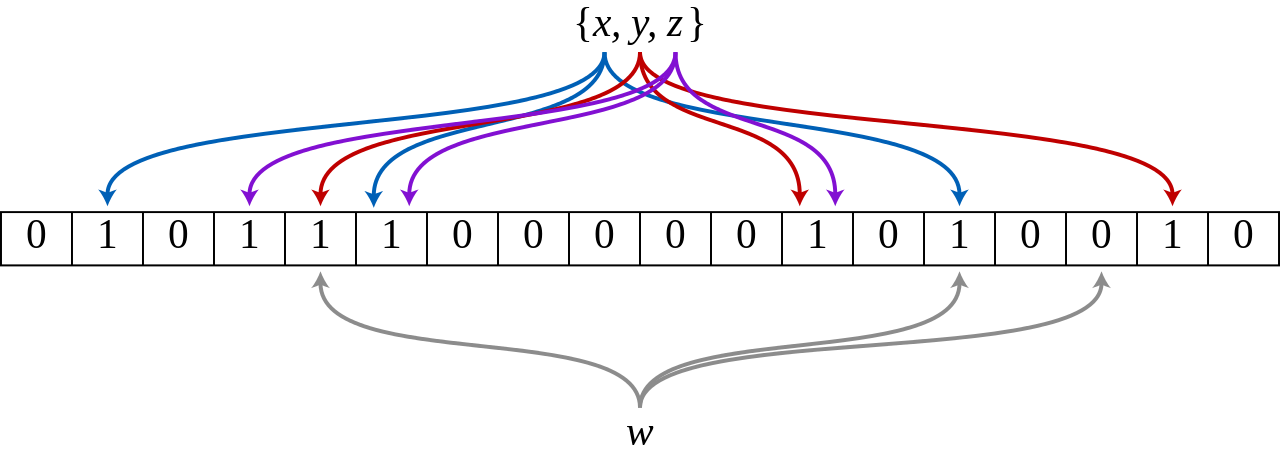
\includegraphics[width=0.8\textwidth]{pictures/1280px-Bloom_filter.png}\\
  \caption[Bloom-Filter]{Bloom-Filter.}\label{fig:pic0}
\end{figure}
\subsection{Distanzmaße}\label{sec:distanzmasse}
Um die Ähnlichkeit zweier Mengen zu ermitteln, werden unterschiedliche Distanzmetriken oder Ähnlichkeitsmaße verwendet. Für den Vergleich von Bloom-Filtern und insbesondere für die \textit{k}-nächste-Nachbarn-Suche muss ein geeignetes Ähnlichkeitsmaß zur Anwendung kommen. Bayardo et al. verwenden dazu die \textit{Kosinus-Ähnlichkeit} \cite{Bayardo2007}, Sakuma und Sato definieren die Ähnlichkeit von Bloom-Filtern als die Anzahl gleicher 1-Bits \cite{Sakuma2011}. Ist diese für zwei Filter identisch, werden die Bit-Arrays negiert und die Anzahl gleicher 0-Bits ermittelt. 

In AMBIENCE wird eine Abschätzung der \textit{Jaccard-Distanz} zur Ermittlung der Ähnlichkeit von Bloom-Filtern verwendet. Die Jaccard-Distanz zwischen zwei Mengen \textit{A} und \textit{B} ist definiert als 
\[J_{\delta}(A,B) = 1 - J(A,B) = \frac{|A\cap B| - |A\cup B|}{|A\cup B|}, \]
wobei 
\[J(A,B) = \frac{|A\cap B|}{|A\cup B|}\] den \textit{Jaccard-Koeffizienten} bezeichnet. Die Jaccard-Distanz nimmt Werte im Bereich $\left[0,1\right]$ an. Identische Mengen haben eine Jaccard-Distanz von 0, Mengen ohne gemeinsame Elemente haben eine Jaccard-Distanz von 1. 
Für Bloom-Filter lässt sich die Jaccard-Distanz analog berechnen. Die Vereinigungsmenge zweier Bloom-Filter \textit{F} und \textit{G} lässt sich als bitweises logisches Oder, die Schnittmenge als bitweises logisches Und repräsentieren. Auch hier nimmt die Jaccard-Distanz offensichtlich Werte zwischen 0 und 1 an. Je ähnlicher die Filter sind, desto kleiner ist ihre Jaccard-Distanz. 
Die Jaccard-Distanz zwischen Bloom-Filtern ist, anders als die von Sakuma und Sato verwendete Distanzmetrik, nicht transitiv in dem Sinne, dass zwei Filter, die beide eine geringe Jaccard-Distanz zu einem dritten Filter aufweisen, untereinander nicht ähnlich sein müssen. Man betrachte z.B. die Filter \textit{F1}, \textit{F2} und \textit{F3} (vgl. Abbildung \ref{fig:pic1}).  
\begin{figure}
  \centering
  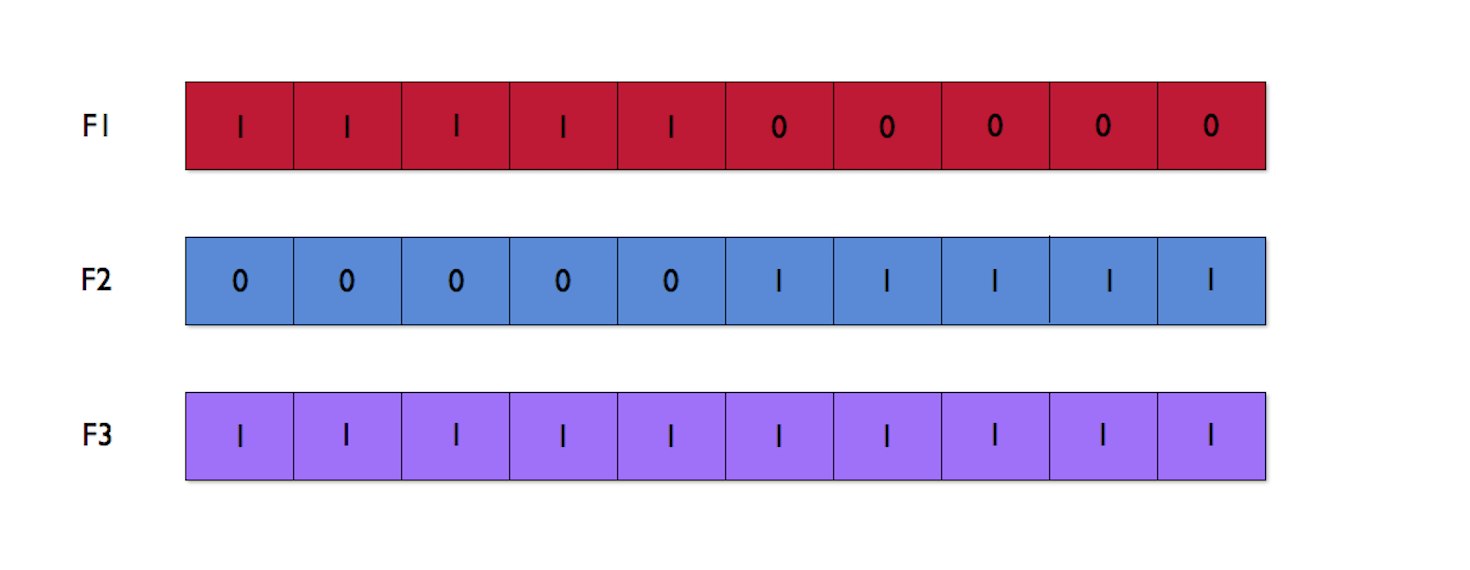
\includegraphics[width=1.0\textwidth]{pictures/filters.png}\\
  \caption[Jaccard-Distanzen zwischen Bloom-Filtern]{Jaccard-Distanzen zwischen Bloom-Filtern.}\label{fig:pic1}
\end{figure}
\noindent
Die Jaccard-Distanzen zwischen \textit{F1}, \textit{F2} und \textit{F3} betragen: 
\[J_{\delta}(F1,F3) = 1 - J(F1,F3) = 1 - \frac{|F1\cap F3|}{|F1\cup F3|} = 1 - \frac{5}{10} = 0.5\]
\[J_{\delta}(F2,F3) = 1 - J(F2,F3) = 1 - \frac{|F2\cap F3|}{|F2\cup F3|} = 1 - \frac{5}{10} = 0.5\]
\[J_{\delta}(F1,F2) = 1 - J(F1,F2) = 1 - \frac{|F1\cap F2|}{|F1\cup F2|} = 1 - 0 = 1\]
Daran wird deutlich: Obwohl \textit{F1} und \textit{F2} jeweils die Hälfte der Elemente mit \textit{F3} gemeinsam haben, lässt sich daraus kein Wert für die Ähnlichkeit zwischen \textit{F1} und \textit{F2} ableiten. Sie sind sich im Gegenteil maximal unähnlich. 
\subsection{Teil- und Obermengenbeziehung}\label{sec:mengenbeziehungen}
Will man Bloom-Filter z.B. nach Ähnlichkeit gruppieren, kann man stattdessen Teil- und Obermengenbeziehungen zwischen ihnen betrachten. Die Teilmengenbeziehung zwischen zwei Bloom-Filtern sei hier wie folgt definiert: 
\begin{quote}
Ein Bloom-Filter \textit{F} ist \textit{Teilmenge} eines Bloom-Filters \textit{G}, wenn darin mindestens die gleichen 0-Bits gesetzt sind wie in \textit{G} (und möglicherweise weitere, zusätzliche 0-Bits).
\end{quote}
Die Obermengenbeziehung zwischen zwei Bloom-Filtern sei hier wie folgt definiert: 
\begin{quote}
Ein Bloom-Filter \textit{F} ist \textit{Obermenge} eines Bloom-Filters \textit{G}, wenn darin mindestens die gleichen 1-Bits gesetzt sind wie in \textit{G} (und möglicherweise weitere, zusätzliche 1-Bits).
\end{quote}
Der maximal gefüllte Filter, in dem alle Bits gesetzt sind, ist damit Obermenge aller Filter derselben Länge (auch von sich selbst). Der leere Filter ist die (triviale) Teilmenge aller Filter derselben Länge (auch von sich selbst). Teil- und Obermengen sind Umkehrungen voneinander, d.h. wenn \textit{F} Teilmenge von \textit{G} ist, folgt daraus, dass \textit{G} Obermenge von \textit{F} ist, und umgekehrt.  

Zwischen den Bloom-Filtern in Abbildung \ref{fig:pic1} bestehen folgende Teil- und Obermengenbeziehungen: \textit{F1} und \textit{F2} sind Teilmengen von \textit{F3}. \textit{F3} ist Obermenge von \textit{F1} und \textit{F2}. Zwischen den maximal unähnlichen Filtern \textit{F1} und \textit{F2} bestehen keine Teil- und Obermengenbeziehungen. 
\begin{figure}[hpbt]
  \centering
  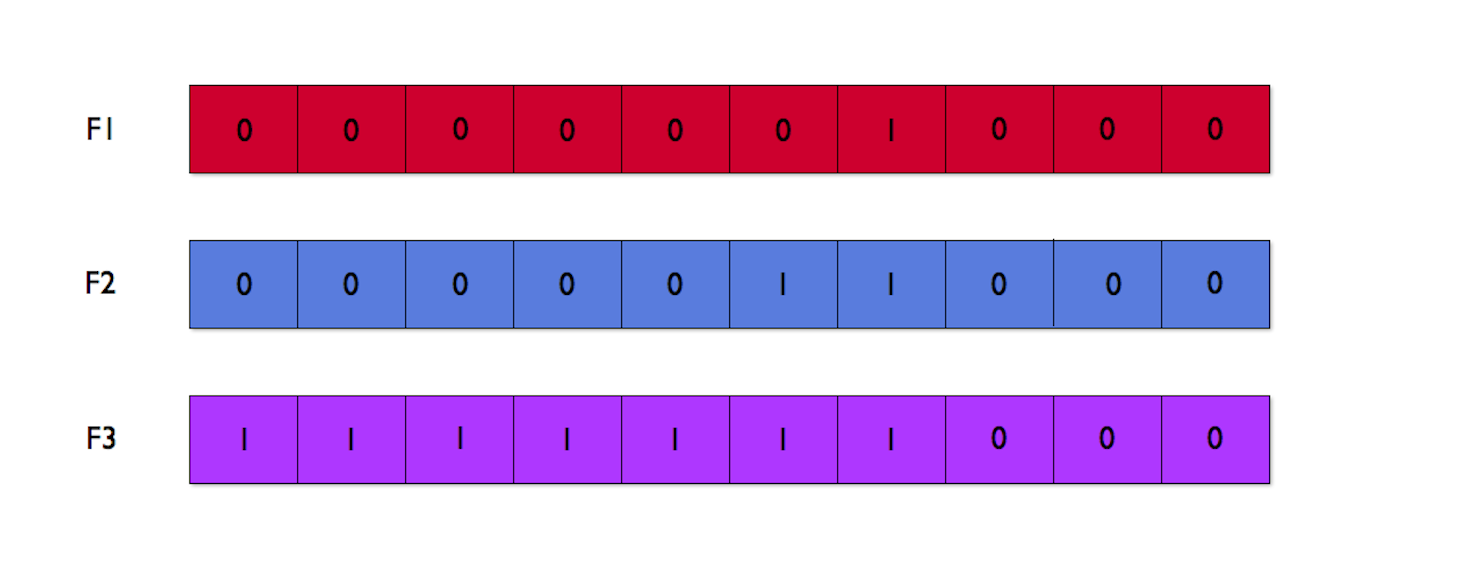
\includegraphics[width=1.0\textwidth]{pictures/distances.png}\\
  \caption[Teil- und Obermengenbeziehungen zwischen Bloom-Filtern]{Teil- und Obermengenbeziehungen zwischen Bloom-Filtern.}\label{fig:pic2}
\end{figure}

\noindent
Teil- und Obermengenbeziehung sind außerdem transitiv, was an Abbildung \ref{fig:pic2} deutlich wird: \textit{F1} ist Teilmenge von \textit{F2}, damit auch Teilmenge von \textit{F3}. \textit{F3} ist Obermenge von \textit{F2}, damit auch Obermenge von \textit{F1}. 

Teil- und Obermengenbeziehungen sind also im Gegensatz zur Jaccard-Distanz dazu geeignet, transitive Ähnlichkeitsbeziehungen zwischen Bloom-Filtern abzubilden. Diese Eigenschaft spielt eine zentrale Rolle im hier entwickelten Verfahren, das in Kapitel \ref{ch:implementierung} ausführlich dargestellt wird. 
\subsection{Hashfunktionen}\label{sec:hashfunktionen}
Zum Einfügen von Objekten in einen Bloom-Filter werden \textit{k} unabhängige Hashfunktionen $h_1,\ldots , h_k$ mit Wertebereich $\{ 0,\ldots, m-1\}$ verwendet, wobei \textit{m} die Größe des Bloom-Filters bezeichnet. Dabei wird davon ausgegangen, dass diese Hashfunktionen jedem Objekt im Universum einen zufälligen Hashwert aus dem Bereich $\{ 0,\ldots, m-1\}$ zuweisen, und dass diese Werte einer Gleichverteilung folgen \cite{Mitzenmacher2002}. Die optimale Anzahl an Hashfunktionen, die zur Minimierung der Falsch-Positiv-Rate benötigt wird, lässt sich in Abhängigkeit von den Parametern \textit{m}, \textit{n} und \textit{f} berechnen. Hierbei bezeichnet \textit{m} die Filtergröße, \textit{n} die Anzahl der erwarteten einzufügenden Objekte und \textit{f} die maximal akzeptierte Falsch-Positiv-Rate. Damit lässt sich die Anzahl benötigter Bits, d.h. die Filtergröße, berechnen als
\[m = -n\ast ln(f) / (ln(2)^2).\]
Hat man die Filtergröße bestimmt, lässt sich die Anzahl benötigter Hashfunktionen berechnen als 
\[d = \Ceil[\Bigg]{\frac{m}{n}\ast ln(2)}.\]
Die Frage nach den idealen Hashfunktionen für einen Bloom-Filter ist nicht eindeutig zu beantworten \cite{Broder2004}. Grundsätzlich muss zwischen kryptografischen Hashfunktionen wie MD5 und SHA und gewöhnlichen Hashfunktionen wie Murmur- oder Jenkins-Hashfunktionen unterschieden werden. Die Berechnung von kryptografischen Hashfunktionen dauert in der Regel länger, dafür haben sie bestimmte Eigenschaften wie eine hohe Kollisionsresistenz und Gleichverteilung der Ergebniswerte. 

Werden Bloom-Filter z.B. zum schnellen Nachschlagen in großen, verteilten Datenbanken eingesetzt, wird auf die kryptografischen Eigenschaften zu Gunsten des verminderten Rechenaufwandes verzichtet. Das NoSQL-Datenbanksystem Cassandra und das Hadoop-Framework für skalierte, verteilt arbeitende Software verwenden beispielsweise Bloom-Filter in Kombination mit Murmur- und Jenkins-Hashfunktionen. Darüber hinaus ist MD5 für Bloom-Filter weit verbreitet. Murmur-Hashfunktionen haben gute Verteilungseigenschaften und lassen sich vergleichsweise schnell berechnen, weswegen sie generell für den Einsatz in Bloom-Filtern empfohlen werden\footnote{Vgl. \mbox{\url{http://spyced.blogspot.de/2009/01/all-you-ever-wanted-to-know-about.html} (17.07.2016).}}. AMBIENCE verwendet Murmur-Hashfunktionen zur Generierung der Bloom-Filter. Für die eigene Implementierung wurde der Murmur2-Hash verwendet\footnote{Vgl. \url{https://sites.google.com/site/murmurhash/MurmurHash2.cpp} (17.07.2016) für den Quellcode.}.  
\subsection{Bloom-Filter-Varianten und Anwendungen}\label{sec:bloom-anwendungen}
Wegen ihres geringen Speicherbedarfs und einfachen Implementierung erfreuen sich Bloom-Filter in unterschiedlichsten Versionen großer Beliebtheit. Wichtige Varianten sind z.B. \textit{Attenuated Bloom Filter}, \textit{Counting Bloom Filter} und \textit{Compressed Bloom Filter}. Ein Counting Bloom-Filter benötigt mehr Speicherplatz als ein klassischer Bloom-Filter, dafür können Objekte wieder daraus entfernt werden \cite{Fan2000}. Komprimierte Bloom-Filter werden eingesetzt, wenn Bloom-Filter als Nachrichten mit begrenzter Länge versendet werden oder die übertragene Datenmenge minimiert werden soll \cite{Mitzenmacher2002}. Attenuated Bloom-Filter \cite{Sakuma2011} können als Array von Bloom-Filtern betrachtet werden und können z.B. in einem Netzwerk Informationen darüber enthalten, welche Dienste an einem anderen Knoten verfügbar sind. Besonders häufig kommen Bloom-Filter in verteilten Anwendungen und Netzwerkdiensten zum Einsatz \cite{Broder2004}. 

Neben Hadoop und Cassandra werden Bloom-Filter in unzähligen, zum Teil hoch skalierenden Anwendungen eingesetzt. Weitere Beispiele sind der quelloffene Webproxy Squid und der Chrome-Browser, wo Bloom-Filter zum schnellen Nachschlagen von als bösartig eingestuften URLs verwendet werden. Broder und Mitzenmacher formulieren das Bloom-Filter-Prinzip wie folgt: 
\begin{quote}
\textit{"`Wherever a list or set is used, and space is at a premium, consider using a Bloom filter if the effect of false positives can be mitigated."'} \cite{Broder2004}
\end{quote}
\section{Indexstrukturen}\label
Zur effizienten Bearbeitung von Anfragen und Operationen kommen in der internen Schicht von Datenbanksystemen spezielle Datenstrukturen und Speicherverfahren zum Einsatz. Sie werden \textit{Indexstrukturen} genannt und organisieren die Daten an Hand von Indizes, um die gewünschten Operationen zu unterstützen.\footnote{Trotz der großen Verbreitung von Indexstrukturen in Datenbanksystemen scheinen in der Literatur keine überblicksartigen Darstellungen zu existieren. Der aktuelle Abschnitt stützt sich daher im Wesentlichen auf das Skript zur Vorlesung \textit{Anfragebearbeitung und Indexstrukturen in Datenbanksystemen} im Wintersemester 2013/2014 an der Ludwig-Maximilians-Universität München \cite{Kriegel1994--2013}.}

Ein \textit{Index} oder \textit{Verzeichnis} einer Datei enthält Informationen über ihre Struktur, wobei mit "`Datei"' in diesem Zusammenhang eine komplette Datenstruktur gemeint ist, also z.B. ein Suchbaum oder ein Array. Den Datensätzen werden dabei meist Schlüssel oder IDs zugewiesen, an Hand derer sie in der Indexstruktur organisiert und gesucht werden. D.h. nicht die Datensätze selbst werden einer einer bestimmten Ordnung zu Folge organisiert, sondern lediglich ihre Schlüssel. Eine Anfrage nach einem Datensatz ermittelt dann zunächst den zugehörigen Schlüssel, sucht dessen Position in der Indexstruktur und greift erst dann auf den tatsächlichen Datensatz zu, wenn seine Position z.B. auf dem Plattenspeicher ermittelt wurde. Indexstrukturen lassen sich danach klassifizieren, wie sie die Daten organisieren: 
\begin{enumerate}
\setlength{\itemsep}{20pt}
	\item \textit{Daten-organisierende Indexstrukturen} werden zur Organisation der tatsächlich anfallenden Daten eingesetzt -- meist in Form von \textit{Suchbäumen}. 
	\item \textit{Raum-organisierende Indexstrukturen} werden zur Organisation des Speichers eingesetzt, in dem die Daten gehalten werden. Sie verwenden vor allem \textit{dynamische Hashverfahren}. 
	\item \textit{Hybride Indexstrukturen} sind eine Kombination der vorgenannten Klassen und basieren auf \textit{Hashbäumen}.   
\end{enumerate}
% \enlargethispage{2\baselineskip}
Eine gute bzw. effektive Indexstruktur sollte folgenden Anforderungen genügen: 
\begin{enumerate}
\setlength{\itemsep}{20pt}
	\item \textit{Effiziente Suche:} Eine Suchanfrage auf der Indexstruktur soll in optimaler Zeit ein Ergebnis liefern. D.h. die Anfrage soll in möglichst wenigen Schritten an die Seite oder Seiten weiter geleitet werden, die die angefragten Daten enthalten.
	\item \textit{Dynamisches Einfügen, Modifizieren und Löschen von Datensätzen:} Die zu organisierende Datenmenge verändert sich möglicherweise über die Zeit, was durch die Indexstruktur widergespiegelt und unterstützt werden muss.  
	\item \textit{Erhalt der lokalen Ordnung:} Falls es Datensätze gibt, deren Schlüssel in der angewandten Ordnungsrelation (z.B. die Kleiner-Gleich-Ordnung) aufeinander folgen, sollte die Indexstruktur diese Ordnung übernehmen. Suchbäumen erfüllen diese Eigenschaft, nicht aber lineare Hashverfahren. Die Wahl bzw. Implementierung der Indexstruktur muss also zum Anwendungsfall passen. 
	\item \textit{Speichereffizienz:} Effiziente Speichernutzung ist für real existierende und hoch skalierende Anwendungen von zentraler Bedeutung. 
\end{enumerate}
Weitere mögliche Anforderungen sind \textit{Machbarkeit} und \textit{Implementierungskosten}. Sie sind für die vorgestellte Implementierung nachrangig in dem Sinne, dass der Nachweis der Machbarkeit durch die Implementierung selbst erfolgt. Da AMBIENCE ein Prototyp ist und im akademischen Umfeld entwickelt wurde, kann die wirtschaftliche Kalkulation der Kosten, wie sie ein Unternehmen vornehmen würde, außer Acht gelassen werden. 

Für Implementierung (vgl. Kapitel \ref{ch:implementierung}) und Evaluation (vgl. Kapitel \ref{ch:evaluation}) stehen daher die Anforderungen 1--4 im Mittelpunkt. Als weiteres Kriterium, das nicht zu den allgemeinen Anforderungen an Indexstrukturen zählt, wurden die Aufbaukosten der Indexstruktur betrachtet. 
\subsection{B-Bäume}\label{sec:b-bäume}
B-Bäume sind eine weit verbreitete Form der Suchbäume und wurden zuerst 1972 von Rudolf Bayer und Edward M. McCreight vorgestellt. Sie erfüllen unter anderem folgende Eigenschaften:  
\begin{enumerate}
\setlength{\itemsep}{20pt}
	\item \textit{Aufbau:} B- und B$^+$-Bäume wachsen und schrumpfen von der Wurzel ausgehend.
	\item \textit{Balanciertheit:} Alle Blätter sind auf demselben Level. 
	\item \textit{Minimaler Grad/Ordnung:} B- und B$^+$-Bäume sind definiert durch die Ordnung oder den minimalen Grad \textit{t}, d.h. jeder Knoten außer der Wurzel enthält mindestens \textit{t} Schlüssel. 
	\item \textit{Suchbaumeigenschaft:} Schlüssel sind aufsteigend sortiert.
	\item \textit{Verzweigungsgrad:} Ein innerer Knoten mit \textit{k} Schlüsseln hat genau \textit{k+1} Kinder \cite{Ottmann2012}. Den Grad bzw. die minimale Ordnung betreffend ist die Nomenklatur in der Literatur uneinheitlich. Ottmann und Widmeyer \cite{Ottmann2012} sprechen in sprechen in Anlehnung an Knuth \cite{Knuth1999} von B-Bäumen der Ordnung \textit{m} und fordern, dass jeder Knoten mit Ausnahme der Wurzel und der Blätter mindestens $\lceil\frac{m}{2}\rceil$ Schlüssel enthalte. Stein et al. definieren den minimalen Grad wie weiter oben beschrieben \cite{Stein2009}, Kriegel verwendet dasselbe Kriterium, bezeichnet es jedoch als Grad \textit{m} \cite{Kriegel1994--2013}.
\end{enumerate}	
Abbildung \ref{fig:pic3} zeigt einen B-Baum der Ordnung 2, in den die Schlüssel \textbf{A--G}, \textbf{I--M}, \textbf{O--T}, \textbf{V--X} und \textbf{Z} eingefügt wurden. Ordnung 2 bedeutet: Die Wurzel muss mindestens einen Schlüssel enthalten, in diesem Fall den Wert \textbf{K}. Jeder innere Knoten und jedes Blatt enthält mindestens zwei Schlüssel. Der Verzweigungsgrad eines inneren Knotens ist um eins größer als die Anzahl seiner Schlüssel, z.B. hat die Wurzel einen Schlüssel und zwei Kindknoten. Alle Blätter sind auf demselben Level, in diesem Fall auf Level 3. Die Suchbaumeigenschaft ist erfüllt, d.h. der Schlüssel mit dem lexikografisch kleinsten Wert \textbf{A} ist am weitesten links, der Schlüssel mit dem lexikografisch größten Wert \textbf{Z} ist am weitesten rechts im Baum zu finden. 
\begin{figure}[hpbt]
  \centering
  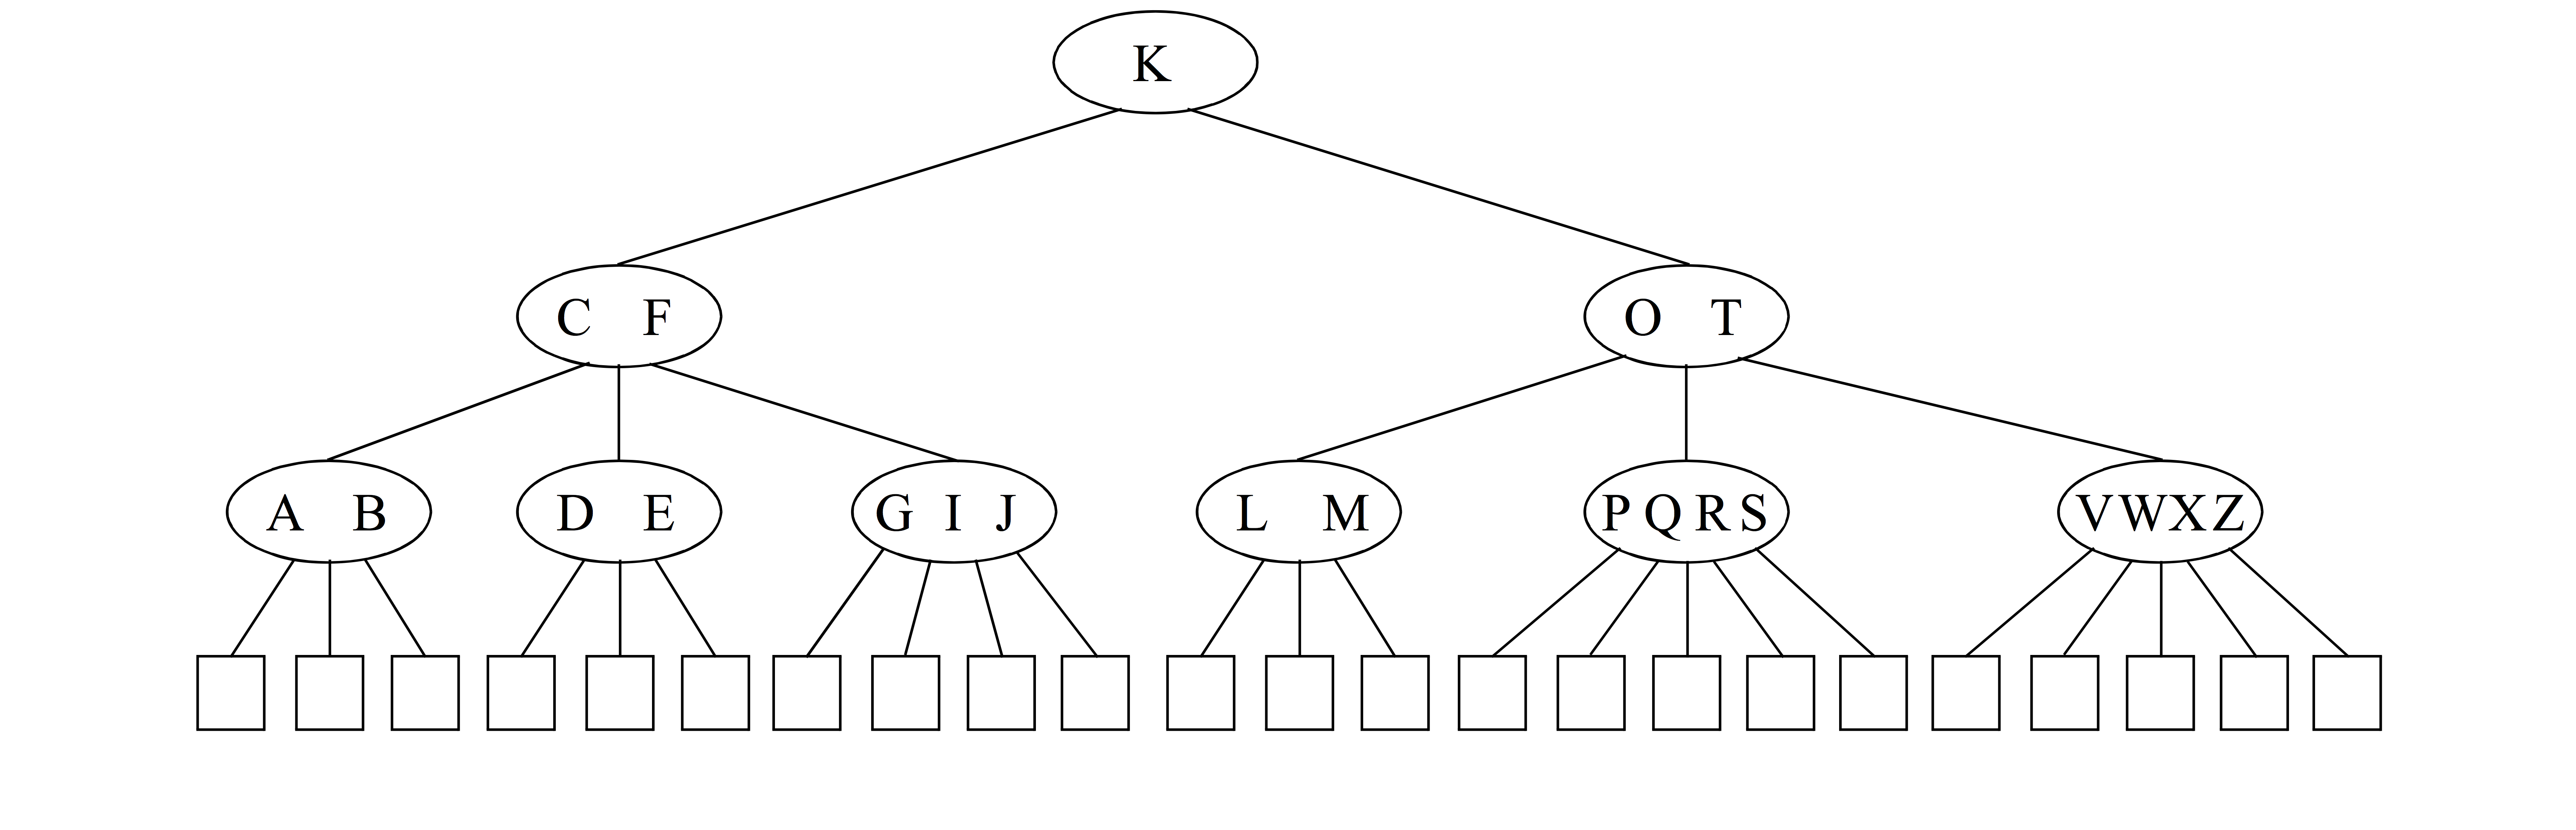
\includegraphics[width=1.0\textwidth]{pictures/b-baum.png}\\
  \caption[Ein B-Baum der Ordnung 2]{Ein B-Baum der Ordnung 2 \cite{Kriegel1994--2013}.}\label{fig:pic3}
\end{figure}
Unterstützte Operationen sind in der Regel Einfügen, Suchen und Löschen von Datensätzen. Dabei ist die Löschoperation am aufwendigsten zu implementieren, da auch das Löschen eines Schlüssels aus einem inneren Knoten betrachtet werden muss. Ein Schlüssel aus einem inneren Knoten kann nicht direkt gelöscht werden, da er zusätzlich als Separator für seine Kindknoten dient. Es muss daher ein neuer Separator aus dem rechten oder linken Kindknoten entnommen und in den Knoten eingefügt werden. Falls damit die B-Baum-Eigenschaften verletzt werden, d.h. der Kindknoten anschließend zu wenig Schlüssel enthält, muss eine Underflow-Behandlung eingeleitet werden, bei dem der Kindknoten mit einem Geschwisterknoten verschmolzen wird. Der Underflow kann sich rekursiv bis zur Wurzel fortsetzen und dafür sorgen, dass der Baum eine Ebene verliert und eine neue Wurzel erhält. 
\subsection{B$^+$-Bäume}\label{sec:b+bäume}
Das entwickelte Verfahren stützt sich stark auf \textit{B$^+$-Bäume}, eine Erweiterung der B-Bäume. Sie unterscheiden sich von ihnen in folgenden Eigenschaften: 
\begin{enumerate}
\setlength{\itemsep}{20pt}
	\item \textit{Minimale Schlüsselanzahl:} Jeder innere Knoten enthält mindestens einen Schlüssel.  
	\item \textit{Ordnungsrelation:} Der Kindknoten zwischen den Schlüsseln \textit{k1} und \textit{k2} enthält alle Schlüssel $\geq$ \textit{k1} und < \textit{k2}.
	\item \textit{Speicherung der Datensätze:} Alle Schlüssel werden auch in den Blättern gespeichert. Die tatsächlichen Datensätze sind mit dem entsprechen Schlüssel im Blatt verknüpft. 
	\item \textit{Sequentielle Verkettung:} Alle Blätter sind gemäß der Ordnung auf den Primärschlüsseln verkettet. 
\end{enumerate}
Abbildung \ref{fig:pic4} zeigt einen B$^+$-Baum der Ordnung 2, in den die Schlüssel \textbf{An}, \textbf{And}, \textbf{Certain}, \textbf{For}, \textbf{From}, \textbf{Which} und \textbf{With} eingefügt wurden. Ordnung 2 bedeutet in diesem Fall: Die Wurzel muss mindestens einen Schlüssel enthalten, in diesem Fall den Wert \textbf{For}. Jeder innere Knoten enthält mindestens einen und jedes Blatt enthält mindestens zwei Schlüssel. Der Verzweigungsgrad eines inneren Knotens ist um eins größer als die Anzahl seiner Schlüssel, z.B. hat die Wurzel einen Schlüssel und zwei Kindknoten. Alle Blätter sind auf demselben Level, in diesem Fall auf Level 3.

Die inneren Baumknoten erfüllen die Ordnungsrelation \textit{k1} < Kindknoten-Schlüssel $\leq$ \textit{k2}. Z.B. enthält der Blattknoten ganz links alle Schlüssel, deren Wert lexikografisch kleiner ist als der \textbf{Certain} im Elternknoten. Der zweite Blattknoten enthält alle Schlüssel, deren Wert lexikografisch $\geq$ \textbf{Certain} ist und zudem kleiner als \textbf{For}, den Schlüssel im Wurzelknoten, da die Ordnungsrelation natürlich im ganzen Baum erfüllt sein muss. Alle Datensätze sind auch in den Blättern gespeichert, z.B. findet sich der Schlüssel \textbf{For} sowohl in der Wurzel als auch im dritten Blattknoten. Darin unterscheidet sich der B$^+$-Baum vom B-Baum. Dort ist der Schlüssel \textbf{K} z.B. nur in der Wurzel abgespeichert, nicht aber im Blattknoten (vgl. Abbildung \ref{fig:pic3}).  
\begin{figure}[hpbt]
  \centering
  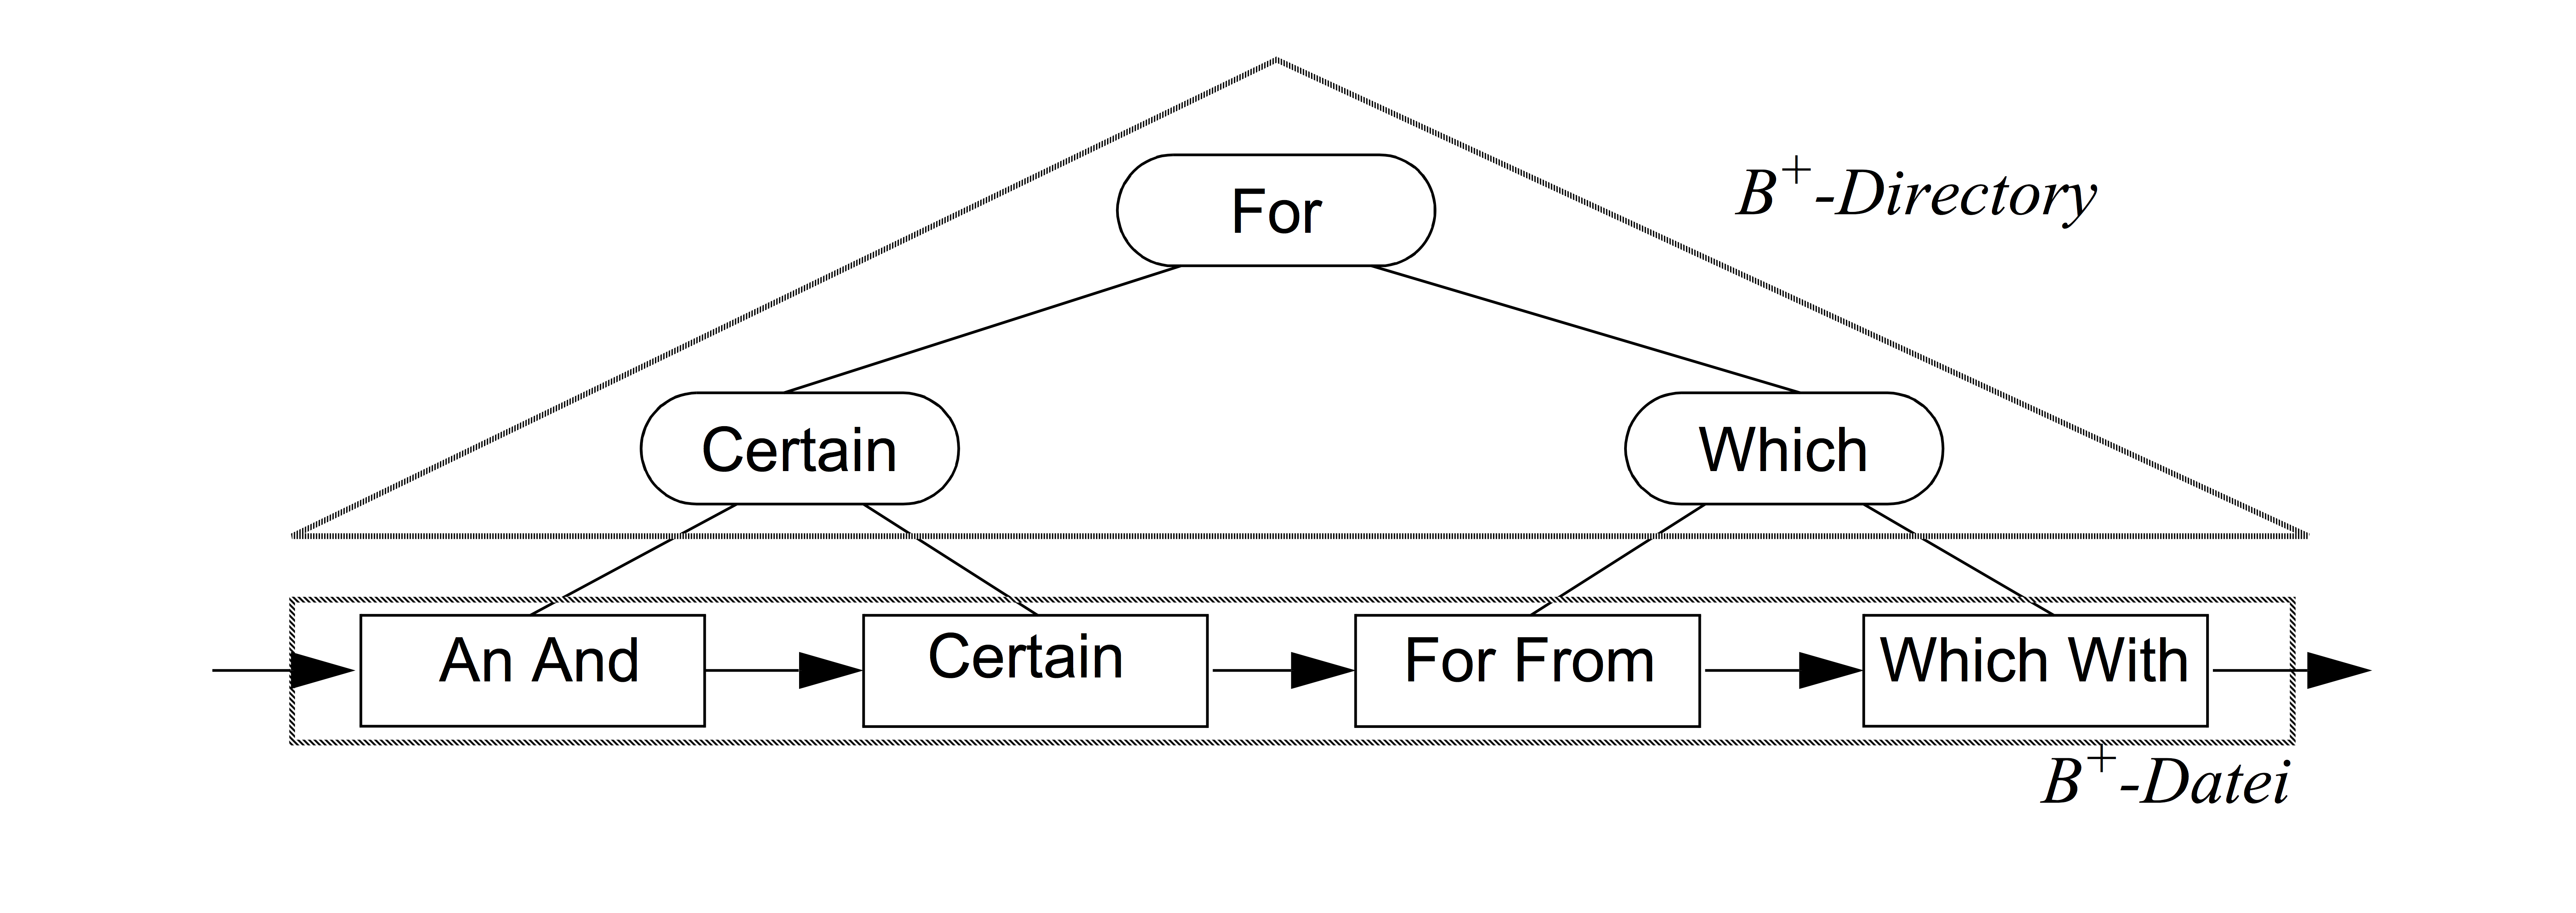
\includegraphics[width=1.0\textwidth]{pictures/b+baum.png}\\
  \caption[Ein B$^+$-Baum der Ordnung 2]{Ein B$^+$-Baum der Ordnung 2 \cite{Kriegel1994--2013}.}\label{fig:pic4}
\end{figure}
\noindent
Alle Blätter sind gemäß der Ordungsrelation verkettet, was durch die Pfeile auf Level 3 symbolisiert wird. Dieser B$^+$-Baum ermöglicht damit z.B. eine Bereichsanfrage vom Typ "`Lies die Informationen aller Datensätze im Bereich von \textbf{And} bis \textbf{For} aus"'. Dazu genügt es, einmal den Schlüssel \textbf{And} im Baum zu suchen und von dort aus den Zeigern auf der Blattebene zu folgen, bis entweder der Schlüssel \textbf{For} oder, wenn dieser nicht im Baum enthalten ist, ein Schlüssel mit einem lexikografisch größeren Wert erreicht ist. Solch eine Anfrage ist im B-Baum aus Abbildung \ref{fig:pic3} nicht möglich. Dort benötigt eine Anfrage nach allen Schlüsseln im Bereich von \textbf{B} bis \textbf{V} sechs rekursive Suchaufrufe, da es keine Möglichkeit gibt, die Nachbarknoten auf Blattebene zu erreichen. 
 
Neben der Bereichssuche zählt der höhere Verzweigungsgrad zu den wesentlichen Vorteilen des B$^+$-Baums gegenüber dem B-Baum. Tabelle \ref{tab:Trees} vergleicht die durchschnittlichen Laufzeiten für Einfügen, Suchen und Löschen in B-Bäumen und B$^+$-Bäumen.
\begin{center}
\begin{table}[htbp]
{\small
\begin{center}
\begin{tabular}[center]{lcccc}
\toprule
 & \textbf{Einfügen} & \textbf{Suchen} & \textbf{Löschen} & \textbf{Bereichssuche}\\
\midrule
\textbf{B-Baum} & $O(log (2t -1))$ & $O(log (2t -1))$ & $O(log (2t -1))$ & $\times$ \\
\midrule
\textbf{B$^+$-Baum} & $O(log (2t -1))$ & $O(log (2t -1))$ & $O(log (2t -1))$ & $O(log 2t-1)$\\
\bottomrule
\end{tabular}
\end{center}
} % end of tiny
\caption[Laufzeiten von Operationen auf Suchbäumen]{Laufzeiten von Operationen auf Suchbäumen.\label{tab:Trees}}
\end{table}
\end{center}
Daran wird deutlich, dass die Kosten für Einfügen, Suchen und Löschen in beiden Varianten vom Parameter \textit{t} abhängen. Da die inneren Knoten im B$^+$-Baum mehr Schlüssel enthalten als im B-Baum, wird der Baum breiter und flacher. Geht man davon aus, dass ein Zugriff auf einen inneren Knoten einem Plattenzugriff entspricht, wird deutlich, dass sich damit die Kosten für Einfügen, Suchen und Löschen gegenüber dem B-Baum reduzieren lassen.

Die sequentielle Verkettung der Blätter im B$^+$-Baum ermöglicht zudem eine Bereichssuche. Das ist ein immenser Vorteil gegenüber dem B-Baum, bei dem jeder für eine Bereichssuche jeder einzelne Datensatz mit Kosten von $O(log (2t -1))$ gesucht werden muss. Diese Kosten fallen beim B$^+$-Baum nur für den ersten Datensatz mit dem kleinsten Primärschlüssel an. Anschließend kann eine doppelt verkettete Liste traversiert werden.
    \chapter{Verwandte Themen}\label{ch:related}
\enlargethispage{2\baselineskip}
Im Netzwerk AMBIENCE, das als Schnittstelle für den eigenen Entwurf diente, spielen Bloom-Filter eine wichtige Rolle. Für die vorliegende Arbeit wurden Bloom-Filter implementiert, um eigene Berechnungen zu überprüfen und mit realistischen Werten arbeiten zu können. Das folgende Kapitel stellt in Abschnitt \ref{sec:bloom-implementierung} zunächst dar, auf welche Arbeiten und bewährten Techniken dabei Bezug genommen wurde.  

Ziel dieser Arbeit war eine optimale Lösung für das Anwendungsszenario von AMBIENCE. Eine solche wird vom aktuellen Stand der Forschung nicht abgedeckt. In den Abschnitten \ref{sec:mengenvergleich} sowie \ref{sec:organisation} wird zunächst allgemein auf den Mengenvergleich mit Bloom-Filtern und die Organisation von Mengen von Bloom-Filtern eingegangen. Die Darstellung des aktuellen Forschungsstandes konzentriert sich auf Bloom-Filter in Netzwerkanwendungen und Indexstrukturen sowie die \textit{k}-nächste-Nachbarn-Suche. Überlegungen und Arbeiten, die Eingang in die eigene Implementierung gefunden haben, werden in den Abschnitten \ref{sec:bloom-netzwerk}, \ref{sec:bloom-index} und \ref{sec:bloom-knn} vorgestellt. 
\section{Einsatz von Bloom-Filtern}\label{sec:bloom-implementierung}
Gemäß dem Bloom-Filter-Prinzip bietet sich die Verwendung von Bloom-Filtern an, wenn Speicherplatz effektiv genutzt werden soll und gleichzeitig die Auswirkungen von falsch positiven Ergebnissen abgemildert werden können (vgl. Abschnitt \ref{sec:bloom-anwendungen}). Die mathematischen Grundlagen wie Minimierung der Falsch-Positiv-Rate, Abschätzung der Anzahl eingefügter Elemente, Abschätzung der Jaccard-Distanz etc. werden beispielsweise von Bloom \cite{Bloom1970}, Broder \cite{Broder2004}, Mitzenmacher \cite{Mitzenmacher2002} sowie Werner et al. \cite{Werner2015} ausführlich dargestellt. 

Wie in den Abschnitten \ref{sec:hashfunktionen} und \ref{sec:bloom-anwendungen} erwähnt, werden Bloom-Filter im Apache-Projekt Cassandra eingesetzt. Sie dienen dort zum schnellen Nachschlagen in Tabellen, den so genannten \textit{SSTables}. Die Cassandra-Entwickler, namentlich Jonathan Ellis, haben sich eingehend mit der Implementierung von Bloom-Filtern und optimalen Hashfunktionen beschäftigt. Diese Überlegungen haben keinen Eingang in wissenschaftliche Veröffentlichungen gefunden, sind jedoch sehr praxisrelevant.\footnote{Die Hauptseite des Cassandra-Projekts ist unter \url{http://cassandra.apache.org/} (17.07.2016) zu finden. Der Cassandra-Quellcode ist frei verfügbar unter \url{https://github.com/apache/cassandra} (17.07.2016). Datenmodell und Architektur werden z.B. unter \url{http://wiki.apache.org/cassandra/DataModel} (17.06.2016), \url{http://wiki.apache.org/cassandra/ArchitectureOverview} (17.07.2016) und \url{http://prettyprint.me/prettyprint.me/2010/05/02/understanding-cassandra-code-base/index.html} (17.07.2016) beschrieben. Für diese Arbeit wurden auch eine programmatische Rede unter \url{https://youtu.be/WD1v6jr5fKY} (17.07.2016) und ein Blog unter \url{http://spyced.blogspot.de/} (17.07.2016) von Ellis berücksichtigt.} Zur Wahl der Hashfunktionen schreibt Ellis: 
% \newpage
\begin{quote}
\textit{"`[I]t turns out that it's surprisingly hard to find good information on one part of the implementation: how do you generate an indefinite number of hashes? Even small filters will use three or four; a dozen or more is not unheard of."'}\footnote{\mbox{\url{http://spyced.blogspot.de/2009/01/all-you-ever-wanted-to-know-about.html} (17.07.2016).}} 
\end{quote}
Die mathematischen Grundlagen der Generierung von \textit{i} Hashfunktionen mit möglichst gleich verteilten Ergebnissen sind bei Kirsch und Mitzenmacher zu finden \cite{Kirsch2006}. Viele Bloom-Filter-Implementierungen wie \textit{PyBloom} verwenden jedoch Hashfunktionen, deren Ergebnisse nicht gleich verteilt sind. Das Problem ist, dass damit häufig eine deutlich höhere Falsch-Positiv-Rate im Bloom-Filter erzielt wird als rein rechnerisch zu erwarten wäre. 

Der Grund für die Verwendung minderwertiger Hashfunktionen ist Ellis zu Folge, dass die meisten Implementierungen auf schnelle Berechnung der Hashwerte abzielten statt auf Gleichverteilung der Ergebnisse. Das ist aber für einen Bloom-Filter essentiell, wenn z.B. wie in Cassandra teure Eingabe/Ausgabe-Operationen durch den Einsatz von Bloom-Filtern reduziert werden sollen. Weist der Bloom-Filter eine erhöhte Falsch-Positiv-Rate auf, beispielsweise von 140\% gegenüber dem erwarteten Wert, reduziert das die positiven Effekte des Bloom-Filters drastisch.  

Ellis präsentiert zwei Lösungsansätze: Entweder kryptografische Hashfunktionen oder Murmur- und Jenkins-Hashfunktionen mit guter Gleichverteilung der Ergebnisse. Kryptografische Hashfunktionen wurden bereits in Abschnitt \ref{sec:hashfunktionen} dargestellt. Der Nachteil daran ist, dass sie in der Regel aufwändiger zu berechnen sind als gewöhnliche Hashfunktionen. Das spielt z.B. bei der einmaligen Berechnung eines Fingerabdrucks keine große Rolle. Die Performanz von Bloom-Filtern wird dadurch aber beeinträchtigt. 

Mit Murmur- oder Jenkins-Hashfunktionen gibt es zwei Möglichkeiten, eine beliebige Anzahl von Hashfunktionen mit guter Gleichverteilung der Ergebnisse zu erzeugen. Entweder berechnet man den \textit{i}-ten Hashwert als $\text{hash0 }+ i\ast \text{hash1}$ wie von Kirsch und Mitzenmacher beschrieben und in Cassandra angewendet. Alternativ nimmt man den \textit{i}-ten Hashwert als Startwert für die Berechnung des \textit{i+1}-ten Hashwerts. Dieser Ansatz wurde in Hadoop gewählt und wird auch hier verwendet. 

Zur Organisation der Bloom-Filter äußert sich Ellis ebenfalls, jedoch nur auf seinem Twitter-Account und ohne auf Details einzugehen: 
\begin{quote}
\textit{"`Rather than naively checking every Bloom Filter for the element, organize the BF in a hierarchy akin to B+ tree."'}\footnote{\url{https://twitter.com/spyced/status/707266703751651328} (17.07.2016).}
\end{quote}
Zwar ist hier offensichtlich von der Suche nach einem Element in einem Bloom-Filter die Rede, nicht nach einem Bloom-Filter selbst wie in AMBIENCE. Dennoch zeichnet sich ab, dass ein B$^+$-Baum als Indexstruktur für Bloom-Filter in Erwägung gezogen werden sollte. 

Damit sind die Gemeinsamkeiten zwischen Cassandra und AMBIENCE erschöpft. Cassandra ist zur Evaluation von AMBIENCE nicht geeignet, da in AMBIENCE die Bloom-Filter selbst die Datensätze sind, während sie in Cassandra zum Nachschlagen der Datensätze verwendet werden. Die Publikationen aus dem Cassandra-Umfeld wurden daher ausschließlich bezüglich Implementierung der Bloom-Filter, Wahl und Berechnung der Hashfunktionen berücksichtigt. Der Hinweis auf B$^+$-Bäume in Zusammenhang mit Bloom-Filtern unterstützte zudem die Entscheidung für diese Indexstruktur. 
\section{Mengenvergleich}\label{sec:mengenvergleich}
Generell lassen sich beim Vergleich von Mengen zwei Ansätze unterscheiden: Exakte Berechnung der Mengendifferenz und Approximation. Die exakte Berechnung liefert dabei optimale Ergebnisse, ist aber mit deutlich höherem Rechenaufwand verbunden. Das kann für bestimmte Anwendungsfälle notwendig sein, etwa in der Medizin oder Biologie, wenn man falsch positive und falsch negative Ergebnisse eines Mengenvergleichs unter allen Umständen ausschließen möchte, z.B. bei der Diagnosestellung \cite{Schnell2013}. 

Oft wird jedoch auf eine Approximation von Mengendifferenzen zurückgegriffen, um den Rechenaufwand in einem überschaubaren Rahmen zu halten. Das gilt besonders bei der Verwendung großer Datensätze, hoch skalierenden oder auf Schnelligkeit angewiesenen Anwendungen. Besonders wichtig ist die Reduzierung des Rechenaufwands beim Vergleich von Mengen auf unterschiedlichen Hosts in einem Netzwerk. 

Approximation der Anzahl von Mengendifferenzen auf unterschiedlichen Hosts mit minimaler Kommunikation wird z.B. von Agarwal und Trachtenberg behandelt \cite{Agarwal2006}. Dort wird gezeigt, dass zur Lösung dieses Problems in etwa so viel Kommunikation notwendig ist wie zur Bestimmung der Differenzen selbst. Die Autoren haben hierzu eine heuristische Lösung basierend auf dem Counting Bloom-Filter entwickeltl, mit der sich bessere Ergebnisse bezüglich minimaler Kommunikation und minimaler Anzahl an Mengenvergleichen erzielen lassen als mit bestehenden Methoden. Solch eine Lösung kann z.B. in einem \textit{Content Delivery Network} (CDN) zur Anwendung kommen, wo es besonders wichtig ist, regelmäßig die existierenden Kopien von Datensätzen abzugleichen (vgl. hierzu auch \cite{Byers2002}). 

Der Kern der Anwendung liegt im so genannten Wrapping-Prozess. \textit{"`Wrapped filters"'} \cite{Agarwal2006} werden ähnlich wie Bloom-Filter konstruiert, indem zunächst alle Elemente des Bloom-Filters mit 0 initialisiert werden (vgl. Abschnitt \ref{sec:bloom}). Die einzufügenden Objekte, d.h. die Elemente der Menge, werden wie im Standard-Bloom-Filter mit Hilfe von \textit{k} unabhängigen Hashfunktionen eingefügt. Im Unterschied dazu können die Array-Elemente nicht nur Werte aus $\{0,1\}$ annehmen, sondern werden wie beim Counting Bloom-Filter inkrementiert. Der Vorteil des Verfahrens zeigt sich beim Unwrapping-Prozess. Er wird ausgeführt, nachdem der Wrapped Filter von Host A an Host B übermittelt wurde, mit dem der Mengenvergleich erfolgen soll: 
\begin{quote}
\textit{"`Host A can use [the] Bloom filter property of a wrapped function to determine $|S_A - S_B|$ by inspecting B's wrapped filter $W_{S_B}$; [\dots] all elements of $S_A$ that do not fit the Bloom filter can be considered to be in $S_A - S_B$. [\dots] Conversely, the unwrapping algorithm [\dots] allows us to approximation $|S_B - S_A|$ from the same wrapped filter, giving an overall approximation for the mutual difference $|S_A\oplus S_B|$."'} \cite{Agarwal2006}
\end{quote}
Generell verhält sich der Kommunikationsaufwand zur Approximation von Mengendifferenzen proportional zur Anzahl der in den Mengen enthaltenen Elemente. Den Autoren gelingt es mit ihrem Verfahren jedoch, einerseits diesen Aufwand zu verringern, andererseits auch die Performanz gegenüber einem Standard-Bloom-Filter zu verbessern. Sie schreiben hierzu: 
\begin{quote}
\textit{"`[T]he standard Bloom filter and wrapped filter approaches are very similar for filter sizes that are large relative to hosts sets. For smaller filters, Bloom filters generally provide a lower (and less accurate) approximation than wrapped filters [\dots]. Random sampling [\dots] is quite inaccurate unless almost all the samples are transmitted; both minwise sketches and random sampling have a high standard deviation compared to Bloom and wrapped filters."'} \cite{Agarwal2006}
\end{quote}
\section{Organisation von Mengen von Bloom-Filtern}\label{sec:organisation}
Eine Erweiterung der Arbeit von Agarwal und Trachtenberg wurde von Byers et al. 2002 vorgestellt mit dem Ziel einer
\begin{quote}
\textit{"`[\dots] collection of useful algorithmic tools for efficient summarization and approximate reconciliation of sets of symbols between pairs of collaborating peers, all of which keep message complexity and computation to a minimum."'} \cite{Byers2002}
\end{quote}
Die Autoren haben dazu eine neuartige Datenstruktur entwickelt, den \textit{Approximation Reconciliation Tree}, in dem \textit{Patricia-Tries}, \textit{Merkle-Bäume} und Bloom-Filter zusammengeführt werden. Der Name Patricia-Trie leitet sich vom Begriff \textit{information retrieval} ab, zu Deutsch etwa "`Informationsbeschaffung"'. Das Akronym PATRICIA steht für \textit{Practical Algorithm to Retrieve Information Coded In Alphanumeric}. Die Besonderheit des Patricia-Tries ist die komprimierte Speicherung von Datensätzen. Zeichen, für die kein Eintrag im Baum vorhanden ist, werden ausgelassen und die Anzahl der ausgelassenen Zeichen mit abgespeichert. Das hat den Vorteil, dass der Baum relativ langsam wächst, auch wenn große Anzahlen von neuen Schlüsseln eingefügt werden. 

Ein Merkle-Baum ist eine hybride Indexstruktur, in der ein Hashbaum zur Organisation der Daten dient (vgl. Abschnitt \ref{sec:index}). Jeder innere Baumknoten wird dabei mit dem Hashwert der Kindknoten markiert. Das ermöglicht die Überprüfung des Inhalts großer Datenstrukturen auf effiziente und -- abhängig von der Wahl der Hashfunktionen -- auch kryptografisch sichere Weise. 

Im Approximation Reconciliation Tree dienen Patricia-Tries zur strukturierten Suche basierend Teilmengenvergleichen. Zum Vergleich der Teilmengen werden Merkle-Bäume verwendet und schließlich Bloom-Filter zur kompakten Repräsentation eingesetzt. Der Approximation Reconciliation Tree wird also folgendermaßen: 
\begin{quote}
\textit{"`Each peer starts by building a Patricia trie of their set along with the associated Merkle tree values. The message A then sends to B is a Bloom filter of the values from the Merkle tree. For B to perform approximate reconciliation, B uses the same recursive algorithm previously used to traverse an uncollapsed trie, to traverse its collapsed Patricia trie $T_B$."'} \cite{Byers2002}
\end{quote}
Mit weiteren Verbesserungen wie einem erhöhten Verzweigungsgrad gelingt es den Autoren, mit dem Approximation Reconciliation Tree den approximativen Mengenvergleich gegenüber der Vergleichsimplementierung, die lediglich Bloom-Filtern verwendet, deutlich zu beschleunigen. Die Indexstruktur ist als Primitiv für Peer-to-Peer-Anwendungen gedacht, die als Form von kontextzentrischen Netzwerke verstanden werden können wie in Abschnitt \ref{sec:kontext} beschrieben. 
\section{Netzwerkanwendungen mit Bloom-Filtern}\label{sec:bloom-netzwerk}
Bloom-Filter werden in zahlreichen Netzwerk-Anwendungen eingesetzt. Das erscheint auf den ersten Blick interessant für AMBIENCE als soziales Online-Netz. Ein guter Überblick über Netzwerk-Anwendungen mit Bloom-Filtern findet sich in der Publikation von Broder und Mitzenmacher mit dem Ziel 
\begin{quote}
\textit{"`[...] to survey the ways in which Bloom filters have been used and modified in a variety of network problems, with the aim of providing a unified mathematical and practical framework for understanding them and stimulating their use in future applications."'} \cite{Broder2004}
\end{quote}
Die Autoren beschreiben unter anderem die Verwendung von Bloom-Filtern zur Kollaboration in Overlay- und Peer-to-Peer-Netzwerken, jedoch mit einem entscheidenden Unterschied zur Fragestellung: Zwar werden die Anfragen in AMBIENCE von einem mobilen Endgerät an einen Host gesendet, also über das Netzwerk übertragen. Die \textit{k}-nächste-Nachbarn-Suche bezieht sich jedoch auf die Menge der an einem Host gespeicherten Bloom-Filter. Unter diesen sollen die ähnlichsten möglichst schnell und effizient gefunden werden. Ab dem Zeitpunkt, zu dem die Anfrage am Host eingegangen ist, werden aber keine Nachrichten mehr im Netzwerk übertragen. Die \textit{k}-nächste-Nachbarn-Suche findet nur auf dem Host selbst statt und erst das Ergebnis wird an das anfragende Gerät übermittelt. 

Eine Anwendung von Bloom-Filtern in Verbindung mit Fingertabellen in Peer-to-Peer-Netzwerken wird von Shiraki et al. beschrieben \cite{Shiraki2009}. Die Autoren stellen eine Methode zur Suche von Nutzern basierend auf Bewegungsmeldungen vor, die als Sequenz von Paaren aus einer \textit{spot-ID} und einem Zeitstempel gespeichert werden. Alle diese Paare werden in einen Bloom-Filter eingefügt, der damit das Bewegungsverhalten eines Anwenders abbildet. Zudem wird eine \textit{Bloom Finger Table} eingeführt. Sie basiert auf dem strukturierten Peer-to-Peer-Protokollsystem Chord, in dem die effiziente Suche nach Inhalten über eine Fingertabelle erfolgt. Jedem eingefügten Datensatz im Netzwerk wird dabei über eine globale Hashfunktion eine eindeutige ID zugewiesen. Sie ist das Ergebnis der Berechnung einer SHA-Hashfunktion. Jeder Knoten im Netzwerk verwaltet einen Teil der globalen Hashtabelle. Knoten halten damit also selbst einen Teil der Daten wissen für einen anderen Teil, an welcher Stelle sie sich befinden. Die Einträge in der Fingertabelle werden erstellt, indem der \textit{i}-te Finger auf den Knoten verweist, der den Schlüssel mit dem Hashwert $x+2(i-1)$ verwaltet. Diese Struktur beschleunigt die Suche nach Schlüsseln bzw. Datensätzen gegenüber der linearen Suche deutlich. Eine Bloom Finger Table wird bei Shiraki et al. wie folgt gebildet: 
\begin{quote}
\textit{"`To search multiple elements, a combined Bloom Filter of the elements is generated. Then the query is forwarded to the peer in the Finger Table when the Bloom Filter of the query is included in the corresponding Bloom Filter. [\dots] If the Bloom Filter of the peer is included by the Bloom Filter of the query, the peer is matched to the query. However, all elements have to be tested again on the peer since the testing by Bloom Filter has false positive."' }\cite{Shiraki2009}
\end{quote}
Die Suche nach Nutzern basiert auf der Anwendung von bitweisem logischen Und bzw. Oder auf Bloom-Filtern wie in Abschnitt \ref{sec:distanzmasse} beschrieben. Das bitweise logische Und entspricht dabei einer Suchanfrage nach allen IDs der Teilnehmer, die \textit{alle} gesuchten \textit{Movement records}, d.h. Ort/Zeitstempel-Paare enthalten. Das bitweise logische Oder entspricht einer Anfrage nach allen IDs der Teilnehmer, die \textit{einen} der gesuchten \textit{Movement records} enthalten. Anfragen werden dabei gemäß den Bloom-Fingertabellen im Netzwerk weiter geleitet. Das Verfahren ermöglicht eine deutliche Reduzierung der Vergleiche bei der Suche nach Nutzern gegenüber der naiven Implementierung. 

Auch dieser spannende Ansatz ist leider nicht auf AMBIENCE übertragbar. Zum einen wird wie beschrieben mit der Und- bzw. Oder-Suche ein abweichendes Distanzmaß verwendet. Und obgleich es sich hier um ein Peer-to-Peer-Netzwerk handelt, das eher dem ICN-Ansatz als traditionellen Netzstrukturen zuzuordnen ist, unterscheidet sich das Konzept stark von AMBIENCE. Bei Shiraki et al. wird gezielt nach Nutzern gesucht und es werden ihre Bewegungsmeldungen aufgezeichnet. In AMBIENCE hingegen wird den Nutzern größtmögliche Anonymität gewährt, da das Netzwerk dezidiert kontext- und informationszentrisch strukturiert ist. 

Wie in Abschnitt \ref{sec:mengenvergleich} beschrieben, können Counting Bloom Filter dazu verwendet werden, um die Abschätzung von Mengendifferenzen auf unterschiedlichen Hosts zu optimieren. Daran werden die Vorteile von Bloom-Filtern bei der blinden Kalkulation von Mengenunterschieden deutlich, ohne dass ihre Elemente bzw. die Objekte in den Bloom-Filtern bekannt sein müssen. Wie bei Werner et al. beschrieben, kann diese Eigenschaft den Schutz der Privatsphäre in einem sozialen Online-Netz verbessern \cite{Werner2015}. Auch hier findet die Abschätzung der Mengendifferenzen jedoch zwischen zwei unterschiedlichen Hosts statt, weswegen dieser Ansatz für AMBIENCE nicht genutzt werden kann. Gleiches gilt für die Arbeiten von Byers et al. \cite{Byers2002}, Shiraki et al. \cite{Shiraki2009}, Zhang \cite{Zhang2012} und Zhu et al. \cite{Zhu2004}. Überall dort werden Bloom-Filter im Zusammenhang mit Netzwerken eingesetzt, doch keiner der Ansätze lässt sich auf AMBIENCE anwenden. 
\section{Indexstrukturen für Bloom-Filter}\label{sec:bloom-index}
Ein Überblick über Indexstrukturen für Datenbank-Managementsysteme auf Hauptspei\-cher\-basis findet sich bei Lehman und Carey \cite{Lehman1986}. Die Publikation kann zu einem besseren Verständnis der Indexstrukturen aus Abschnitt \ref{sec:index} beitragen. Wichtig ist vor allem die Erkenntnis, dass der Einsatz einer Hauptspeicher-Datenstruktur sinnvoll sein kann, um die Performanz von Anfragen auf größeren Datenmengen zu verbessern. B- und B$^+$-Bäume werden allgemein als Hauptspeicher-Datenstruk\-turen verwendet. Ein Vorteil davon ist die Reduzierung der Plattenzugriffe bei der Suche nach Datensätzen. In der Regel benötigen sie viel weniger Speicherplatz als das tatsächliche Datenaufkommen. Außerdem kann in der Indexstruktur häufig mit Zeigern gearbeitet werden, ohne alle vorhandenden Daten tatsächlich in der Datenstruktur halten zu müssen. Adaptierungen von kanonischen Formen der Indexstrukturen für spezifische Anwendungen finden sich vielfach in der Literatur. Wenig überraschend ist darunter keine, die das spezifische Szenario von AMBIENCE abbildet.

Hellerstein und Pfeffers Publikation von 1994 stellt den \textit{RD-Tree} als Indexstruktur für objektrelationale Geo-Datenbanken vor \cite{Hellerstein1994}. Abgesehen davon, dass der objektrelationale Ansatz mittlerweile kaum noch verfolgt wird, ist die Indexstruktur optimiert für Geodaten. Diese haben spezielle Eigenschaften wie z.B. Inklusionsbeziehungen zwischen Punkten und Flächen oder Flächen untereinander, die in der Indexstruktur abgebildet und von Suchanfragen unterstützt werden müssen. Spezielle Indexstrukturen für Geodaten erschienen daher ungeeignet, da sie einerseits einen unnötigen Implementierungsaufwand erfordern, andererseits die \textit{k}-nächste-Nachbarn-Suche unnötig erschweren. Zu diesen speziellen Indexstrukturen zählt auch der \textit{R-Baum} zur Organisation von minimalen umgebenden Rechtecken. Eine Variante davon ist der \textit{bichromatic Rdnn-Tree} von der Yang und Lin \cite{Yang2002}. Diese Arbeit erschien insofern interessant, als die Autoren nicht nur Punkt-Anfragen, sondern \textit{k-}nächste-Paare und \textit{k}-nächste-Nachbarn-Paare betrachten und ihre Indexstruktur dafür optimiert haben. Mangels Ähnlichkeit von Bloom-Filtern und spatialen Datensätzen wurde jedoch auch dieser Ansatz verworfen. 

Am stärksten wurde schließlich die Arbeit \textit{Evaluation of the Structured Bloom Filters Based on Similarity} von Hiroshi Sakuma und Fumiaki Sato berücksichtigt \cite{Sakuma2011}. Sie behandelt zwar ein Netzwerk-Problem, doch ließen sich Teile der Indexstruktur für AMBIENCE adaptieren. Kern der Arbeit ist ein Baum aus Bloom-Filtern zur Minimierung der Weiterleitungen von Anfragen in einem Verteilten System. 
\begin{figure}[hpbt]
  \centering
  \captionabove[Bloom-Filter-Baum bei Sakuma und Sato]{Bloom-Filter-Baum bei Sakuma und Sato \cite{Sakuma2011}.}\label{fig:pic5}
  \includegraphics[width=1.0\textwidth]{pictures/bloom-filter-baum.png}
\end{figure}
Die Indexstruktur ist ein Baum aus Bloom-Filtern, an dem jeder im Netzwerk beteiligte Knoten einen Teil hält (vgl. Abbildung \ref{fig:pic5}). Er ist nach Ähnlichkeit zwischen Bloom-Filtern aufgebaut. Wie in Abschnitt \ref{sec:distanzmasse} beschrieben, dient als Ähnlichkeitsmaß jedoch nicht die Jaccard-Distanz, sondern die Anzahl gleicher 1-Bits. Die Datensätze werden nicht im Baum selbst gehalten, sondern die Knoten des Baums dienen dem Management bzw. der Organisation. Da es sich um ein Verteiltes System handelt, in dem Knoten ausscheiden oder neu hinzukommen können, müssen regelmäßige Aktualisierungen per Broadcast-Nachrichten an alle Knoten im Baum propagiert werden. Ein Knoten ist darin für den unter ihm liegenden Teilbaum verantwortlich. D.h. in Abbildung \ref{fig:pic5} hält der Wurzelknoten $T_R$ Informationen über das gesamte Netzwerk, Knoten $T_{k2}$ hingegen hält nur Informationen über den orangefarbenen Teilbaum. 
\newpage
\noindent
Im Zentrum stehen zwei Aspekte, die von den Autoren evaluiert und mit bestehenden Methoden verglichen werden: Anzahl der Schritte bei der Anfrage-Weiterleitung und Restrukturierung des Baumes beim Ausscheiden und Beitritt von Knoten \cite{Sakuma2011}. Die Anfrage-Weiterleitung basiert dabei auf der Baumstruktur, die Restrukturierung auf der Anordnung der Bloom-Filter nach Ähnlichkeit. Beide Aspekte sind für AMBIENCE weniger relevant: Erstens findet die \textit{k}-nächste-Nachbarn-Suche auf ein und demselben Host statt. Anfragen müssen also nicht an andere Hosts weiter geleitet werden. Daher wurde darauf verzichtet, in inneren Knoten Informationen über die Geschwisterknoten vorzuhalten. Zweitens ist davon auszugehen, dass die Indexstruktur an einem Host nach dem Aufbau relativ stabil bleibt. Insbesondere können Ausscheiden, Beitritt und Ausfall von Knoten in einem Verteilten System vernachlässigt werden. Die Restrukturierungskosten für die Indexstruktur wurden daher nicht näher betrachtet.  

Bezüglich der Management-Methoden treffen Sakuma und Sato in naheliegender Weise eine Unterscheidung zwischen physischen und logischen Knoten. Physische Knoten sind die tatsächlich im Netzwerk vorhandenen Hosts. Logische Knoten sind die Baumknoten. Sie sind für die Weiterleitung von Anfragen und die Aktualisierung des Baumes bei Restrukturierung des Netzwerkes zuständig. Diese Aufteilung wurde nicht in die Implementierung übernommen, sondern es gibt nur eine Art von Knoten. Grund hierfür ist wiederum, dass die tatsächlichen Datensätze bei Sakuma und Sato keine Bloom-Filter sind. Die Bloom-Filter dienen lediglich der Strukturierung des Netzwerks und der effizienten Weiterleitung von Anfragen. Da die Bloom-Filter in AMBIENCE selbst die Datensätze sind, musste diese Unterscheidung nicht getroffen werden. Vielmehr wurden die Bloom-Filter selbst bzw. ihre IDs als Primärschlüssel verwendet (vgl. Kapitel \ref{ch:implementierung} für das detaillierte Konzept). 

Zur Verwaltung der Bloom-Filter im Baum wurde ein wichtiges Element übernommen: Jeder Knoten besitzt einen konsolidierten Bloom-Filter zur Verwaltung der Index-Informationen \cite{Sakuma2011}. Konkret bedeutet das, dass beim Einfügen eines Objekts in den Baum das bitweise binäre Oder des eingefügten Filters und des konsolidierten Filters jedes Teilbaums gebildet wird. Der konsolidierte Filter jedes Knotens besteht damit aus dem bitweisen binären Oder aller Filter, die in diesen Teilbaum eingefügt wurden. Dieser Faktor ist entscheidend für die Beschleunigung der \textit{k}-nächste-Nachbarn-Suche, wie in den Kapiteln \ref{ch:implementierung} und \ref{ch:evaluation} dargestellt wird. 

In Abschnitt \ref{sec:distanzmasse} wurde erläutert, dass die Jaccard-Distanz im Unterschied zum Ähnlichkeitsmaß bei Sakuma und Sato nicht transitiv ist. Die Organisation der Bloom-Filter im Baum nach Ähnlichkeit konnte daher für AMBIENCE nicht angewendet werden. Des Weiteren stellte sich heraus, dass die Autoren zwar beständig von einem B-Baum sprechen, in Wirklichkeit aber einen B$^+$-Baum implementiert haben. Auch ohne Implementierungsdetails lässt sich das z.B. daran erkennen, dass alle Primärschlüssel auch in den Blättern zu finden sind. Die eigene Implementierung verwendet einen B$^+$-Baum. 

Im Unterschied zum B-Baum existieren für den B$^+$-Baum wenig kanonische Implementierungen. An dieser Stelle sei die Arbeit von Jan Jannink genannt, der insbesondere die Löschoperation im B$^+$-Baum sowohl theoretisch als auch mit Codebeispielen erläutert \cite{Jannink1995}. Die eigene Implementierung folgt nicht der von Jannink, doch wird dort die Löschoperation sehr gut veranschaulicht. 
\section{\textit{k}-nächste-Nachbarn-Suche}\label{sec:bloom-knn}
Einen anderen Ansatz verfolgen Bayardo et al., die das mit der \textit{k}-nächste-Nachbarn-Suche verwandte Problem \textit{k}-nächsten-Paare untersuchen \cite{Bayardo2007}. Die Autoren haben einen viel zitierten und frei verfügbaren Algorithmus\footnote{\mbox{Vgl. \url{https://code.google.com/archive/p/google-all-pairs-similarity-search/ (17.07.2016)} für} den Quell\-code.} entwickelt, um die \textit{k}-nächste-Paare-Suche auf dünn besetzten Vektoren zu optimieren: 
\begin{quote}
\textit{"`Given a large collection of sparse vector data in a high dimensional space, we investigate the problem of finding all pairs of vectors whose similarity score (as determined by a function such as cosine distance) is above a given threshold. We propose a simple algorithm based on novel indexing and optimization strategies that solves this problem without relying on approximation methods or extensive parameter tuning."'} \cite{Bayardo2007}
\end{quote}
Diese Verallgemeinerung der \textit{k}-nächsten-Nachbarn-Suche wird auch als \textit{"`similarity join problem"'} \cite{Bayardo2007} bezeichnet, der entwickelte Algorithmus ist unter dem Namen \textit{"`all pairs"'} oder \textit{"`all pairs similarity search"'}\footnote{Vgl. z.B. \url{http://mlwave.com/tutorial-google-all-pairs-similarity-search/ (17.07.2016)}.} bekannt. 

Für diese Arbeit wurde der All-Pairs-Algorithmus nur theoretisch betrachtet. Grund hierfür ist neben dem abweichenden Distanzmaß vor allem der abweichende Ansatz, die Suchfunktion selbst und nicht die Indexstruktur zu optimieren. Zwar werden auch für All-Pairs Indexstrukturen auf Kandidatenmengen an Hand von Schranken aufgebaut, dies geschieht jedoch dynamisch und generiert keine persistente Datenstruktur, was das Ziel dieser Arbeit war. Zukünftige Arbeiten könnten jedoch prüfen, ob All-Pairs für AMBIENCE eingesetzt werden kann (vgl. hierzu Kapitel \ref{ch:zusammenfassung}). 
    \chapter{Implementierung}\label{ch:implementierung}
Das folgende Kapitel beschreibt die Entwicklung einer Indexstruktur zur Optimierung der \textit{k}-nächste-Nachbarn-Suche in AMBIENCE. Sie heißt \textit{BloomFilterTree}. Abschnitt \ref{sec:aufbau} beschreibt den konzeptionellen Aufbau. Die praktische Umsetzung wird in Abschnitt\ref{sec:umsetzung} dargestellt. Die zentralen Operationen Einfügen von Bloom-Filtern und \textit{k}-nächste-Nachbarn-Suche werden in den Abschnitten \ref{sec:einfügen} und \ref{sec:knn} erläutert. Abschließend wird dargestellt, welche alternativen Ansätze während der Implementierung verfolgt und weshalb sie letztlich verworfen wurden (Abschnitt \ref{sec:alternativen}). Evaluation des Verfahrens und Gegenüberstellung mit der naiven Implementierung finden sich im folgenden Kapitel \ref{ch:evaluation}.  
\section{BloomFilterTree}\label{sec:bloom-filter-tree}
Um möglichst plattformunabhängig zu bleiben, wurde die Implementierung in C++ realisiert. Ausgewählte Codebeispiele finden sich im Anhang (vgl. Kapitel \ref{ch:anhang}). Zunächst war überlegt worden, teilweise auf bestehende Bibliotheken für Bloom-Filter und Baumstrukturen zurückzugreifen wie die bekannte \textit{Open Bloom Filter}-Bibliothek von Arash Partow\footnote{Vgl. \url{https://github.com/ArashPartow/bloom} für den Quellcode.}. Darauf wurde schließlich aus zwei Gründen verzichtet: Einerseits liegt der Fokus der Arbeit nicht auf der Implementierung von Bloom-Filtern. Andererseits stünde durch die Verwendung bestehender Bibliotheken zu befürchten, dass Messergebnisse durch den Rechnenaufwand für nicht benötigte Operationen oder durch in AMBIENCE nicht vorhandene Optimierungen verfälscht würden. 

Eine Bibliothek für B$^+$-Bäume ist z.B. das \textit{STX B+ Tree package} von Timo Bingmann\footnote{Vgl. \url{https://github.com/bingmann/stx-btree} für den Quellcode.}. Wie in Abschnitt \ref{sec:bloom-index} dargestellt, sind keine Varianten von Indexstrukturen bekannt, die sich unverändert für AMBIENCE übernehmen ließen. Auch eine bestehende Bibliothek müsste also stark abgewandelt werden. Gleichzeitig könnten dieselben Verfälschungen auftreten wie bei Verwendung einer Bloom-Filter-Bibliothek. So wurde auch davon abgesehen.
\subsection{Aufbau}\label{sec:aufbau} 
Am vielversprechendsten erschien es, wie Sakuma und Sato in ihrer Arbeit über "`Structured Bloom Filters Based on Similarity"'\footnote{Vgl. \cite{Sakuma2011}.} zunächst von einem B$^+$-Baum auszugehen (vgl. Abschnitt\ref{sec:bloom-index}). Dieser wurde zuerst implementiert mit allen Eigenschaften wie in Abschnitt \ref{sec:indexstrukturen} beschrieben. Anschließend wurde er schrittweise zur Organisation der Bloom-Filter erweitert: 
\begin{enumerate}
	\item Die Datensätze sind Bloom-Filter, d.h. jedes Blatt hält \textit{n} Zeiger auf die \textit{n} Bloom-Filter-Objekte, die darin eingefügt wurden. Bloom-Filter-Objekte werden über ihre ID als Primärschlüssel identifiziert. 
	\item Jeder Baumknoten hat einen Vereinigungs-Bloom-Filter. Er wird aus dem bitweisen logischen Oder aller Filter gebildet, die in den darunter liegenden Teilbaum eingefügt wurden (vgl. Abschnitt \ref{sec:bloom-index}).
\end{enumerate}
Abb. \ref{fig:pic6} veranschaulicht den Aufbau eines BloomFilterTree. Die Baumknoten sind blau markiert. Sie enhalten die Primärschlüssel der Bloom-Filter sowie Zeiger auf die Kind- bzw. Nachbarknoten. Jeder Knoten hat einen weiß markierten Vereinigungsfilter. Die violett markierten Filter repräsentieren die tatsächlichen Datensätze. Die Blätter verweisen jeweils auf die darin eingefügten Filter.
\begin{figure}[hpbt]
  \centering
  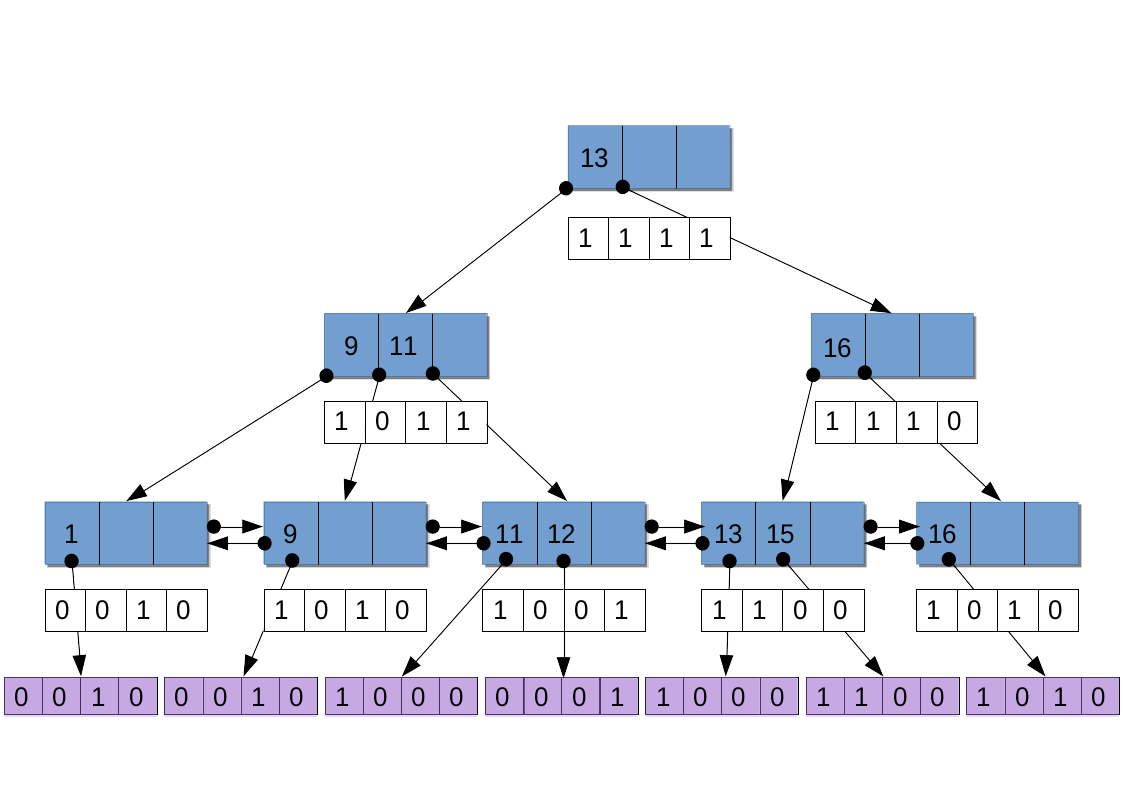
\includegraphics[width=1.0\textwidth]{pictures/bloom-filter-tree.png}\\
  \caption[Aufbau eines BloomFilterTree]{Aufbau eines BloomFilterTree mit Bloom-Filtern als Datensätzen und Vereinigungsfiltern an allen Knoten.}\label{fig:pic6}
\end{figure}
\subsection{Umsetzung}\label{sec:umsetzung}
Die Klasse \texttt{BloomFilterTree} enthält schließlich alle notwendigen Parameter und Operationen zur Organisation der Bloom-Filter. Dazu gehören die B$^+$-Baum-Operationen wie Einfügen und Suchen von Schlüsseln, Traversieren der Blätter, boolesche Abfrage nach Enthaltensein eines Schlüssel im Baum, Zählen der Blätter etc.. Darüber hinaus gibt es viele weitere Operationen: 
\begin{enumerate}
	\item \textit{Management-Operationen} zum Berechnen der Jaccard-Distanzen zu allen Filtern im Baum, naive Version der \textit{k}-nächste-Nachbarn-Suche, Traversieren der Datensätze etc..
	\item Die \textit{zentralen Operationen} des Verfahrens: Einfügen der Bloom-Filter nach Ähnlichkeit und \textit{k}-nächste-Nachbarn-Suche. 
	\item \textit{Mess- und Vergleichsoperationen}, um z.B. Varianten der \textit{k}-nächste-Nachbarn-Suche, Aufbaukosten und Speicherbedarf der Datenstrukturen zu vergleichen. 
\end{enumerate}
Die Header-Datei der Klasse \texttt{BloomFilterTree} ist im Anhang abgedruckt (vgl. Abschnitt \ref{sec:BloomFilterTree.hpp}). In der Klasse \texttt{BloomFilter} wurden alle Parameter und Operationen auf Bloom-Filtern realisiert, die sich im Laufe der Arbeit als wichtig erwiesen. Dazu gehören: 
\begin{enumerate}
	\item \textit{Typische Bloom-Filter-Parameter und -Operationen:} Anzahl der Hashfunktionen, Daten-Array, Setzen von Bitpositionen etc..
	\item \textit{Mathematische und Vergleichsoperationen} wie Berechnung von Teil- und Obermengen, bitweises logisches Und und Oder, Berechnung und Abschätzung von Jaccard-Distanzen.
	\item \textit{Operationen zum Bloom-Filter-Management} wie Einfügen von zufälligen Elementen aus einem Wörterbuch oder zufällige Initialisisierung mit Werten aus $\{0,1\}$.
\end{enumerate}
Die Header-Datei der Klasse \texttt{BloomFilter} findet sich ebenfalls im Anhang (vgl. Abschnitt \ref{sec:BloomFilter.hpp}).
\subsection{Einfügen}\label{sec:einfügen}
Die Einfüge-Operation zählt zu den wichtigsten Funktionen der Indexstruktur. Sie ist entscheidend für die Optimierung von Laufzeit und CPU-Zeit der \textit{k}-nächste-Nachbarn-Suche. Der Algorithmus basiert auf den Teil- und Obermengenbeziehungen zwischen Bloom-Filtern. Er verwendet die Vereinigungsfilter der bereits existierenden Knoten, um die optimale Position für den neu einzufügenden Filter zu finden. Falls der Baum noch leer ist, wird ein neuer Blattknoten erstellt und der Filter als erstes Datenobjekt dort eingefügt. Der neue Knoten wird zur Wurzel des BloomFilterTree. Andernfalls wird ausgehend vom Wurzelknoten rekursiv die optimale Position im Baum gesucht. Dazu werden optimale Teil- und Obermengen-IDs des Filters berechnet. Dem Filter wird die neue Teilmengen-ID zugewiesen und er wird gemäß der B$^+$-Baum-Regeln in den Baum eingefügt. Sind Teilmengen- und Obermengen-IDs unterschiedlich, wird ein zweites Datenobjekt mit der Obermengen-ID erstellt und ebenfalls in den Baum eingefügt. Falls der Baum während des Einfügens eine neue Ebene erhalten hat, wird der Elternknoten des alten Wurzelknoten zur neuen Wurzel. Abbildung \ref{fig:pic7} verdeutlicht den Ablauf:  
\begin{figure}[hpbt]
  \centering
 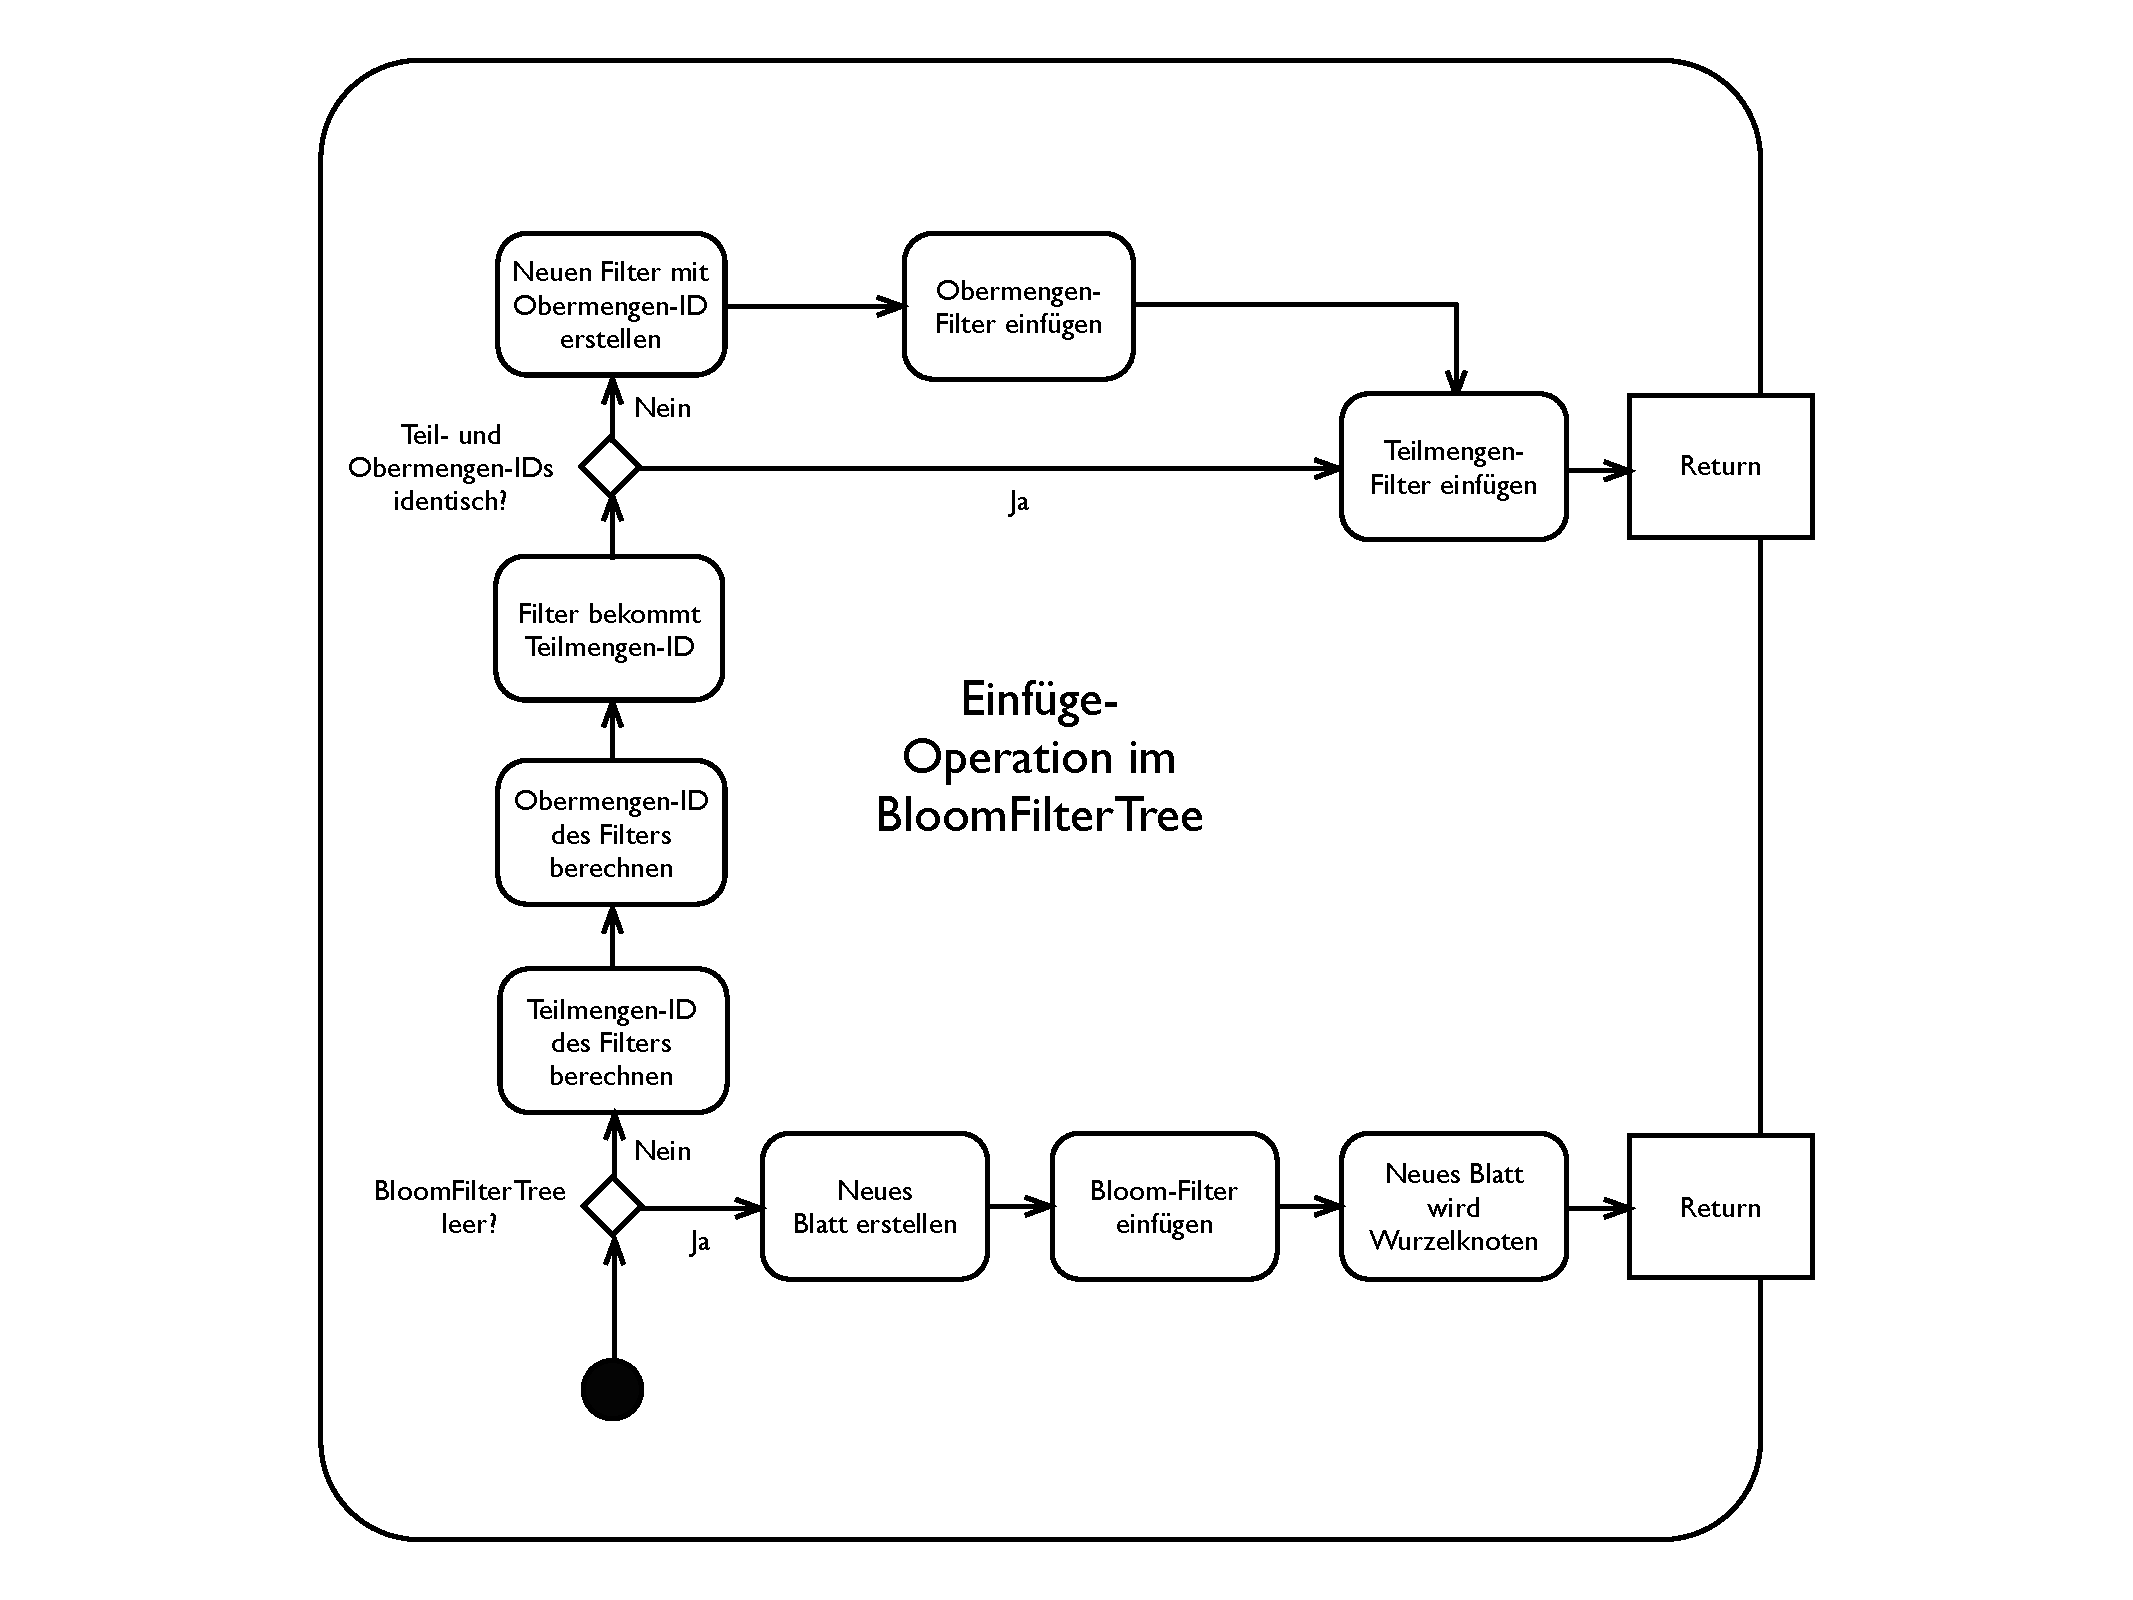
\includegraphics[scale=0.5]{pictures/insert-as-sets.pdf}\\
  \caption[Einfüge-Operation im BloomFilterTree]{Einfüge-Operation im BloomFilterTree.}\label{fig:pic7}
\end{figure}
Die Hauptarbeit des Einfügens findet in den Blattknoten statt, wo die Teilmengen- und Obermengen-IDs der Filter berechnet werden. Zur Berechnung der Teil\-mengen-ID werden folgende Schritte ausgeführt: 
\begin{enumerate}
	\item Einsammeln aller Bloom-Filter-Objekte im Baum, von denen der einzufügende Filter eine Teilmenge ist.
	\item Sortieren der gesammelten Filter nach Jaccard-Distanz in aufsteigender Reihenfolge.
	\item Einsammeln aller freien IDs im Baum zwischen der kleinsten und größten ID. 
	\item Sortieren der freien IDs in aufsteigender Reihenfolge.
	\item Falls der Filter von keinem Objekt im Baum eine Teilmenge ist, wird die kleinste freie ID zurückgegeben. 
	\item Andernfalls wird die optimale Teilmengen-ID bestimmt. Dazu werden zu allen in Schritt 2 gesammelten Filtern jeweils die nächstgrößere und nächstkleinere freie ID bestimmt. Diese "`guten"' IDs werden in einem Vektor gesammelt. 
	\item Die "`guten"' IDs werden nach Distanz zu einem Teilmengen-Filter des Anfragefilters sortiert. 
	\item Die ID mit der kleinsten Distanz zu einem Filter, von der der neu einzufügende Filter eine Teilmenge ist, wird als Ergebnis zurückgegeben. 
\end{enumerate}
Die Funktion \texttt{computeSubsetId()} der Klasse \texttt{BloomFilterLeaf} ist beispielhaft im Anhang abgedruckt (vgl. Abschnitt \ref{sec:computeSubsetId()}). Die Berechnung der optimalen Obermengen-ID geschieht analog dazu in der Funktion \texttt{computeSupersetId()}, nur dass dazu die Obermengen des neuen Filters betrachtet werden. 
\subsection{\textit{k}-nächste-Nachbarn-Suche}\label{sec:knn}
Das eben beschriebene Verfahren zum Einfügen von Objekten ist wesentlich aufwändiger als normalerweise beim B$^+$-Baum. Die Berechnung der optimalen Teil- und Obermengen-IDs für einen neuen Filter dient dazu, Filter mit bestehenden Teil- und Obermengenbeziehungen nahe beieinander im Baum abzuspeichern. Die \textit{k}-nächste-Nachbarn-Suche musste natürlich darauf abgestimmt werden. Sie vergleicht nicht wie in der naiven Implementierung \textit{k}-mal die Distanzen aller Bloom-Filter im Baum zum Anfragefilter und gibt die Filter mit den \textit{k} kleinsten Distanzen zurück. Stattdessen werden die Vereinigungsfilter der Baumknoten danach untersucht, ob sie zum Anfragefilter in Teil- oder Obermengenbeziehung stehen. Ziel ist es, bei einer Anfrage nur den besten Zweig im Baum zu verfolgen.

Wie im vorigen Abschnitt dargestellt, werden die Filter beim Einfügen nach Teil- und Obermengenbeziehungen angeordnet. Der Vereinigungsfilter jedes Baumknotens enthält die Vereinigungsmenge aller Filter in seinem Teilbaum. Damit lässt sich die \textit{k}-nächste-Nachbarn-Suche deutlich verkürzen. 

Da die \textit{k}-nächste-Nachbarn-Suche teurer und aufwändiger ist als eine Punktanfrage nach einem Objekt, wurden dafür zwei verschiedene Operationen implementiert. Die Punktanfrage geschieht in folgenden Schritten: 
\begin{enumerate}
	\item Falls der Baum leer ist, wird der Zeiger auf den Anfragefilter selbst zurückgegeben. 
	\item Andernfalls wird geprüft, ob der Wurzelknoten Teil- oder Obermenge des Anfragefilters ist. 
	\item Ist das nicht der Fall, wird eine normale nächste-Nachbarn-Suche auf dem Baum ausgeführt. 
	\item Andernfalls wird rekursiv beim Wurzelknoten beginnend geprüft, welche Vereinigungsfilter der Kindknoten Teil- oder Obermengen des Anfragefilters sind. 
	\item Gibt es mehrere davon, wird der Kindknoten mit der kleinsten Jaccard-Distanz des Vereinigungsfilters zum Anfragefilter bestimmt. Nur dieser Pfad wird weiter verfolgt.
	\item Gibt es keine Teil Teil- oder Obermengenbeziehungen zu den Vereinigungsfiltern der Kindknoten, wird eine nächste-Nachbarn-Suche auf dem restlichen Teilbaum durchgeführt. 
	\item Ist die Anfrage auf der Blattebene angekommen, wird der Filter mit der kleinsten Distanz im Blatt bestimmt und ein Zeiger darauf zurückgegeben.  
\end{enumerate}
Auch wenn ab einem bestimmten Punkt keine Teil- oder Obermengenbeziehungen mehr zwischen Anfragefilter und den Vereinigungsfiltern der Kindnoten des aktuellen Knoten bestehen, wird die Anfrage deutlich abgekürzt. Dann muss nur noch eine nächste-Nachbarn-Suche auf einem Teilbaum durchgeführt werden, nicht auf der gesamten Indexstruktur. 

Hier findet offensichtlich die hauptsächliche Arbeit in den inneren Knoten des BloomFilterTree statt, den so genannten Index- oder Directoryknoten. Bei der \textit{k}-nächste-Nachbarn-Suche findet hingegen wie zuvor ein großer Teil der Sortierarbeit auf Blattebene statt. Abbildung \ref{fig:pic8} zeigt den Ablauf im BloomFilterTree: 
\begin{figure}[hpbt]
  \centering
  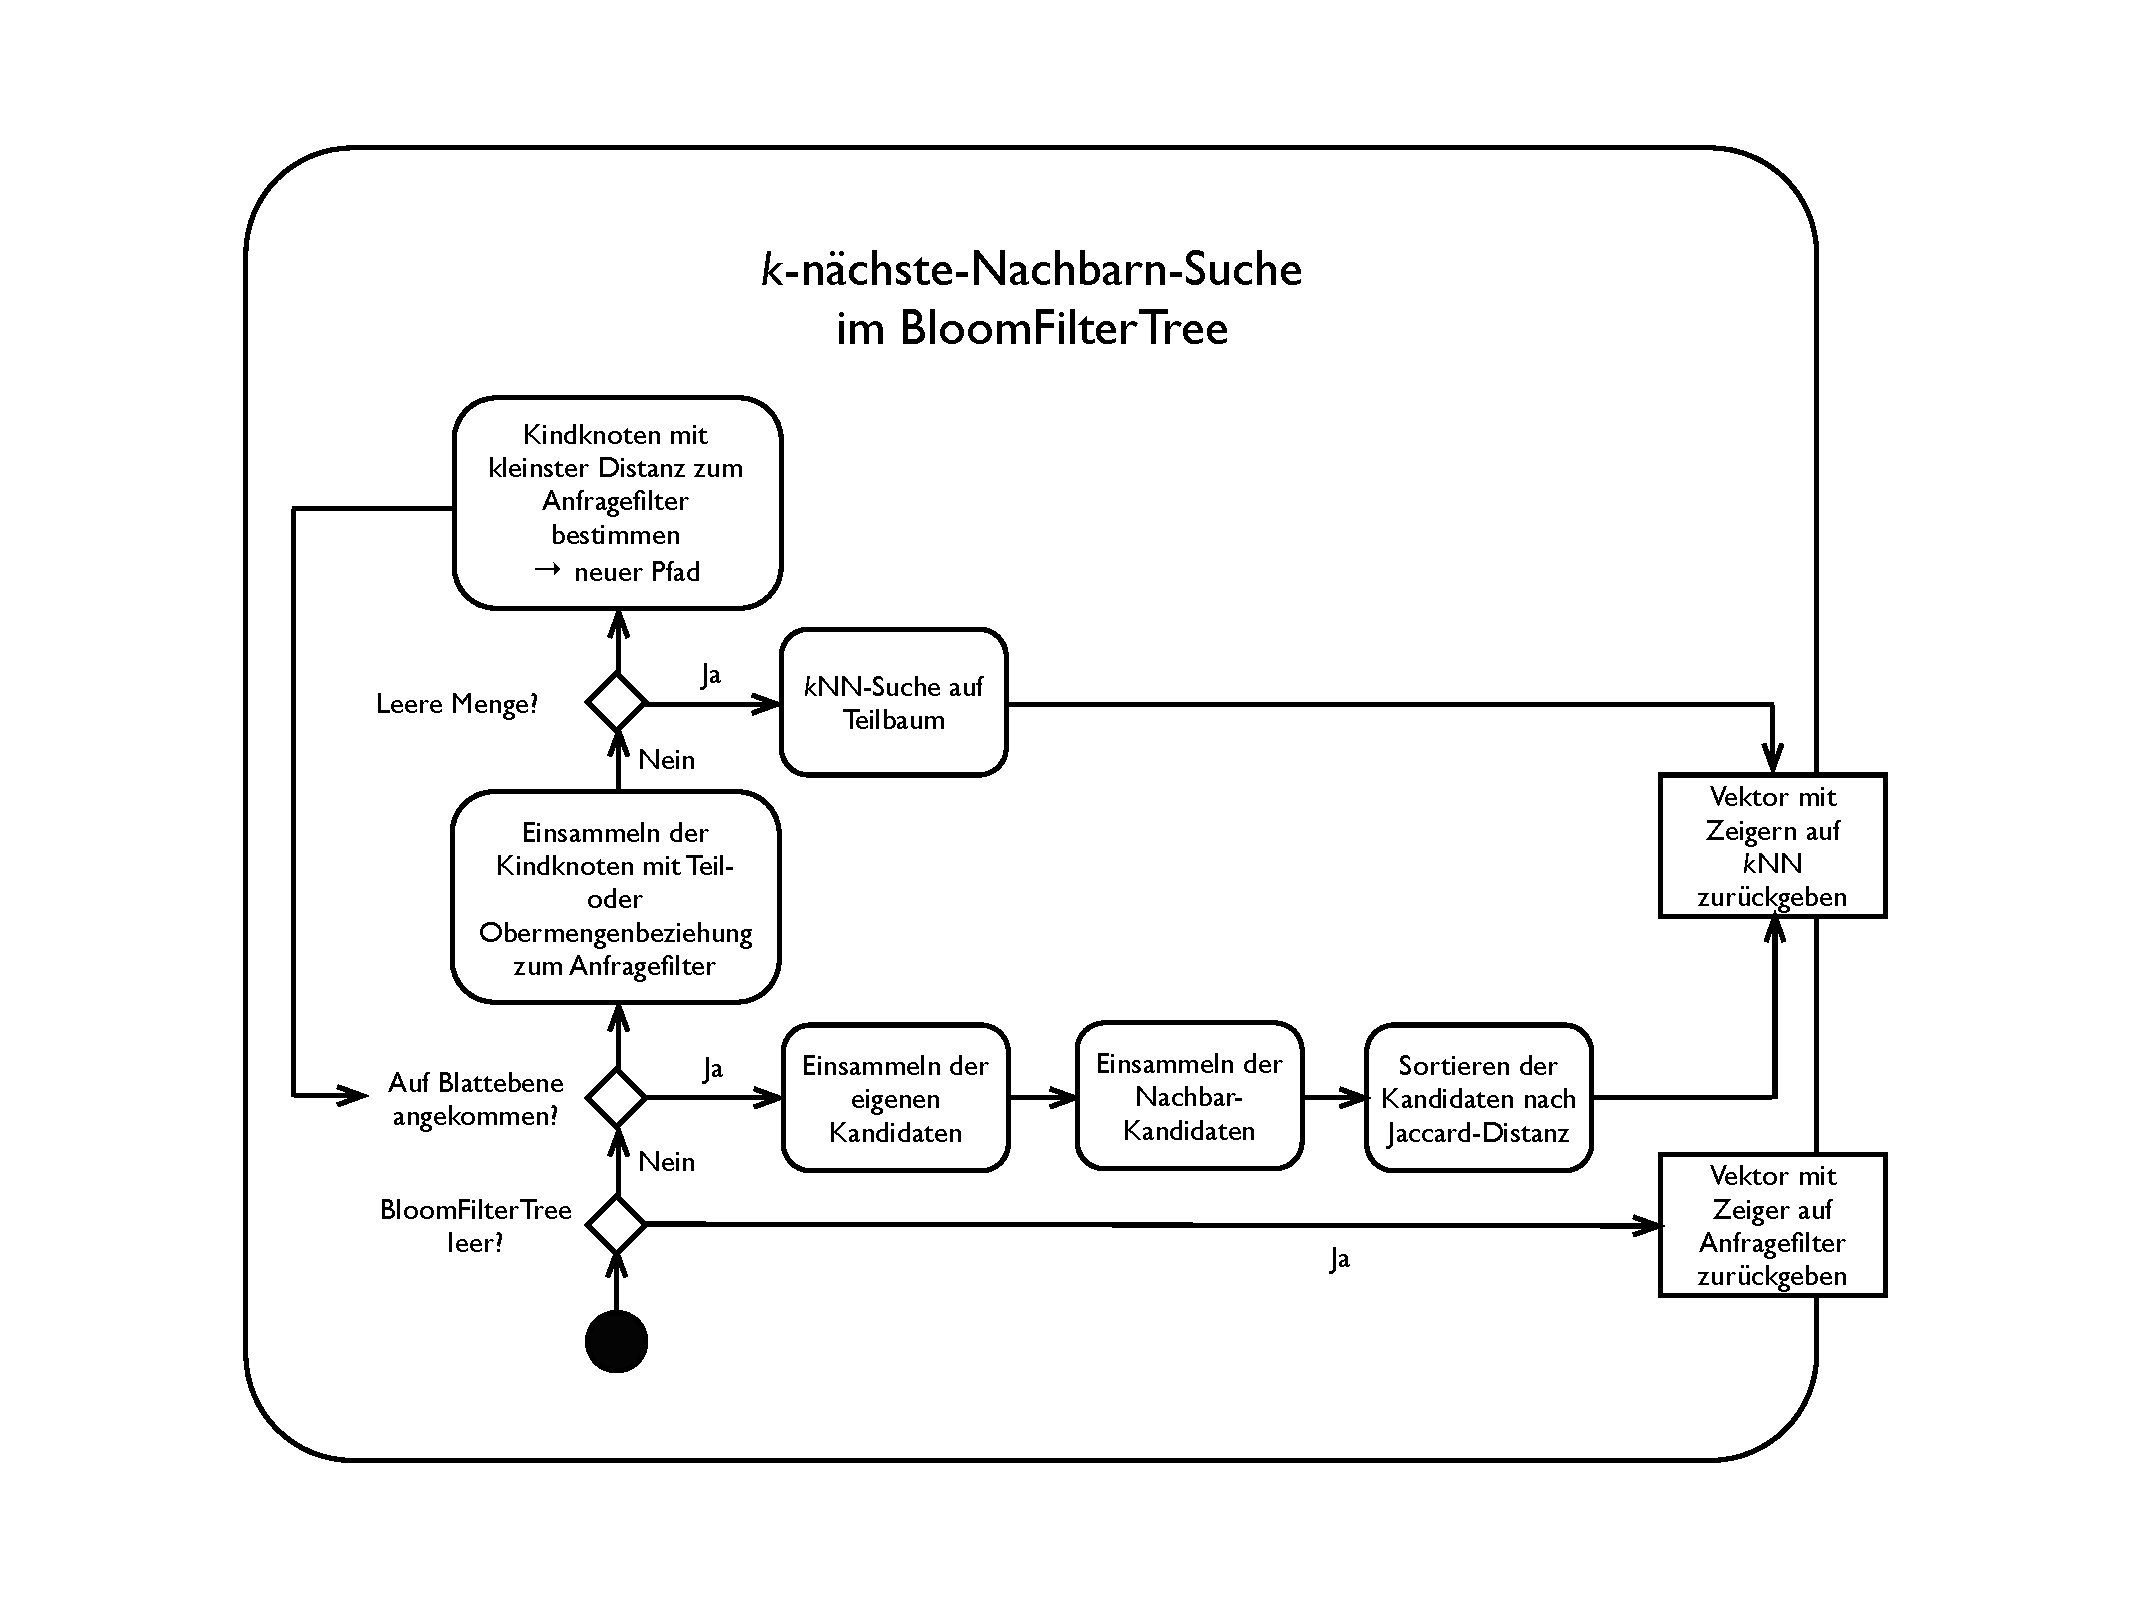
\includegraphics[scale=0.5]{pictures/knn.pdf}\\
  \caption[\textit{k}-nächste-Nachbarn-Suche im BloomFilterTree]{\textit{k}-nächste-Nachbarn-Suche im BloomFilterTree.}\label{fig:pic8}
\end{figure}
Der Quellcode der Funktion \mbox{\texttt{simQueryVec()}} der Klasse \texttt{BloomFilterTree} ist beispielhaft im Anhang abgedruckt (vgl. \ref{sec:simQueryVec()}). Wie die Evaluation in Kapitel \ref{ch:evaluation} zeigt, lassen sich mit den vorgestellten Methoden Laufzeit und CPU-Zeit der \textit{k}-nächste-Nachbarn-Suche deutlich reduzieren. 

Es sei angemerkt, dass die B$^+$-Baum-spezifische Bereichssuche bei allen vorgestellten Funktionen von Nutzen ist. Die Einfüge-Operation wird z.B. dadurch erleichtert, dass zum Einsammeln aller freien IDs nur einmal die Blattebene traversiert werden muss. Andere Baumstrukturen benötigen dazu in der Regel eine deutlich komplexere Breiten- oder Tiefensuche. Bei der \textit{k}-nächste-Nachbarn-Suche in einem Teilbaum muss ebenfalls nur der Teilbereich zwischen einem Start- und Endwert traversiert werden. Das liegt daran, dass die Blätter eine doppelt verkettete Liste bilden und die Indexstruktur die Suchbaumeigenschaft auf den Primärschlüsseln, d.h. den Bloom-Filter-IDs, erfüllt.  
\section{Alternative Ansätze}\label{sec:alternativen}
Zum Abschluss des Kapitels werden zwei Ansätze vorgestellt, die alternativ zum BloomFilterTree bzw. zur Organisation nach Teil- und Obermengenbeziehungen verfolgt wurden. Letztlich erwies sich jedoch die Kombination aus Baumstruktur und Mengenbeziehungen am erfolgreichsten. 
\subsection{Einfügen gemäß Jaccard-Distanzen}\label{sec:ähnlichkeit}
Anfangs wurde der Ansatz verfolgt, die Bloom-Filter wie bei Sakuma und Sato an Hand ihrer Distanzen im Baum zu organisieren (vgl. Abschnitt \ref{sec:bloom-index}). Dabei stellte sich heraus, dass das dort verwendete Distanzmaß transitiv ist im Sinne von Abschnitt \ref{sec:distanzmasse}. Das trifft auf die Jaccard-Distanz nicht zu. Die Suche nach Alternativen ergab die Kombination aus Vereinigungsfilter und Transitivität der Teil- und Obermengenbeziehungen, die letztlich umgesetzt wurde. 
\subsection{Doppelt verkettete Liste}\label{sec:verkettete-liste}
Eine andere Idee war die Gruppierung der Filter nach Gleichheit von Teilsegmenten. Als Datenstruktur sollte eine doppelt verkettete Liste dienen mit derselben Anzahl an Listenknoten wie Positionen im Bloom-Filter. Die einzufügenden Bloom-Filter wurden in Segmente unterteilt. Ein Segment entsprach dabei einem Element im Daten-Array. Ein neuer Filter wurde wie folgt in die Datenstruktur eingefügt:  
\begin{enumerate}
	\item Jeder Listenknoten hat eine 0- und eine 1-Bit-Liste. Darin sind Zeiger auf die bereits eingefügten Filter gespeichert, die an derselben Bitposition eine 0 bzw. eine 1 enthalten. 
	\item Wird ein neues Objekt in die Liste eingefügt, wird an jedem Listenknoten die entsprechende Liste aktualisiert, je nachdem, ob der einzufügende Filter an der Position 0 oder 1 enthält. 
\end{enumerate}
Das Ziel war, bei der \textit{k}-nächsten-Nachbarn-Suche die 0- bzw. 1-Bit-Listen der Listenknoten mit gleichem Segmentinhalt abzuprüfen. Alle darin enthaltenen Zeiger wurden in einem Vektor gesammelt, der nach Häufigkeit der Zeiger sortiert wurde. Es bestand die Hoffnung, dass sich die am häufigsten vorkommenden Zeigern und die nächsten Nachbarn des Anfragefilters proportional zueinander verhielten.
 
Eine solche Datenstruktur ist in Implementierung und Pflege weit weniger aufwändig als eine Baumstruktur. Es zeigte sich jedoch, dass damit nicht die gewünschten Ergebnisse erzielt werden konnten, da bei der \textit{k}-nächste-Nachbarn-Suche zu viele Ergebnisse mit gleich vielen Zeigern gefunden wurden. Die Suche scheiterte somit an mangelnder Ergebnisqualität und die doppelt verkettete Liste wurde als Datenstruktur verworfen. 
    \chapter{Evaluation}\label{ch:evaluation}
Das folgende Kapitel dient dem Vergleich zwischen der entwickelten Datenstruktur und der bisherigen Organisation der Bloom-Filter in AMBIENCE. Abschnitt \ref{sec:datensatz} beschreibt zunächst den für die Evaluation verwendeten Datensatz. Dieser stammt nicht aus AMBIENCE, sondern die Bloom-Filter wurden wie in Abschnitt \ref{sec:umsetzung} beschrieben selbst implementiert. Der Versuchsaufbau, d.h. welche Aspekte der Indexstruktur untersucht und verglichen wurden, findet sich in Abschnitt \ref{sec:versuchsaufbau}. Die erzielten Ergebnisse werden in Abschnitt \ref{sec:ergebnisse} vorgestellt und in Abschnitt \ref{sec:interpretation} ausgewertet.
\section{Datensatz}\label{sec:datensatz}
Obgleich nicht mit echten AMBIENCE-Daten gearbeitet wurde, wurde ein möglichst realistisches Szenario erstellt mit folgenden Parametern:
\begin{center}
\begin{table}[htbp]
{\small
\begin{center}
\begin{tabular}[center]{lcc}
\toprule
\textbf{Filtergröße} & 256 Bit & 512 Bit\\
\midrule
\textbf{Anzahl Bloom-Filter (m)} & 100 & 100\\
\midrule
\textbf{Anzahl eingefügte Objekte (n)} & 50 & 50\\
\midrule
\textbf{Anzahl Hashfunktionen (d)} & 4 & 8\\
\bottomrule
\end{tabular}
\end{center}
} % end of tiny
\caption[Datensatz für den Versuchsaufbau]{Datensatz für den Versuchsaufbau.\label{tab:Datensatz}}
\end{table}
\end{center}
Als Wörterbuch wurde die Unix-Datei \texttt{words} verwendet, aus der jeweils 50 zufällige Einträge in die Bloom-Filter eingefügt wurden. Wie in Abschnitt \ref{sec:hashfunktionen} erläutert, wurden zum Einfügen Murmur-Hashfunktionen verwendet. Die Anzahl der zu verwendenden Hashfunktionen lässt sich berechnen als 
\[d = \Ceil[\Bigg]{\frac{m}{n} * ln(2)}.\]
\noindent
Der \textit{i+1}-te Hashwert wurde dabei jeweils aus dem \textit{i}-ten Hashwert berechnet wie in Abschnitt \ref{sec:bloom-implementierung} beschrieben. Den Bloom-Filtern wurden zunächst zufällige IDs zugewiesen. Sie wurden jeweils in einen BloomFilterTree mit 256 bzw. 512 Bit Filtergröße und in einen Bloom-Filter-Vektor\footnote{Objekte vom Typ \texttt{std::vector<BloomFilter>}.} eingefügt, der die unsortierte Liste repräsentiert.
\newpage
\section{Versuchsaufbau}\label{sec:versuchsaufbau}
Der Versuchsaufbau vergleicht die Indexstruktur BloomFilterTree mit einer unsortierten Liste von Bloom-Filtern, die der bisherigen Implementierung in AMBIENCE entspricht. Für beide Filtergrößen wurden fünf Experimente durchgeführt:  
\begin{enumerate}
	\item Ergebnisqualität
	\item CPU-Zeit 
	\item Speicherbedarf 
	\item Komplexität 
	\item Aufbaukosten 
\end{enumerate}
\paragraph*{Ergebnisqualität}
Zur Ermittlung der Ergebnisqualität wurde eine nächste-Nachbarn-Suche und eine 3-nächste-Nachbarn-Suche auf dem BloomFilterTree durchgeführt. Die erzielten Ergebnisse wurden mit den Sollwerten einer regulären \textit{k}-nächste-Nachbarn-Suche verglichen. 
\paragraph*{CPU-Zeit}
Zur Messung der CPU-Zeit wurde die C++-Bibliothek \texttt{chrono} verwendet. Es wurden jeweils die Ausführungszeiten der Funktionen \texttt{simQuery()} und \texttt{simQueryVec()} für einen bzw. 3 nächste Nachbarn (vgl. Abschnitt \ref{sec:knn}) ermittelt und mit den Ausführungszeiten einer regulären \textit{k}-nächste-Nachbarn-Suche verglichen.
\paragraph*{Speicherbedarf} 
Da der BloomFilterTree nur Zeiger auf Bloom-Filter-Objekte enthält und nicht die Datenstrukturen selbst, ist sein Speicherbedarf sehr gering. %TODO Angabe 
Zur Ermittlung des Speicherbedarfs wurde daher von den tatsächlich allokierten Instanzen der Klasse \texttt{BloomFilter} ausgegangen. Das sind bei einer unsortierten Liste alle eingefügten Bloom-Filter, beim BloomFilterTree zusätzlich die Vereinigungsfilter aller Knoten. Diese Speicherbedarfe wurden für BloomFilterTree und unsortierte Liste ermittelt und gegenüber gestellt. 
\paragraph*{Komplexität}
Zur Ermittlung der Komplexität der unterschiedlichen Suchalgorithmen wurde die Anzahl Vergleiche, die zur Anfragebeantwortung notwendig sind, als Maß vorausgesetzt. Diese wurden für BloomFilterTree und unsortierte Liste ermittelt und verglichen. Für den BloomFilterTree wurden dazu Varianten der Funktionen \texttt{simQuery()} und \texttt{simQueryVec()} implementiert, die die Anzahl an durchgeführten Vergleichen exakt mitprotokollieren.   
\paragraph*{Aufbaukosten}
In diesem Experiment wurden die Kosten für den Aufbau der Daten- bzw. Indexstruktur. Als Maß hierfür wurde die Zeitkomplexität des Einfügens aller Elemente bestimmt. Diese liegt für Objekte vom Typ /texttt{std::vector} mit \textit{n} Elementen durchschnittlich in $O(1)$ für die verwendete Funktion \texttt{std::vector::push\_back()}\footnote{Vgl. \url{http://www.cplusplus.com/reference/vector/vector/push_back/.}}. 

\noindent
Beim BloomFilterTree setzt sich die Komplexität der Einfüge-Operation aus der Berechnung der optimalen Teilmengen- und Obermengen-IDs und dem tatsächlichen Einfügen des Elements zusammen. Wie in Abschnitt \ref{sec:einfügen} dargestellt, ist die Berechnung der Teilmengen-IDs relativ rechenintensiv und deutlich teurer als das kanonische Einfügen im B$^+$-Baum. Die teuersten Operationen sind hierbei das Sortieren der freien und "`guten"' IDs. Die Kosten für den Aufbau der Indexstruktur liegen damit insgesamt in $O(n\ast log(n))$ für einen BloomFilterTree mit \textit{n} Elementen. 
\section{Ergebnisse}\label{sec:ergebnisse}
Im Folgenden werden die Ergebnisse der fünf Experimente mit den eingangs beschriebenen Parametern vorgestellt. 
\paragraph*{Ergebnisqualität}
Abbildungen \ref{fig:pic8} und \ref{fig:pic9} stellen die Ergebnisqualität der nächste-Nachbarn-Suche dar. Die Sollwerte sind darin grün, die Messwerte blau markiert. Stimmt der Messwert mit dem Sollwert überein, ist nur die blaue Markierung vorhanden. Der quadratische Fehler von Messwert gegenüber Sollwert ist in Rot angegeben. 
\begin{figure}[hpbt]
	\centering
 	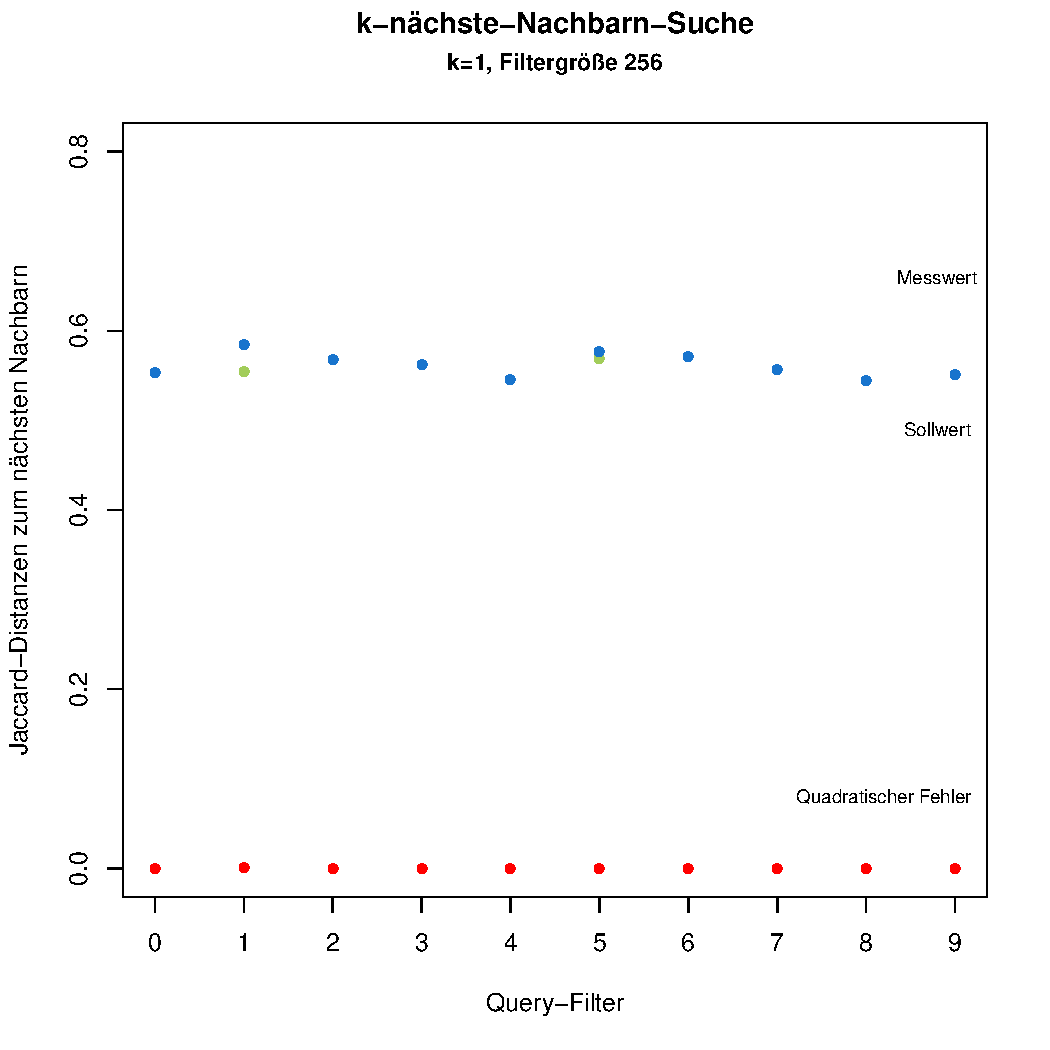
\includegraphics[scale=0.7]{pictures/nn_256.pdf}\\
  	\caption[Ergebnisqualität der nächste-Nachbarn-Suche für 256 Bit-Bloom-Filter]{Ergebnisqualität der nächste-Nachbarn-Suche für 256 Bit-Bloom-Filter.}\label{fig:pic7}
 	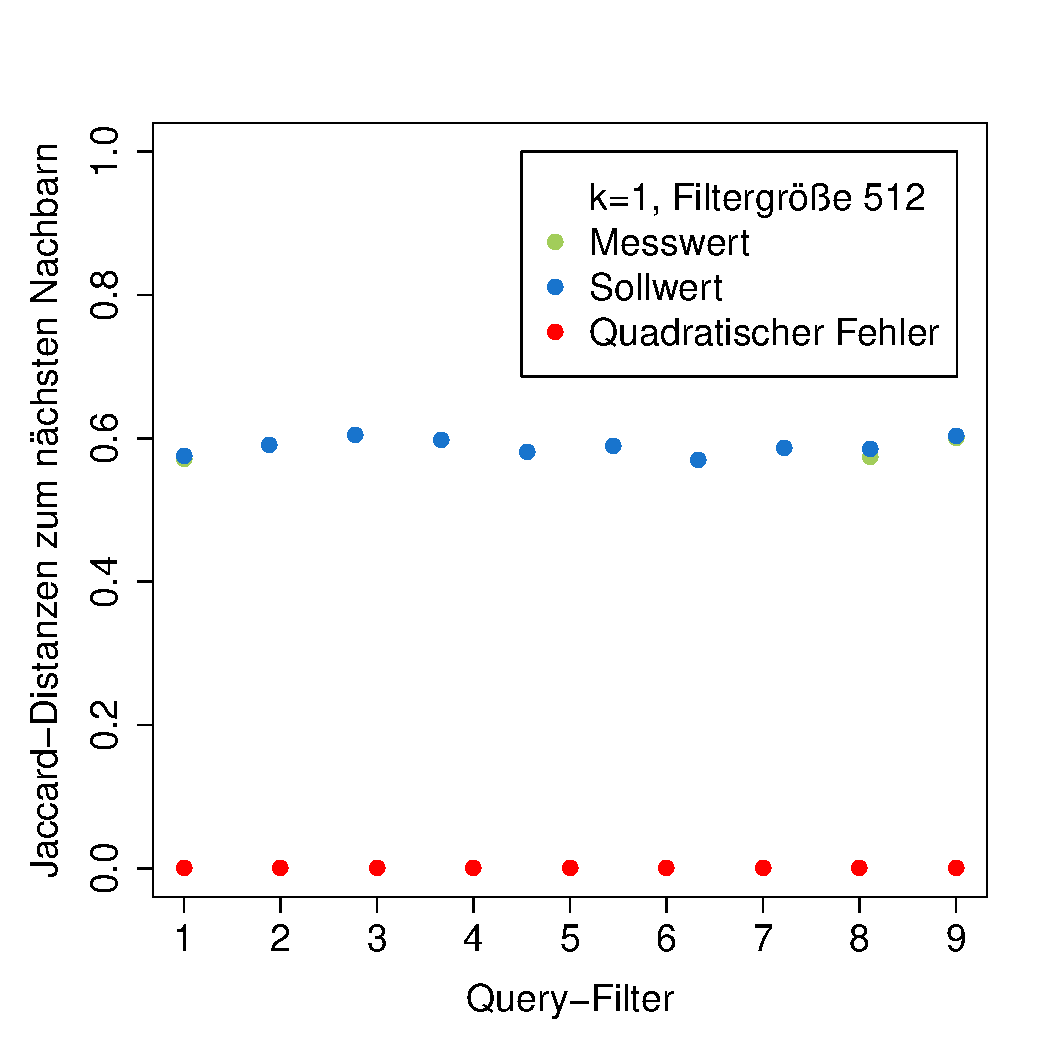
\includegraphics[scale=0.7]{pictures/nn_512.pdf}\\
  	\caption[Ergebnisqualität der nächste-Nachbarn-Suche für 256 Bit-Bloom-Filter]{Ergebnisqualität der nächste-Nachbarn-Suche für 512 Bit-Bloom-Filter.}\label{fig:pic8}
\end{figure}
Abbildungen \ref{fig:pic9} -- \ref{fig:pic12} stellen die Ergebnisqualität der 3-nächste-Nachbarn-Suche dar. Die Sollwerte sind darin in drei Grünstufen markiert, die Messwerte sind in drei Blaustufen markiert. Der mittlere quadratische Fehler der Messwerte gegenüber den Sollwerten ist in Rot angegeben.
\begin{figure}
	\centering
	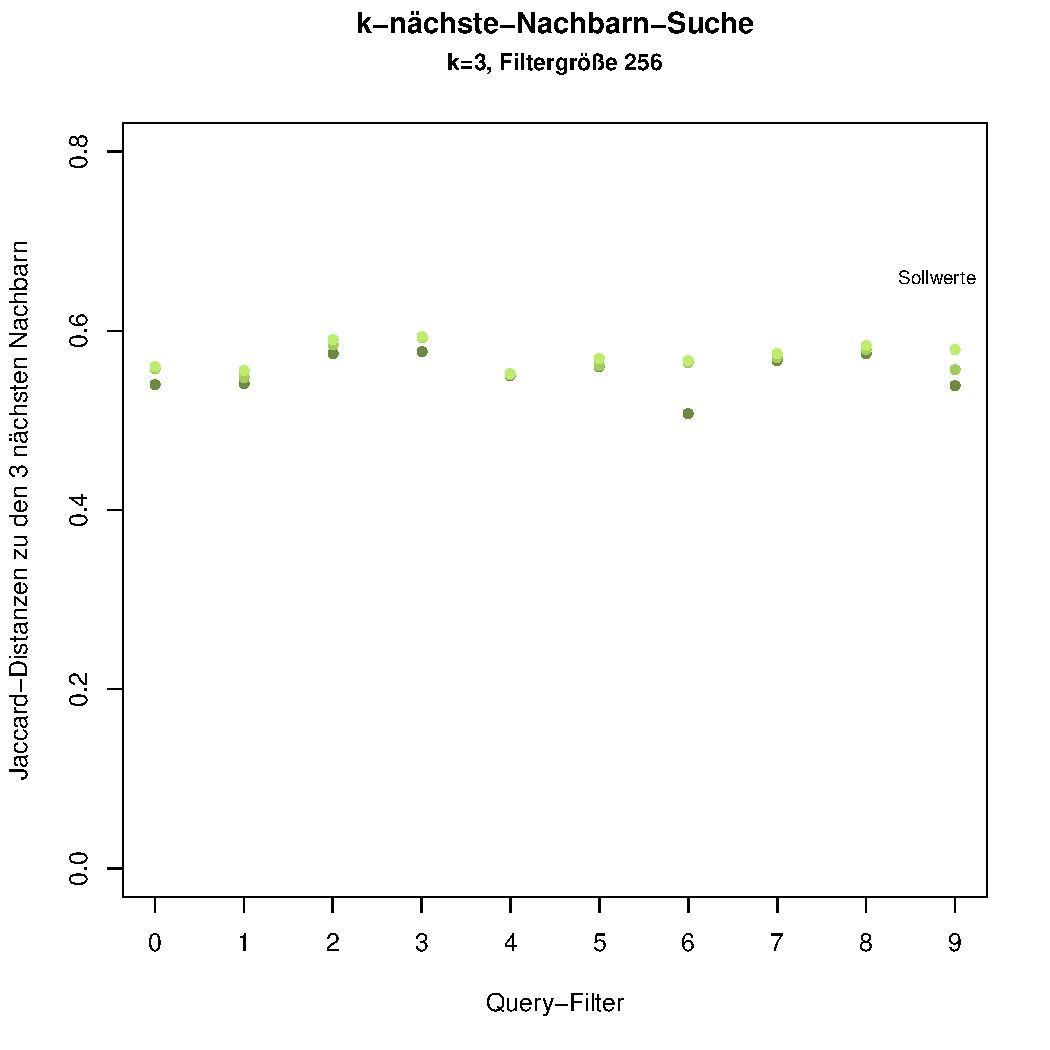
\includegraphics[scale=0.7]{pictures/nn3_256-1.pdf}\\
	\caption[Sollwerte der 3-nächste-Nachbarn-Suche für 256 Bit-Bloom-Filter]{Sollwerte der 3-nächste-Nachbarn-Suche für 256 Bit-Bloom-Filter.}\label{fig:pic9}
	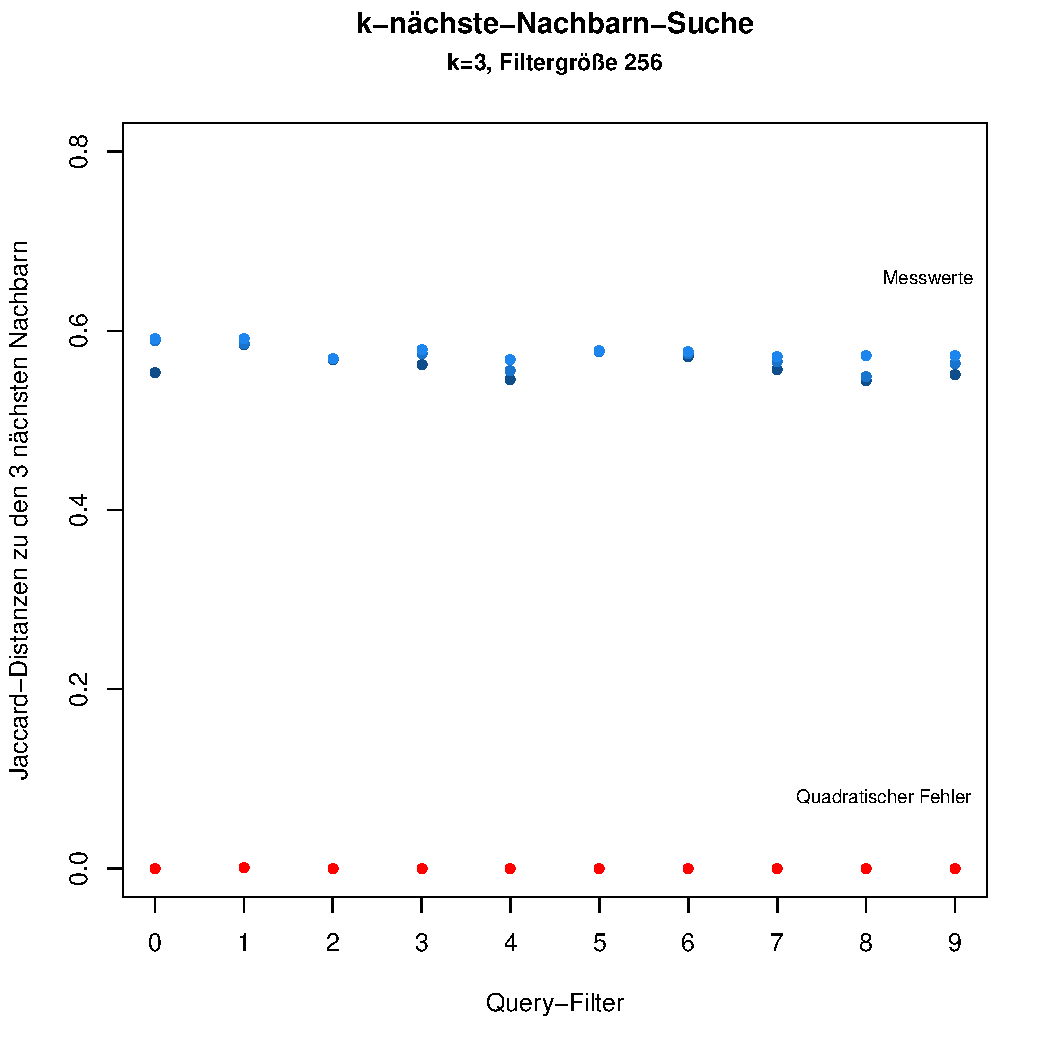
\includegraphics[scale=0.7]{pictures/nn3_256-2.pdf}\\
	\caption[Messwerte der 3-nächste-Nachbarn-Suche für 512 Bit-Bloom-Filter]{Messwerte der 3-nächste-Nachbarn-Suche für 512 Bit-Bloom-Filter.}\label{fig:pic10}
\end{figure}
\begin{figure}[hptb]
	\centering
	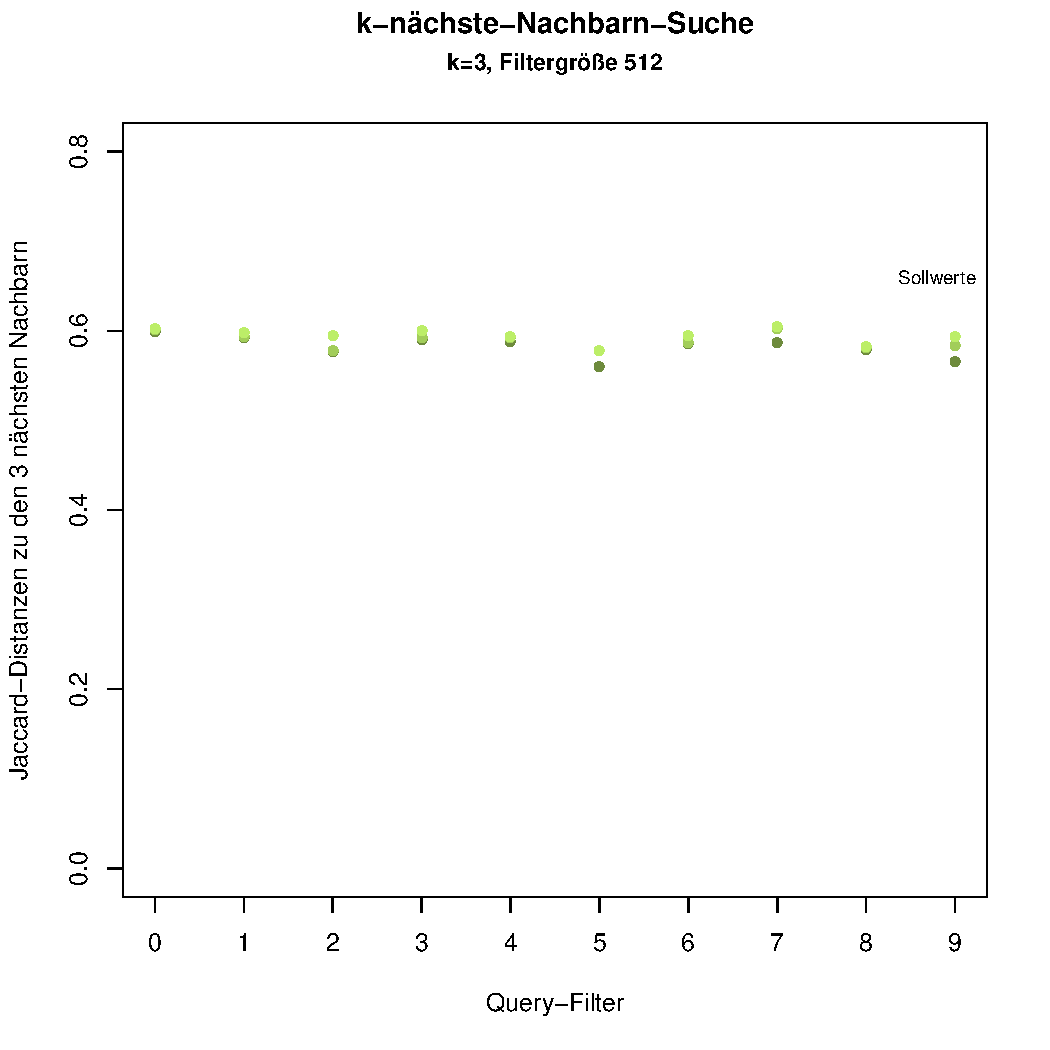
\includegraphics[scale=0.7]{pictures/nn3_512-1.pdf}\\
	\caption[Sollwerte der 3-nächste-Nachbarn-Suche für 512 Bit-Bloom-Filter]{Sollwerte der 3-nächste-Nachbarn-Suche für 512 Bit-Bloom-Filter.}\label{fig:pic11}
	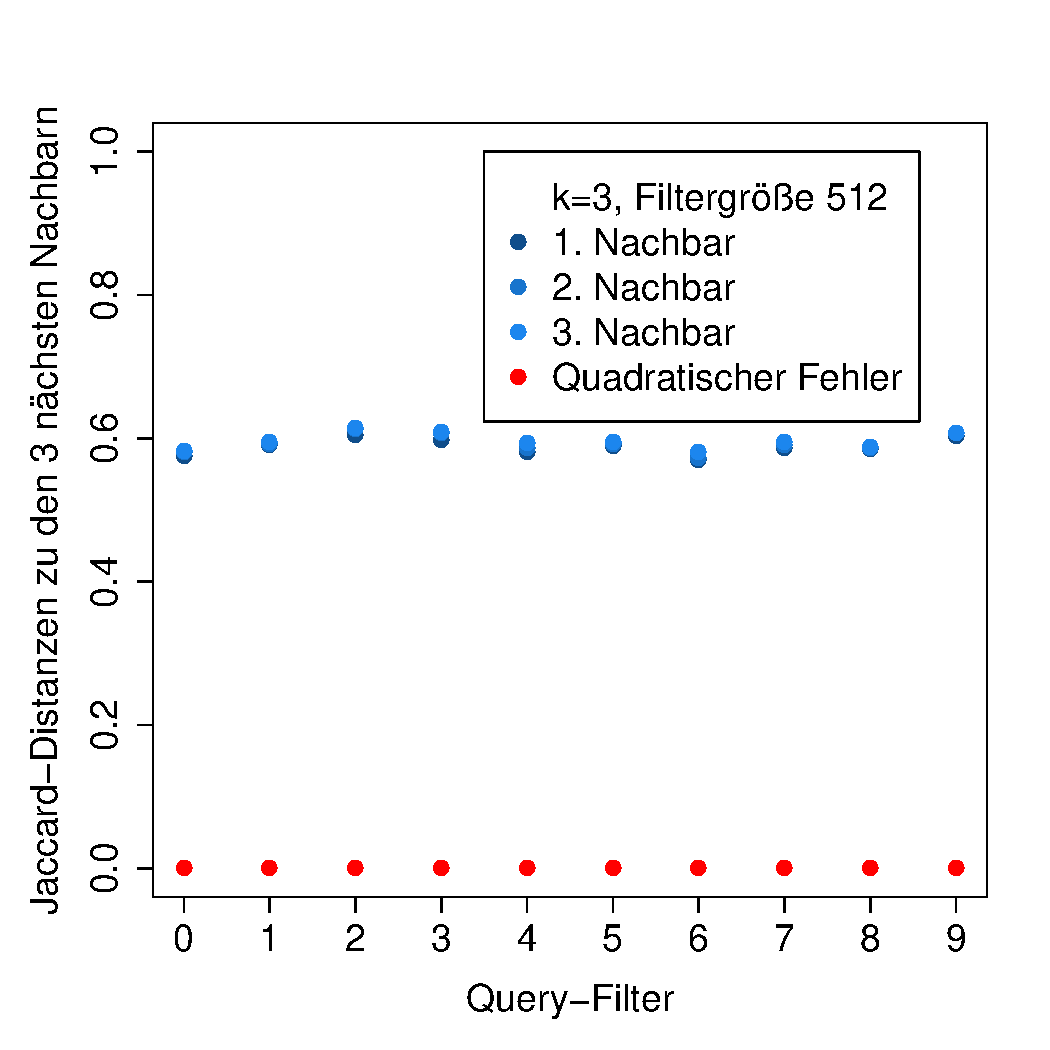
\includegraphics[scale=0.7]{pictures/nn3_512-2.pdf}\\
	\caption[Messwerte der 3-nächste-Nachbarn-Suche für 512 Bit-Bloom-Filter]{Messwerte der 3-nächste-Nachbarn-Suche für 512 Bit-Bloom-Filter.}\label{fig:pic12}
\end{figure}
\paragraph*{CPU-Zeit}
Abbildungen \ref{fig:pic13} und \ref{fig:pic14} stellen die CPU-Zeit zur Ausführung der nächste-Nachbarn-Suche dar. Die Ergebnisse für den BloomFilterTree sind darin blau, die Ergebnisse für die unsortierte Liste grün markiert.  
\begin{figure}[hptb]
	\centering
	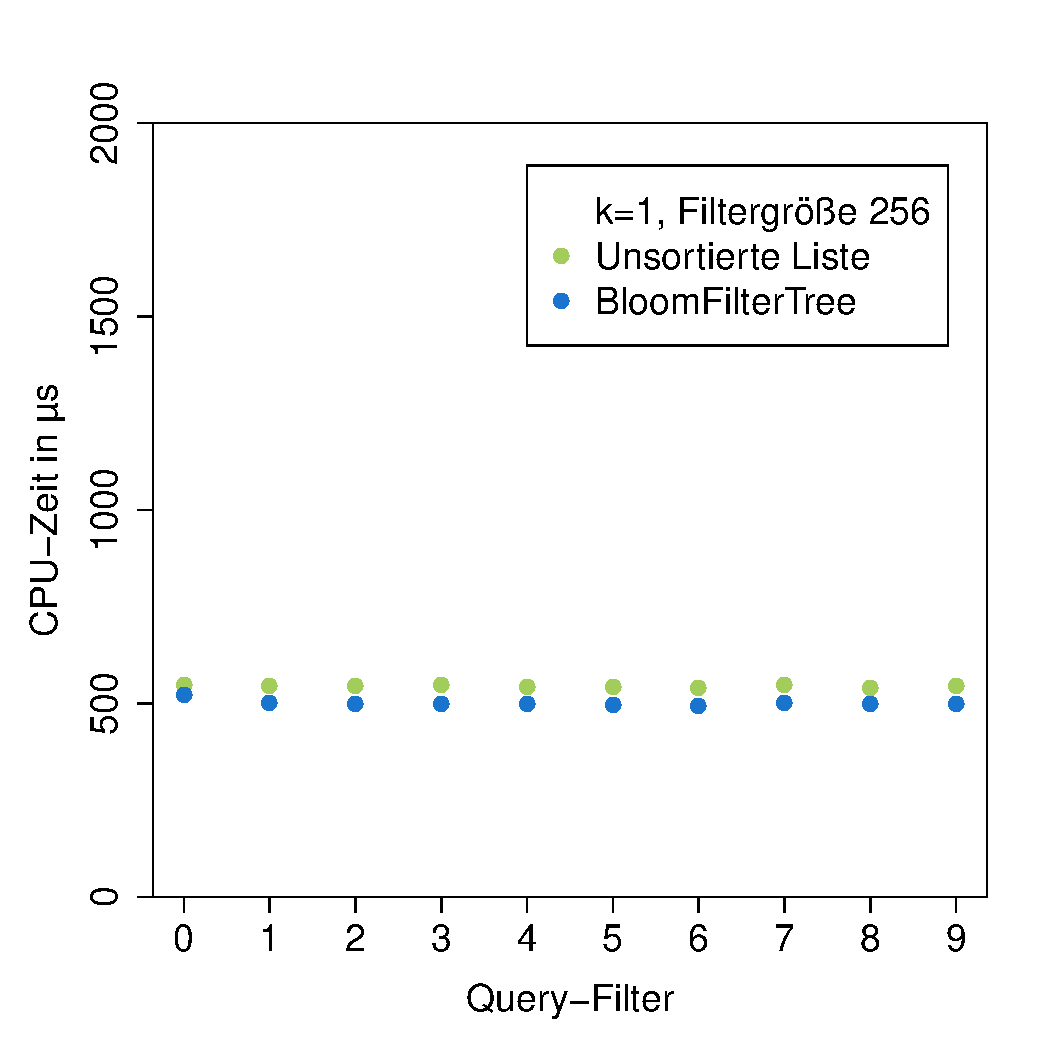
\includegraphics[scale=0.7]{pictures/cputime_nn_256.pdf}\\
	\caption[CPU-Zeit für nächste-Nachbarn-Suche mit 256 Bit-Bloom-Filtern]{CPU-Zeit für \textit{k}-nächste-Nachbarn-Suche mit 256 Bit-Bloom-Filtern.}\label{fig:pic13}
	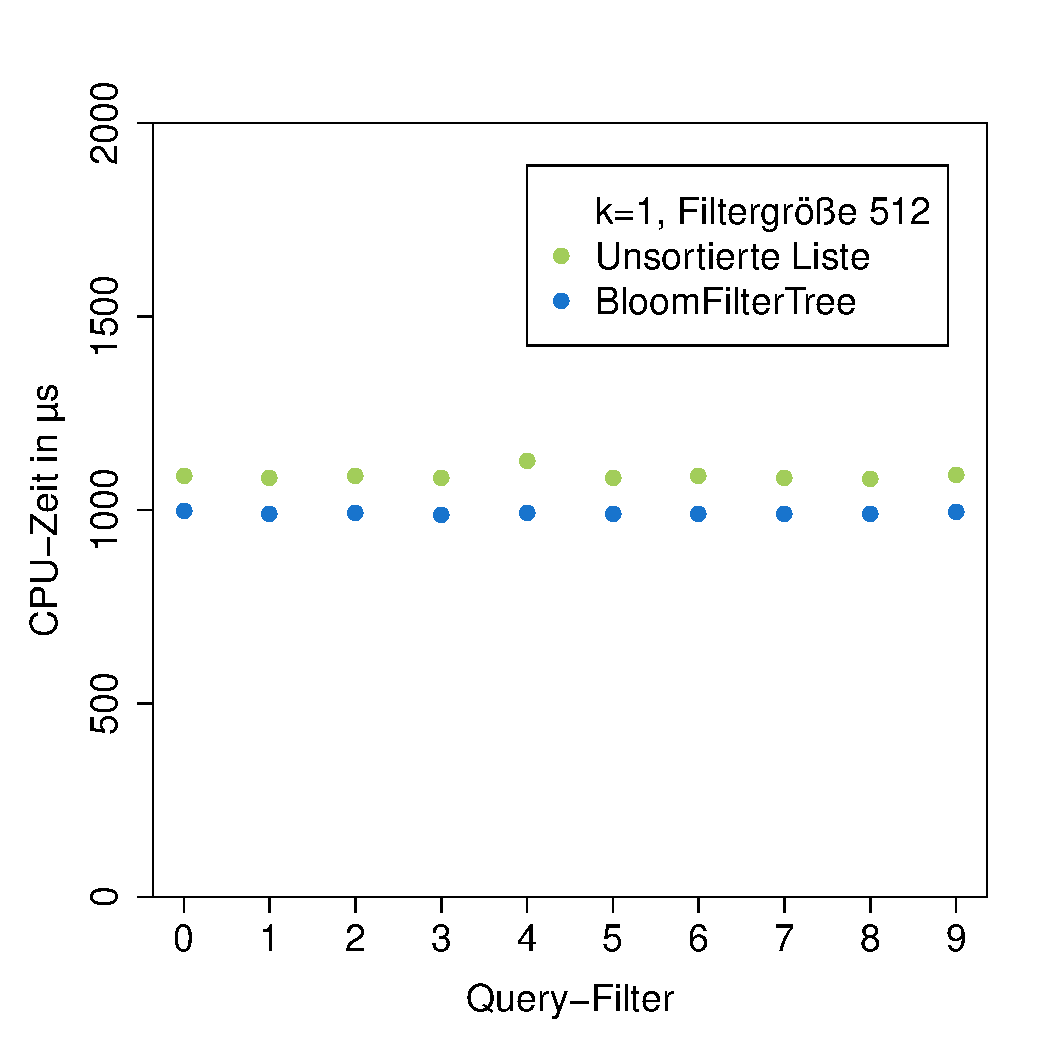
\includegraphics[scale=0.7]{pictures/cputime_nn_512.pdf}\\
	\caption[CPU-Zeit für nächste-Nachbarn-Suche mit 512 Bit-Bloom-Filtern]{CPU-Zeit für \textit{k}-nächste-Nachbarn-Suche mit 512 Bit-Bloom-Filtern.}\label{fig:pic14}
\end{figure}
Abbildungen \ref{fig:pic15} und \ref{fig:pic16} stellen die CPU-Zeit zur Ausführung der 3-nächste-Nachbarn-Suche dar. Die Ergebnisse für den BloomFilterTree sind darin blau, die Ergebnisse für die unsortierte Liste grün markiert.  
\begin{figure}[hptb]
	\centering
	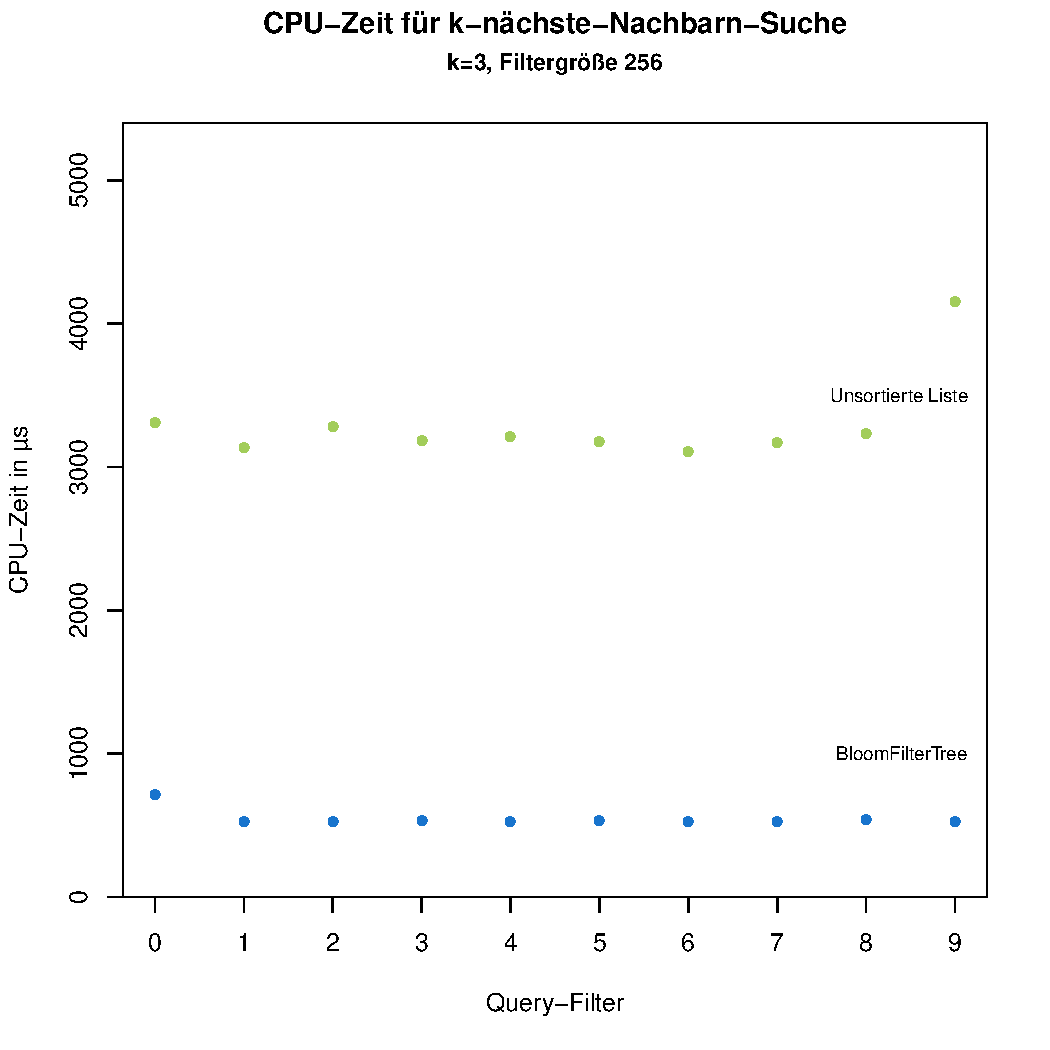
\includegraphics[scale=0.7]{pictures/cputime_nn3_256.pdf}\\
	\caption[CPU-Zeit für 3-nächste-Nachbarn-Suche mit 256 Bit-Bloom-Filtern]{CPU-Zeit für nächste-Nachbarn-Suche mit 256 Bit-Bloom-Filtern.}\label{fig:pic15}
	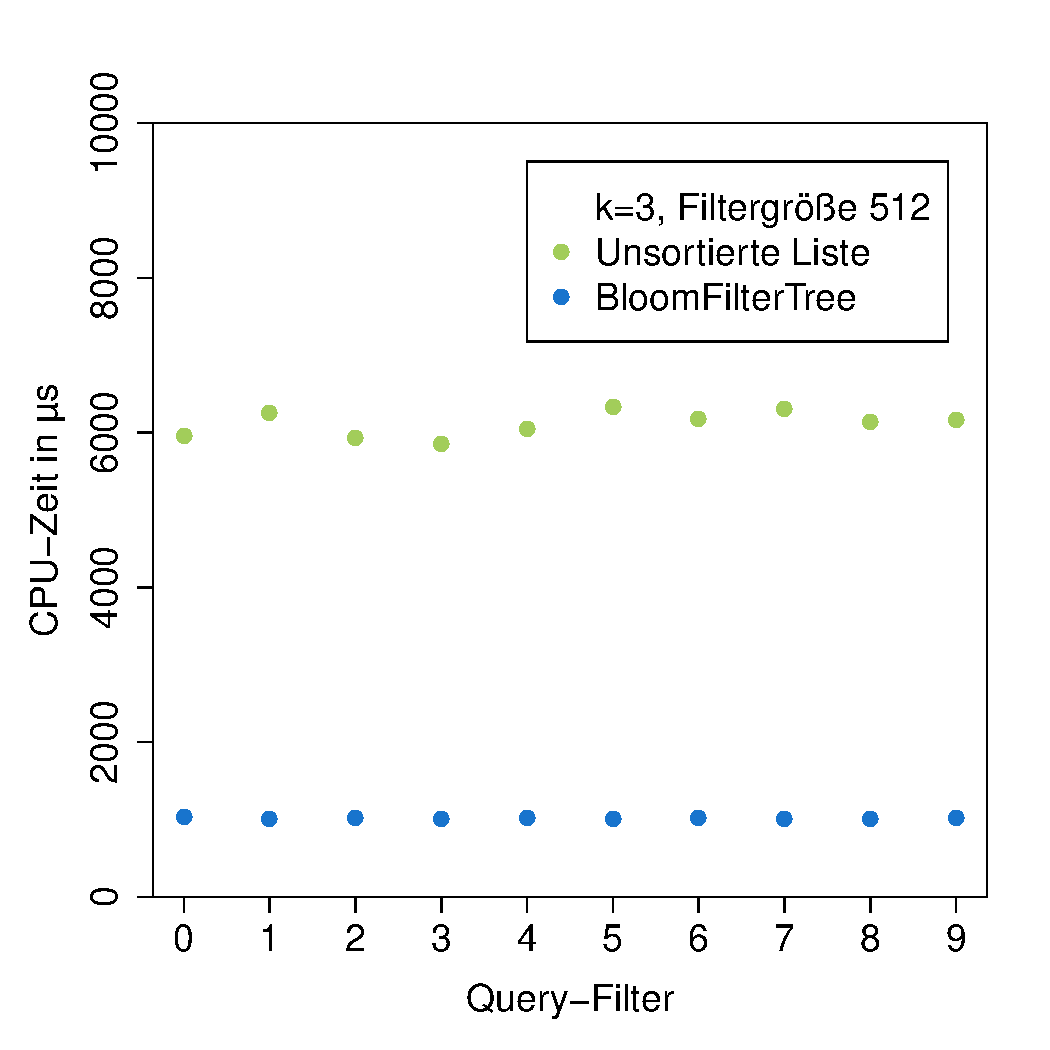
\includegraphics[scale=0.7]{pictures/cputime_nn3_512.pdf}\\
	\caption[CPU-Zeit für 3-nächste-Nachbarn-Suche mit 512 Bit-Bloom-Filtern]{CPU-Zeit für nächste-Nachbarn-Suche mit 512 Bit-Bloom-Filtern.}\label{fig:pic16}
\end{figure}
\paragraph*{Speicherbedarf}
Abbildung \ref{fig:pic17} stellt den Speicherbedarf der angelegten Objekte dar. Der Speicherbedarf für Objekte vom Typ BloomFilterTree ist darin blau markiert. Der Speicherbedarf für Objekte vom Typ \texttt{std::vector<BloomFilter>} ist grün markiert. 
\begin{figure}[hptb]
	\centering
	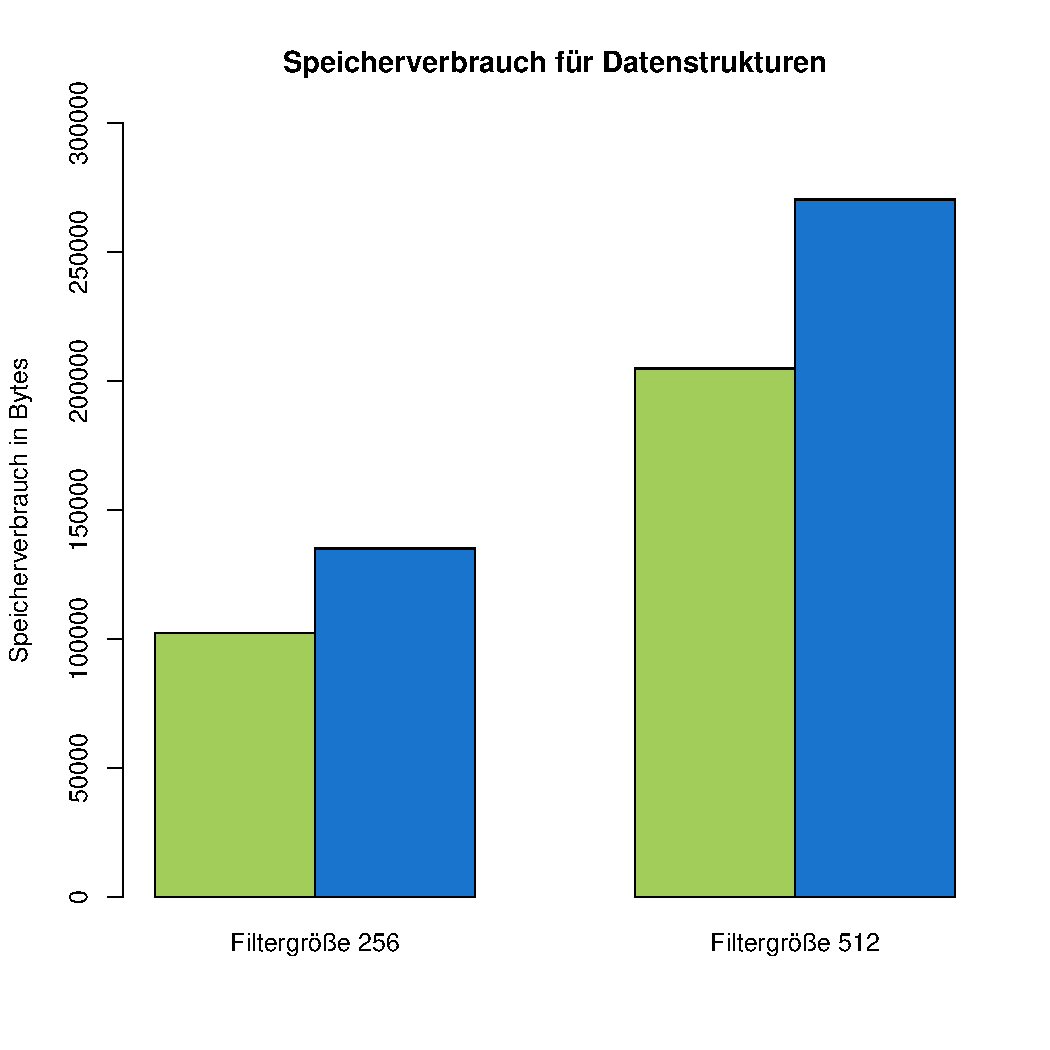
\includegraphics[scale=0.7]{pictures/mem.pdf}\\
	\caption[Speicherbedarf für BloomFilterTree und unsortierte Liste]{Speicherbedarf für BloomFilterTree und unsortierte Liste.}\label{fig:pic17} 
\end{figure}	
\paragraph*{Komplexität}
Abbildung \ref{fig:pic18} stellt die Komplexität der k-nächste-Nachbarn-Suche wie in Abschnitt \ref{sec:versuchsaufbau} beschrieben als Anzahl der zur Anfragebearbeitung nötigen Vergleiche dar. Die Ergebnisse für den BloomFilterTree sind darin blau, die Ergebnisse für die unsortierte Liste grün markiert.
\begin{figure}[hptb]
	\centering
	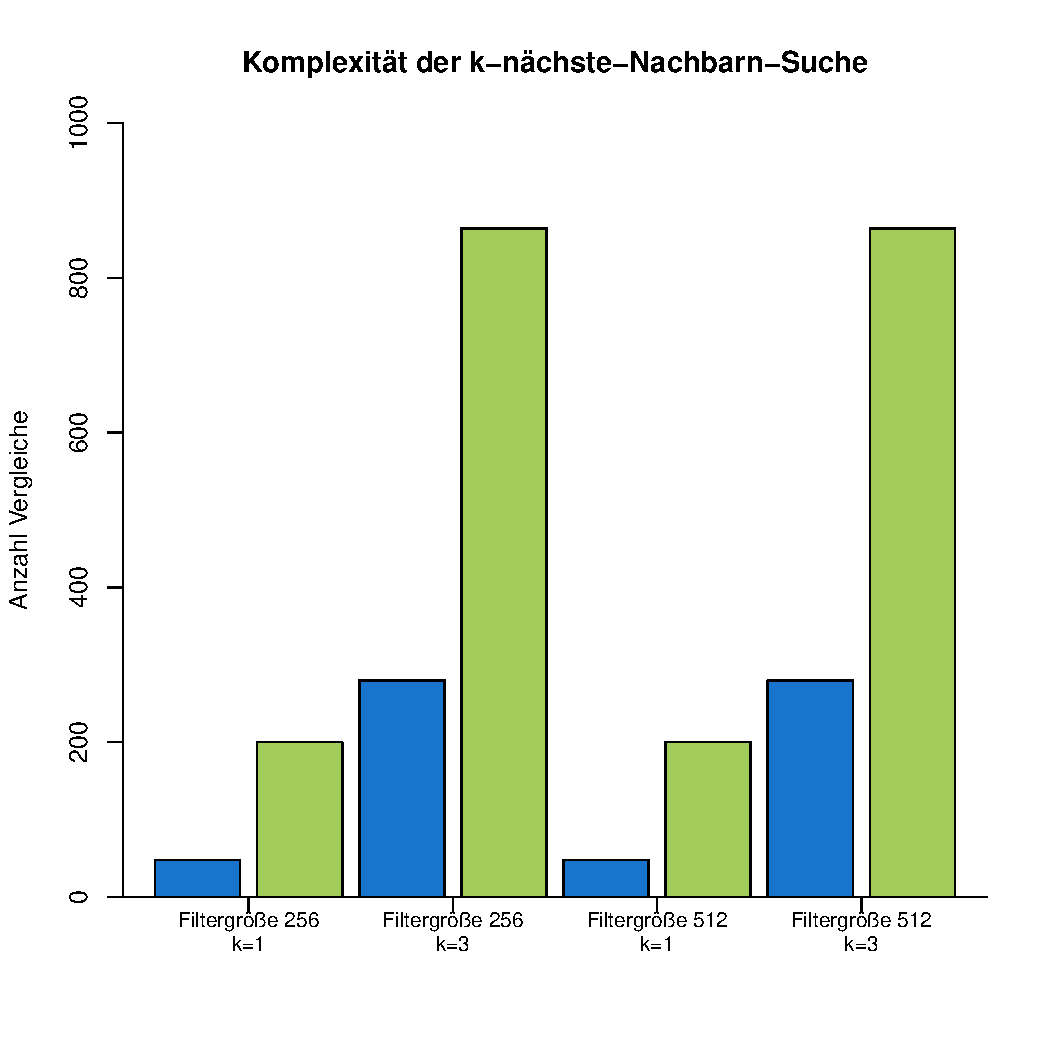
\includegraphics[scale=0.7]{pictures/compl.pdf}\\
	\caption[Anzahl zur \textit{k}-nächste-Nachbarn-Suche benötigter Vergleiche]{Anzahl zur \textit{k}-nächste-Nachbarn-Suche benötigter Vergleiche.}\label{fig:pic18}
\end{figure} 
\paragraph*{Aufbaukosten}
Abbildung \ref{fig:pic19} stellt die Aufbaukosten der angelegten Objekte dar. Die Aufbaukosten für Objekte vom Typ BloomFilterTree sind darin blau markiert. Die Aufbaukosten für Objekte vom Typ \texttt{std::vector<BloomFilter>} sind grün markiert. 
\begin{figure}[hptb]
	\centering
	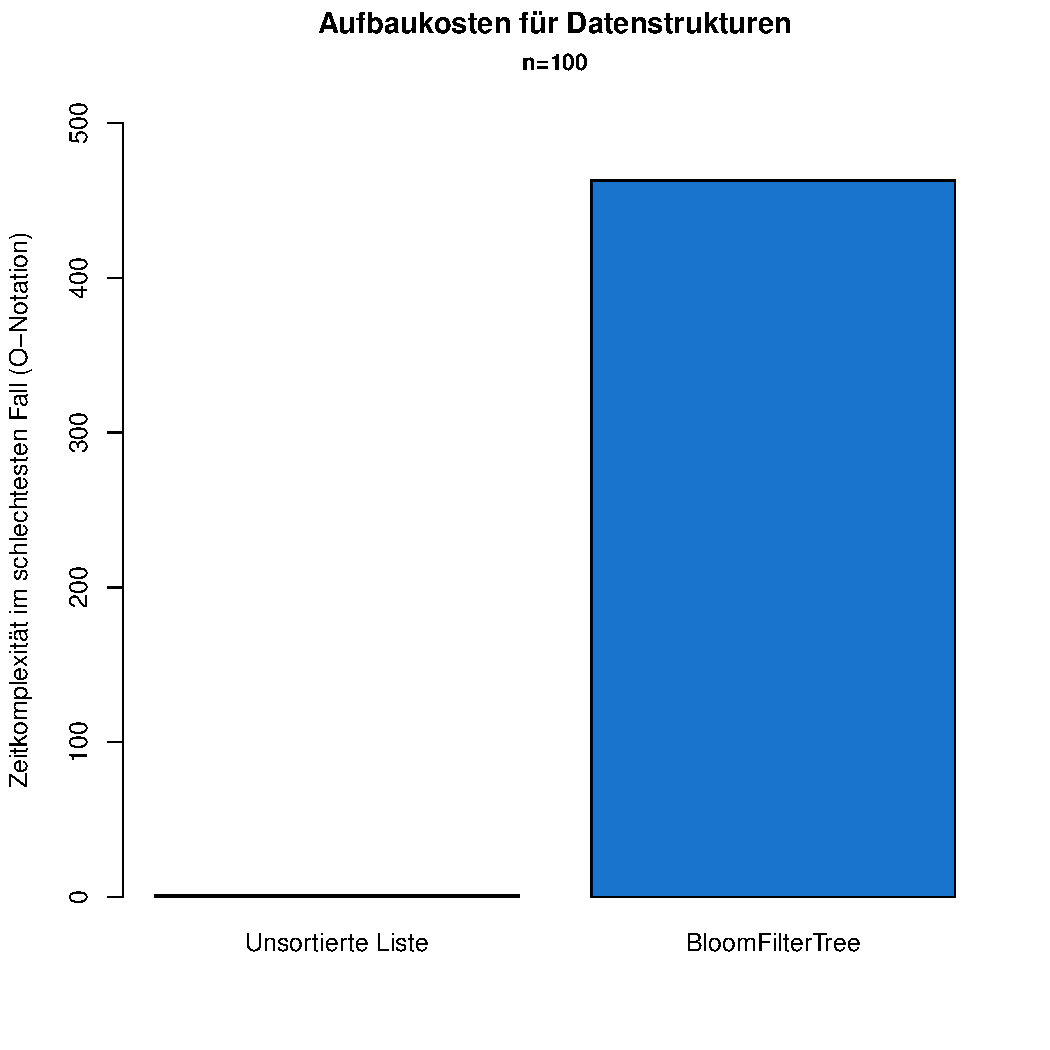
\includegraphics[scale=0.7]{pictures/cost.pdf}\\
	\caption[Aufbaukosten für BloomFilterTree und unsortierte Liste]{Aufbaukosten für BloomFilterTree und unsortierte Liste.}\label{fig:pic19}
\end{figure}
\newpage
\section{Interpretation}\label{sec:interpretation}
Wie in Abschnitt \ref{sec:datensatz} dargestellt, wurde die Evaluation mit zehn Anfragefiltern pro Experiment durchgeführt. Die soeben präsentierten Ergebnisse sind also dazu geeignet, den Mittelwert über einem Anfragevektor zu bilden und etwaige Ausreißer zu erkennen. Das gilt insbesondere für die Ergebnisse der CPU-Zeitmessung, die in der Regel wegen schwankender Nutzlast der verwendeten Maschine und nicht exakt vorhersehbaren CPU-Schedulings gewissen Schwankungen unterliegen. Demnach kann hierfür das Minimum der erzielten Werte als Benchmark für die \textit{k}-nächste-Nachbarn-Suche angesehen werden. 
\paragraph*{Ergebnisqualität}
Die Ergebnisse der \textit{k}-nächste-Nachbarn-Suche stimmen zum größten Teil mit den Sollwerten überein. Bei der nächsten-Nachbarn-Suche mit 256 Bit-Bloom-Filtern treten zwei abweichende Ergebnisse auf (vgl. Abbildung \ref{fig:pic7}). Bei der 3-nächste-Nachbarn-Suche mit 256-Bit-Filtern treten bei 30 Ergebnissen fünf abweichende Einzelergebnisse auf. Bei der 3-nächste-Nachbarn-Suche mit 512-Bit-Filtern treten bei 30 Ergebnissen sechs abweichende Einzelergebnisse auf. 

Der quadratische Fehler für diese Fälle beträgt bei der nächste-Nachbarn-Suche mit 256 Bit-Bloom-Filtern maximal 0.0008548022, andernfalls 0. Bei der 3-nächste-Nachbarn-Suche mit 256 Bit-Bloom-Filtern beträgt der mittlere quadratische Fehler bei abweichenden Messwerten maximal 0.0002956207, andernfalls 0. Bei der 3-nächste-Nachbarn-Suche mit 512 Bit-Bloom-Filtern beträgt er maximal 0.00008640455, andernfalls 0.

Das bedeutet: Nächste-Nachbarn-Anfragen werden mit dem entwickelten Verfahren in den meisten Fällen korrekt beantwortet. Mit einigen wenigen Fällen werden suboptimale Antworten zurückgegeben. Diese sind dennoch als "`gute"' Antworten bezüglich des verwendeten Distanzmaßes und des maximalen quadratischen Fehlers zu bezeichnen. Dieses Resultat ist essentiell für die Bewertung des entwickelten Verfahrens. Es kann nur dann zuverlässig eingesetzt werden, wenn es in einem Großteil der Fälle zufriedenstellende Ergebnisse bzw. optimale Antworten liefert. 
\paragraph*{CPU-Zeit}
Die drastisch reduzierte CPU-Zeit ist als entscheidender Vorteil des entwickelten Verfahrens zu betrachten. In der verwendeten Versuchsanordnung kommt sie vor allem bei der 3-nächste-Nachbarn-Suche zum Tragen. Abbildung \ref{fig:multipic1} stellt die jeweils erreichte CPU-Zeitersparnis gegenüber:
\begin{figure}[hpbt]
 \centering
  %%----start of first subfigure----
  \subfloat[CPU-Zeitersparnis für nächste-Nachbarn-Suche mit 256-Bit-Bloom-Filtern]{
   \label{fig:multipic1:a} %% label for first subfigure
   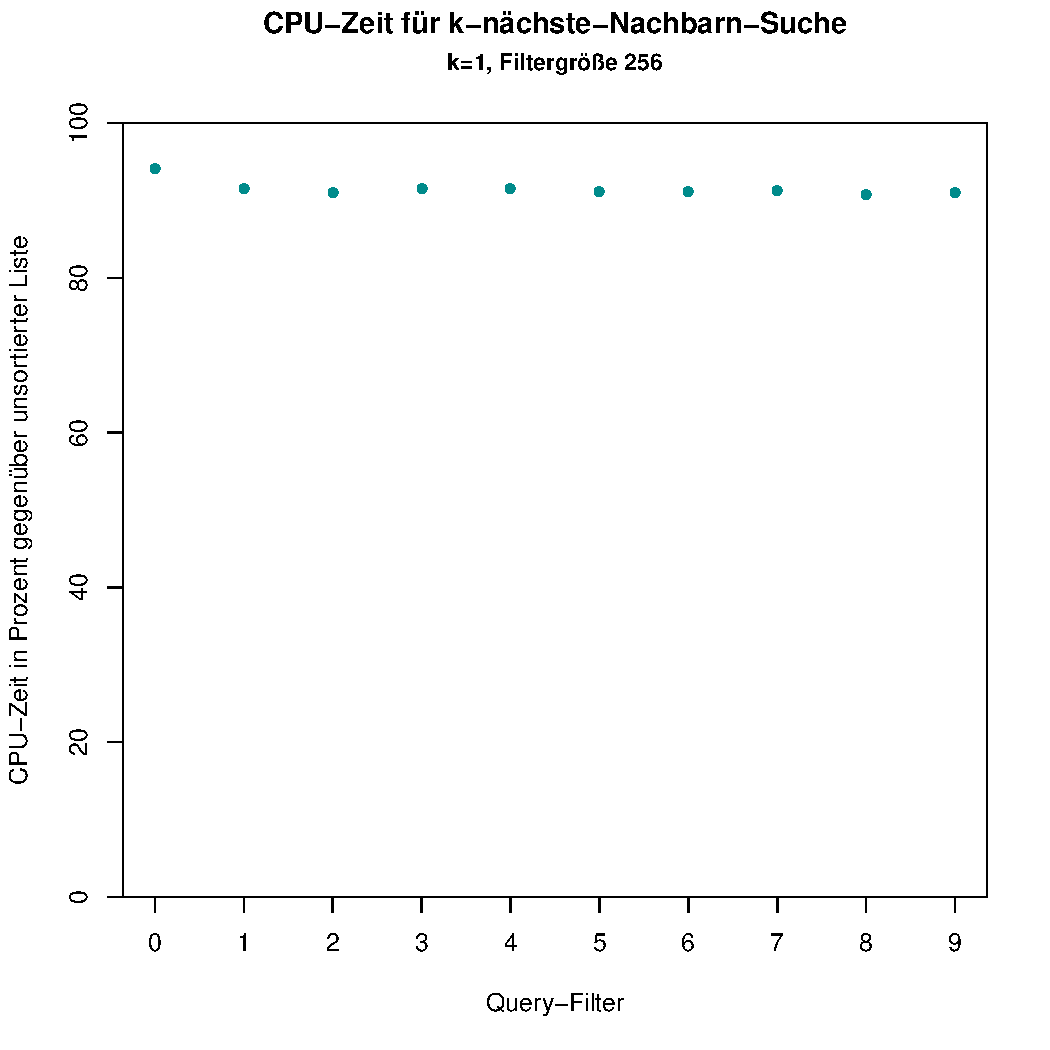
\includegraphics[width=0.48\linewidth]{pictures/percent_time_nn_256.pdf}}
  \hspace{0.01\textwidth}
  %%----start of second subfigure----
  \subfloat[CPU-Zeitersparnis für nächste-Nachbarn-Suche mit 512-Bit-Bloom-Filtern]{
   \label{fig:multipic1:b} %% label for second subfigure
   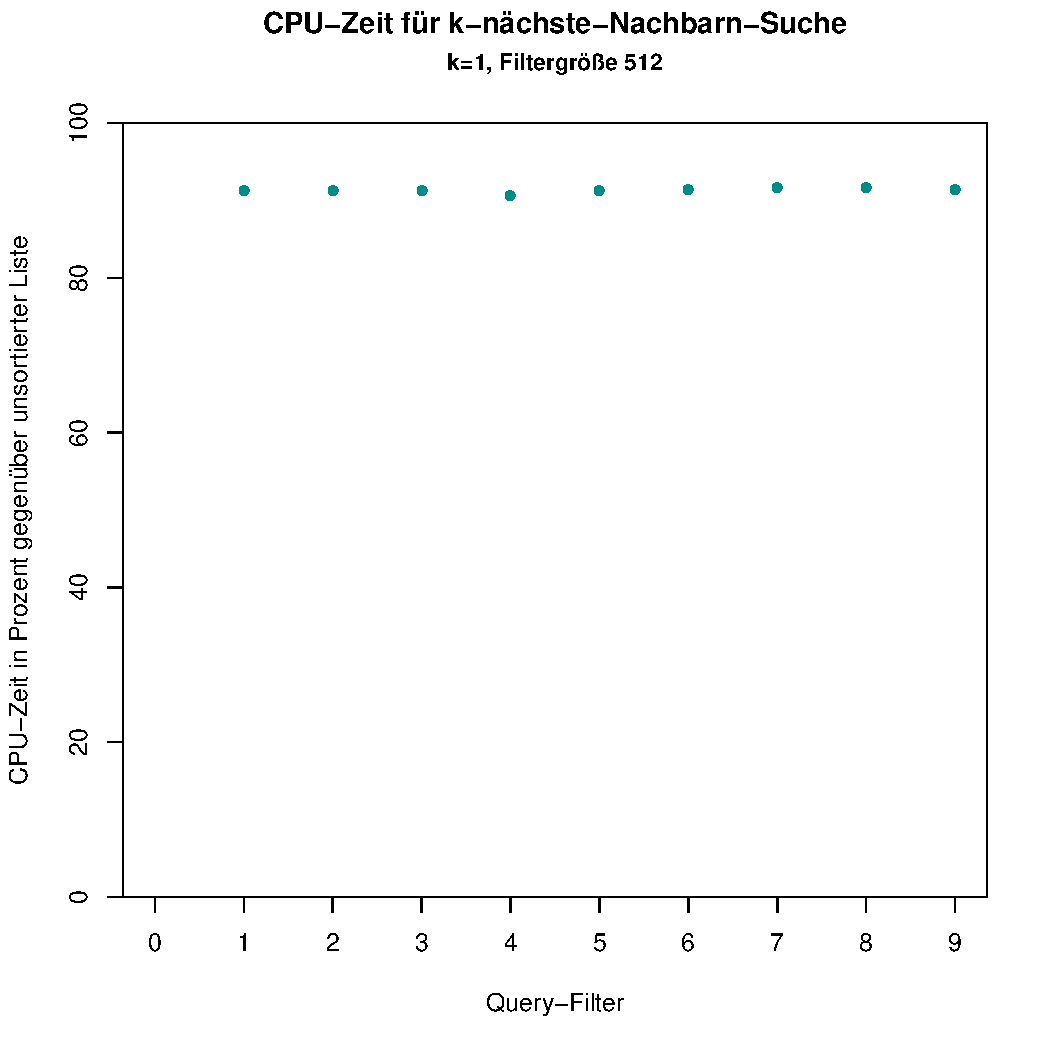
\includegraphics[width=0.48\linewidth]{percent_time_nn_512.pdf}}\\[0pt] % horizontal break
  %%----start of third subfigure----
  \subfloat[CPU-Zeitersparnis für 3-nächste-Nachbarn-Suche mit 256-Bit-Bloom-Filtern]{
   \label{fig:multipic1:c} %% label for third subfigure
   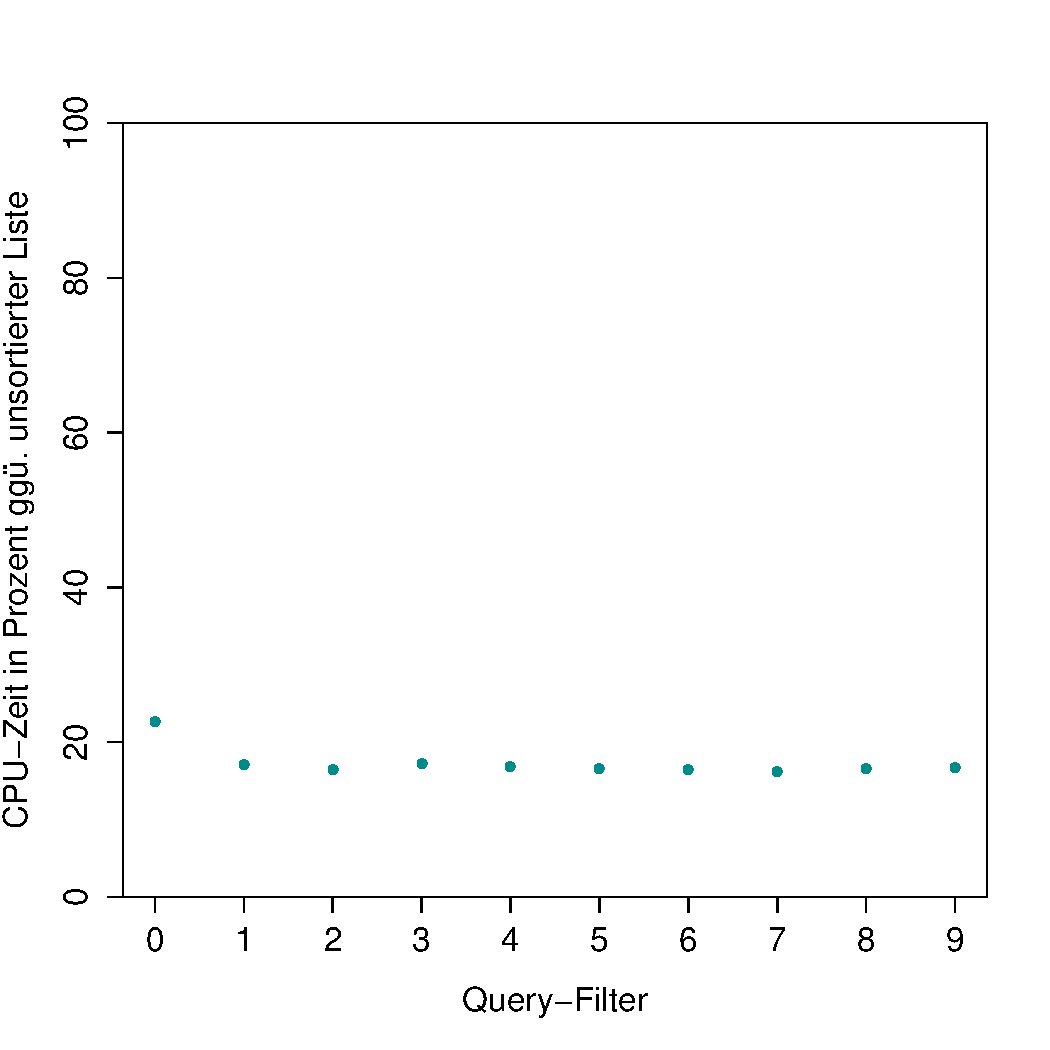
\includegraphics[width=0.48\linewidth]{pictures/percent_time_nn3_256.pdf}}
  \hspace{0.01\textwidth}
  %%----start of fourth subfigure----
  \subfloat[CPU-Zeitersparnis für 3-nächste-Nachbarn-Suche mit 512-Bit-Bloom-Filtern]{
   \label{fig:multipic1:d} %% label for fourth subfigure
   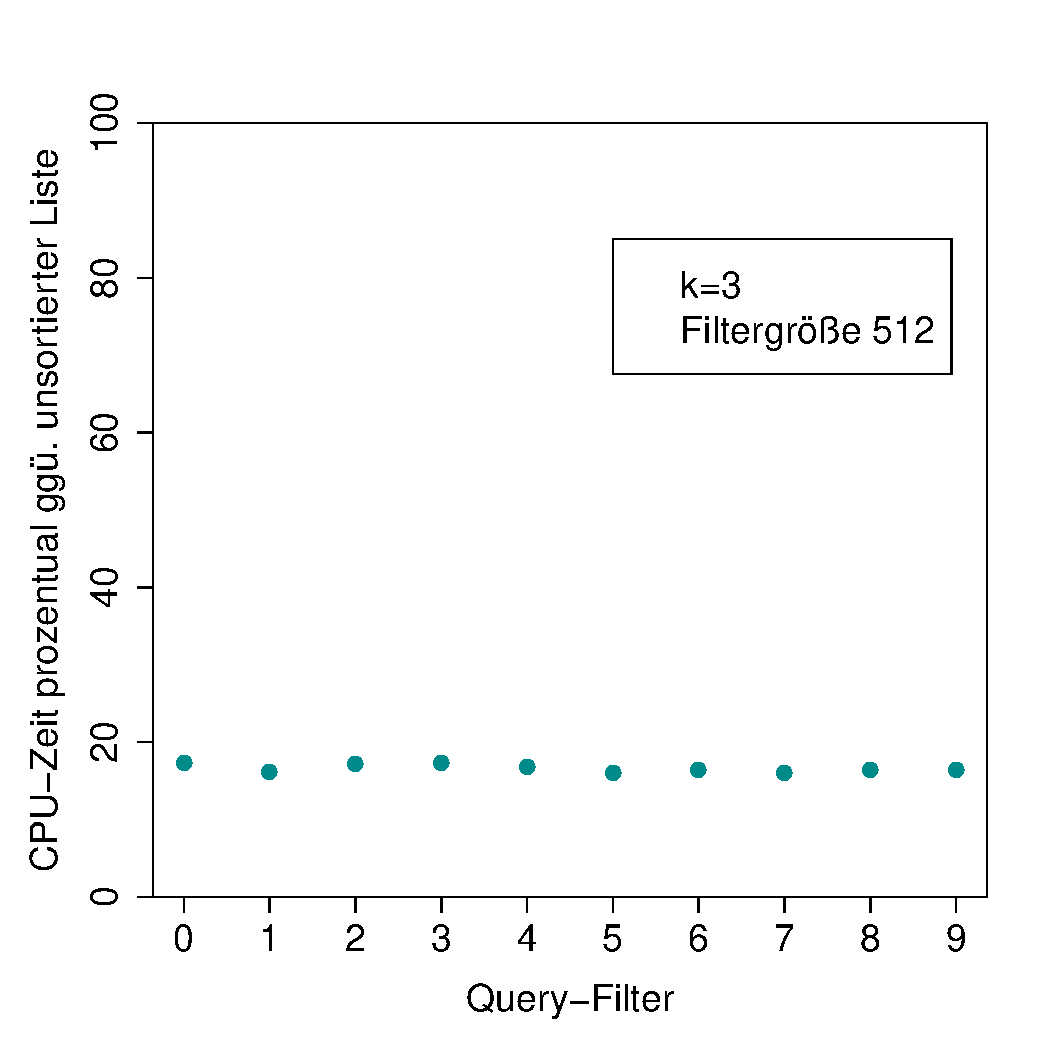
\includegraphics[width=0.48\linewidth]{pictures/percent_time_nn3_512.pdf}}
 \caption[CPU-Zeitersparnis für k-nächste-Nachbarn-Suche im BloomFilterTree]{CPU-Zeitersparnis für k-nächste-Nachbarn-Suche im BloomFilterTree.}
 \label{fig:multipic1} %% label for entire figure
\end{figure}
Daran wird deutlich: Die Zeitersparnis wächst mit dem Parameter \textit{k} und der Filtergröße, doch auch bei $k=1$ wird bereits CPU-Zeit eingespart. Es ist zu erwarten, dass bei größeren BloomFilterTree-Objekten, höheren Anzahlen an Filtern und ggf. größeren Filtern die Zeitersparnis noch deutlich gesteigert werden kann: 

Beim hier verwendeten Versuchsaufbau werden i.d.R Bäume mit drei Ebenen aufgebaut, d.h. bei einer Punktanfrage wird auch bei bestehenden Teil- und Obermengenbeziehungen ein großer Teilbaum durchsucht bzw. ein großer Bereich der Blattebene traversiert. Bei größerer Höhe des Baums durch mehr eingefügte Filter kommen damit die Vorteile des entwickelten Verfahrens deutlicher zum Tragen. Wie in Abbildung \ref{fig:multipic1} erkennbar, gilt ebenso für höhrere Filtergrößen. Die CPU-Zeitersparnis zeigt sich bei Anfragen mit $k>1$ besonders deutlich. Auch hier ist zu erwarten, dass sich die Vorteile des entwickelten Verfahrens bei höheren Bäumen und Filteranzahlen sowie größeren Filtern noch deutlich stärker zeigen.

Wie in Abschnitt \ref{sec:b+bäume} dargestellt, ist die Komplexität der Suchoperation im B$^+$-Baum abhängig vom Parameter \textit{t} ab, d.h. dem Grad des Baumes. Die hier verwendeten BloomFilterTree-Objekte haben Grad 3, d.h. der maximale Fan-out beträgt 7. Dieser Parameter kann beim Anlegen eines BloomFilterTree-Objekts in der eigenen Implementierung frei gewählt werden. In der Praxis werden deutlich höhere Verzweigungsgrade verwendet, z.B. mit 10.000 Elemente pro innerem Knoten beim Einsatz in Datenbank-Management-Systemen. Es ist daher anzunehmen, dass die Anwendung für ein Szenario mit deutlich höheren Parameterwerten gut geeignet wäre. 
\paragraph*{Speicherbedarf}
Der zusätzliche Speicherbedarf beim BloomFilterTree gegenüber einem Bloom-Filter-Vektor ergibt sich durch die Allokierung eines Vereinigungsfilters für jeden Knoten. Er ist somit abhängig von der Anzahl der Knoten im Baum. Mit dem verwendeten Versuchsaufbau liegt er um 32\% für den BloomFilter gegenüber einem Bloom-Filter-Vektor. Auch hier ließe sich durch eine geringere Knotenanzahl, d.h. BloomFilterTree-Objekte mit höherem Verzweigungsgrad, noch Speicherplatz einsparen. 
\paragraph*{Komplexität}
Auch bezüglich der Zeitkomplexität, d.h. der Abschätzung der notwendigen Berechnungsschritte unabhängig von der gewählten Plattform, zeigt das entwickelte Verfahren erfreuliche Ergebnisse. Die Anzahl der nötigen Vergleiche bei der \textit{k}-nächste-Nachbarn-Suche beträgt 24\% bzw. 32\% beim BloomFilterTree gegenüber der unsortierten Liste. Auch hier ist zu erwarten, dass sich die Ergebnisse bei höheren Bäumen noch verbessern lassen, da bei der \textit{k}-nächste-Nachbarn-Suche nur der beste Pfad verfolgt wird. Bei höheren Bäumen werden somit mehr bzw. größere Teilbäume abgeschnitten und müssen nicht betrachtet werden. 
\paragraph*{Aufbaukosten}
Die Kosten für den Aufbau der Indexstruktur sind erwartungsgemäß ein Wermutstropfen. Auch wenn in der Praxis niedrigere Werte zu erwarten sind, da weniger als \textit{n} freie und "`gute"' IDs sortiert werden müssen, liegen die Aufbaukosten in $O(n\ast log(n))$. Das ist offensichtlich ein starker Zuwachs gegenüber einer unsortierten Liste, die sich z.B. durch ein Objekt vom Typ \texttt{std::vector} realisieren lässt. Andererseits kann davon ausgegangen werden, dass die Aufbaukosten in AMBIENCE deutlich seltener anfallen als z.B. in einem Verteilten System mit häufigem Ausscheiden und Hinzukommen von Knoten wie in den Abschnitten \ref{sec:bloom-netzwerk} und \ref{sec:bloom-index} beschrieben.
    \chapter{Zusammenfassung und Ausblick}\label{ch:zusammenfassung}
%Fassen Sie Ihre gesamte Arbeit noch einmal kurz zusammen. Ziehen Sie ein Fazit und geben Sie gegebenenfalls einen Ausblick darüber, wie Ihrer Meinung nach noch offen stehende Probleme angegangen werden könnten.

Zukünftige Arbeiten: 
* Löschen aus BloomFilterTree
* All-Pairs-Similarity-Search nach Bayardo et al. 
* Restrukturierungskosten 
* Andere/realistischere B+Bäume
%
% =================================================================================================
% place your appendix here
% -------------------------------------------------------------------------------------------------
%
    \appendix
    % % -------------------------------------------------------------------------------------------------
%      MDSG Latex Framework
%      ============================================================================================
%      File:                  appendix.tex
%      Author(s):             Michael Duerr
%      Version:               1
%      Creation Date:         30. Mai 2010
%      Creation Date:         30. Mai 2010
%
%      Notes:                 - Place your appendix here
%                             - Use the same commands (`chapter', `section', ...) as in main text
% -------------------------------------------------------------------------------------------------
%
\chapter{Anhang}\label{ch:anhang}
\section{Die Klasse \texttt{BloomFilterTree}}\label{sec:BloomFilterTree.hpp}
\small{
\begin{verbatim}
//  BloomFilterTree.hpp, Judith Greif
//  Description: Header for class BloomFilterTree

#ifndef BloomFilterTree_hpp
#define BloomFilterTree_hpp

#include "BloomFilterNode.hpp"
#include "BloomFilterIndexNode.hpp"
#include "BloomFilterLeaf.hpp"

using namespace std;

class BloomFilterTree {
    
private:
    int t;                          // Order = minimum degree
    int filtersize;                 // Size of associated Bloom filters (# of bits)
    
public:
    BloomFilterNode *root;          // Pointer to root node   
    BloomFilterTree(int _t, int _s);
    ~BloomFilterTree();   
    BloomFilterNode *getRoot();
    
    // Tree management
    void traverse();
    void traverseFilters();
    double computeMinJaccard(BloomFilter *filter);
    double computeMaxJaccard(BloomFilter *filter);
    int getMinJaccardKey(BloomFilter *filter);
    BloomFilter *getMinJaccardFilter(BloomFilter *filter);
    int getMinKey();
    int getMaxKey();
    vector<BloomFilter> collectAllFilters();
    int countFilters();
    int countUnionFilters(); 
    int computeSubsetId(BloomFilter *filter);
    int computeSupersetId(BloomFilter *filter);
    bool contains(int k);
    BloomFilterNode *search(int k);
    vector<pair<int, double>>computeAllDistances(BloomFilter *filter);
    vector<pair<int, double>>computekDistances(BloomFilter *filter, int k);
    int countLeaves(); 
    
    // Measurement and comparison
    vector<pair<BloomFilter, double>> compare(BloomFilter *filter, int k);
    vector<int> compareMem();
    vector<double> compareConstrCost();
    vector<int> compareComplSimQuery(BloomFilter *filter);
    vector<int> compareComplSimQueryVec(BloomFilter *filter, int k);
    
    // Insertion
    void insert(BloomFilter *filter);
    void insertAsSets(BloomFilter *filter);
    
    // Similarity queries
    BloomFilter *simQuery(BloomFilter *filter);
    vector<BloomFilter*> simQueryVec(BloomFilter *filter, int k);
};

#endif
\end{verbatim}
}
\newpage
\section{Die Klasse \texttt{BloomFilter}}\label{sec:BloomFilter.hpp}
\small{
\begin{verbatim}
//  BloomFilter.hpp, Judith Greif
//  Description: Header for class BloomFilter

#ifndef BloomFilter_hpp
#define BloomFilter_hpp

#include <iostream>
#include <vector>
#include <cstdlib>
#include <random>
#include <math.h>
#include <string>
#include <functional>

using namespace std;

const int NUM_FILTERS = 100;
const int NUM_ELEMENTS = 50;
const int NUM_QUERYFILTERS = 10;
const int seed = rand();

class BloomFilter {
    
private:
    int id;
    int count;                  // # of elements inserted
    int size;                   // # of bits
    int d;                      // # of hash functions
    int *data;
    
public:
    BloomFilter();
    BloomFilter(const BloomFilter& fSource);
    BloomFilter(int _id, int _size);
    ~BloomFilter();   
    BloomFilter & operator = (const BloomFilter &fSource);   
    void setId(int value);
    int getId();
    int getSize();
    void setValue(int index, int value);
    int *getData();   
    void printData();
    void printArr();
    void initRandom();
    double fractionOfZeros();
    double eSize();
    BloomFilter *logicalOr(BloomFilter *filter);
    BloomFilter *logicalAnd(BloomFilter *filter);
    bool isSubset(BloomFilter *filter);
    bool isSuperset(BloomFilter *filter);
    int mySupersetCount();
    int mySubsetCount();
    int binomialCoefficient(int n, int k);
    int setOnes();
    int setZeros();
    int validOnes();
    int possibleFreeZeros();
    int possibleAddedOnes();
    double setUnion(BloomFilter *filter) const;
    double setIntersection(BloomFilter *filter) const;
    double computeAmbienceJaccard(BloomFilter *filter);
    double computeJaccard(BloomFilter *filter) const;
    double eUnion(BloomFilter *filter);
    double eIntersect(BloomFilter *filter);
    void add(string &elem);
    void increment();
    int getNumHashes();
    bool checkCorrectFillDegree();
};

#endif
\end{verbatim}
\newpage
\section{Die Methode \texttt{computeSubsetId()} der Klasse \texttt{BloomFilterLeaf()}}\label{sec:computeSubsetId()}
\small{
\begin{verbatim}
int BloomFilterLeaf::computeSubsetId(BloomFilter *filter) {
    vector<pair<int, double>> subsets;
    vector<int> freeIds;
    vector<pair<int, int>> goodIds;
    BloomFilterLeaf *tmp = this;
    double jacc;
    int minId = filters[0]->getId()-1;
    int maxId;
    int optId;
    bool no_subsets = true;
    while (tmp != NULL) {
        
        // Collect all filters that filter is subset of
        for (int i=0; i<tmp->getCount(); i++) {
            if ((tmp->filters[i])->isSubset(filter)) {
                jacc = computeJaccard(tmp->filters[i], filter);
                subsets.push_back(make_pair(tmp->filters[i]->getId(), jacc));
                no_subsets = false;
            }
        }
        maxId = tmp->filters[tmp->getCount()-1]->getId()+1;
        tmp = tmp->getNext();
    }
    
    // Sort subsets by jacc distances in ascending order
    sort(subsets.begin(), subsets.end(), [](const pair<int, double> &left, 
    const pair<int, double> &right) {
        return left.second < right.second;
    });
    
    // Collect free ids
    tmp = this;
    freeIds.push_back(minId);
    freeIds.push_back(maxId);
    while (tmp != NULL) {
        for (int i=0; i<tmp->getCount()-2; i++) {
            for (int j=tmp->filters[i]->getId()+1; j<tmp->filters[i+1]->getId(); j++) {
                if (j<tmp->filters[i+1]->getId()) {
                    freeIds.push_back(j);
                }
            }
            if (tmp->getCount() < tmp->getMax()) {
                if (tmp->getNext() != NULL) {
                    int start = tmp->filters[tmp->getCount()-1]->getId()+1;
                    int last = tmp->getNext()->filters[0]->getId();
                    for (int j=start; j<last; j++) {
                        freeIds.push_back(j);
                    }
                }
            }
            
        }
        tmp = tmp->getNext();
    }
    sort(freeIds.begin(), freeIds.end(), less<int>());
    
    // If there are no subsets, return smallest free id as pair with numerical distance 0
    if (no_subsets == false) {
        
        // Determine optimal id
        // Check subsets in ascending order
        // Get next greater and smaller id
        int distNeg = subsets[0].first - minId;
        int distPos = maxId - subsets[0].first;
        for (int i=0; i<subsets.size(); i++) {
            optId = subsets[i].first;
            int j=0;
            while (freeIds[j] < subsets[i].first) {
                if (optId-freeIds[j] < optId-minId) {
                    minId = freeIds[j];
                    distNeg = optId-minId;
                }
                j++;
            }
            
            j=freeIds.size()-1;
            while (freeIds[j] > subsets[i].first) {
                if (freeIds[j]-optId < maxId-optId) {
                    maxId = freeIds[j];
                    distPos = maxId-optId;
                }
                j--;
            }
            goodIds.push_back(make_pair(minId, distNeg));
            goodIds.push_back(make_pair(maxId, distPos));
        }
        
        // Sort next smaller and greater ids by numerical distance in ascending order
        sort(goodIds.begin(), goodIds.end(), [](const pair<int, int> &left, 
        const pair<int, int> &right) {
            return left.second < right.second;
        });
    }
    else {
        goodIds.push_back(make_pair(freeIds[0], 0));
    }
    
    // Return first element
    return goodIds[0].first;
}
\end{verbatim}
}
    % further appendix
%
% =================================================================================================
% comment \listoffigures and/or \listoftables if not wanted
% -------------------------------------------------------------------------------------------------
%
    \backmatter
    \listoffigures                                % list of figures (uncomment if wanted)
    % \listoftables                                 % list of tables (uncomment if wanted)
    % \lstlistoflistings                            % list of listings (uncomment if wanted)
%
% =================================================================================================
% place your bibliography here
% -------------------------------------------------------------------------------------------------
%
    \begin{spacing}{0.9}                          % save some space
    	   %\nocite{*}
       \bibliographystyle{geralpha}               % for german thesis
       %\bibliographystyle{alpha}                 % for english thesis
       \bibliography{bibliography}                % the location of bib file
    \end{spacing}
\end{document}
%
% =================================================================================================
% end of document
% -------------------------------------------------------------------------------------------------
%
